\chapter{Monte Carlo Radiative Transfer and Ionization}

\epigraph{``I'm splashing greys where once was glowing white''}{{\sl Mike Vennart, Silent/Transparent}}

In the previous chapters I have given an introduction to the field and 
some relevant background relating to accretion 
discs and their associated outflows. Now it proves useful
to discuss the specific {\em methods} I will use
in order to answer some of the questions raised so far.
In particular, I will discuss radiative transfer and photoionization
techniques.

{\sl Notation: This section contains a lot of algebraic quantities and sums over
ions, levels, and so on. Throughout, I use $N$ to denote fractional
populations of ions and $n$ to denote fractional populations of levels. 
The primed quantities $\ellp$ and $\up$ follow the convention of 
\cite{lucy2002} in that they denote sums over all lower/upper levels.
The symbol ${\cal R}$ denotes a total rate (radiative + collisional), 
and the symbol $C$ is a collisional rate, whereas ${\cal C}$ is a cooling 
rate. Starred quantities are evaluated at the stated temperature but 
in local thermodynamic equilibrium, following \cite{mihalas}. An $S$ 
superscript denotes that the estimator pertains to simple-atoms.
}



\section{Fundamentals of Radiative Transfer}

\begin{figure}
\centering
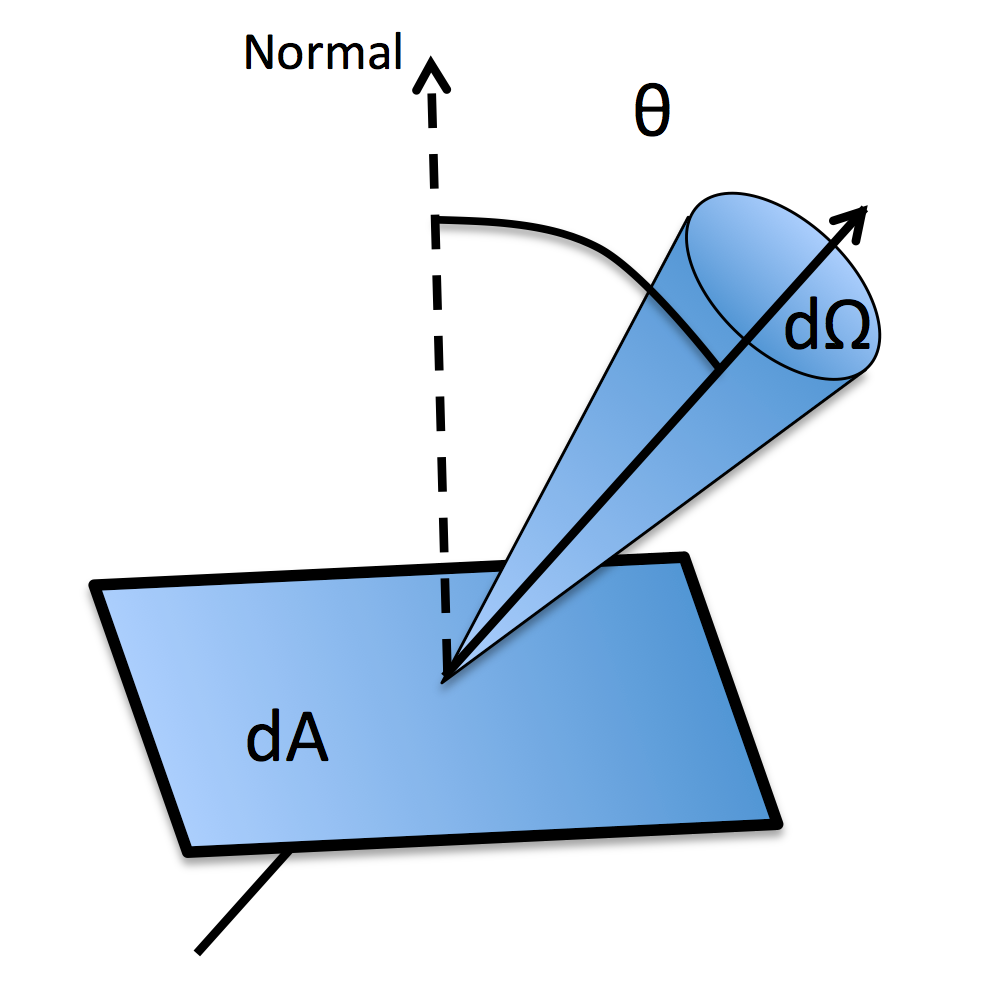
\includegraphics[width=0.5\textwidth]{figures/03-radtrans/rays_schematic.png}
\caption
{
A schematic showing a ray obliquely incident on a surface of area $dA$.
The labeled quantities are used in the definition of specific intensity.
} 
\label{fig:ray}
\end{figure}

Let us consider a ray passing through a reference surface $dA$ and 
making an angle $\theta$ with the normal to this surface. The energy
flow can then be related to the
{\em specific intensity}, $I_\nu$, by
\begin{equation}
I_\nu = \frac{dE}{d\Omega~dt~dA~d\nu},
\end{equation}
which has units of ${\rm erg~s^{-1}~Hz^{-1}~sr^{-1}~cm^{-2}}$. The specific
intensity is the most fundamental quantity of radiative transfer as it describes 
everything about the radiation field; its time, angular, spatial and frequency
dependence.
By successively multiplying by $\cos \theta$ and integrating over solid angle we 
can obtain the first and second `moments' of the radiation field. These
are the flux, $F_\nu$ and momentum flux, $p_\nu$, respectively, given by
\begin{equation}
F_\nu = \int I_\nu \cos \theta~d \Omega,
\end{equation}
\begin{equation}
p_\nu = \frac{1}{c} \int I_\nu \cos^2 \theta~d \Omega.
\end{equation}
The {\em mean intensity}, $J_\nu$, is
\begin{equation}
J_\nu = \frac{1}{4 \pi} \int I_\nu~d \Omega.
\end{equation}
The mean intensity is particularly
useful when one wants to ignore the solid angle dependence of the radiation,
for example when considering the impact of an ionizing radiation field.

The equation describing the specific intensity change along a path element $ds$
is the radiative transfer equation, 
\begin{equation}
\frac{d I_\nu}{ds} = -\kappa_\nu I_\nu + j_\nu, 
\label{eq:rte}
\end{equation}
where $\kappa_\nu$ and $j_\nu$ are the absorption and emission coefficients respectively.
If we define the optical depth $d \tau_\nu = \kappa_\nu ds$ this can be recast as
\begin{equation}
\frac{d I_\nu}{d \tau_\nu} = -I_\nu + S_\nu
\label{eq:formal_rte}
\end{equation}
where $S_\nu=j_\nu/\kappa_\nu$ is the source function. This equation
can be solved to give the {\em formal solution to the radiative transfer equation}:
\begin{equation}
I_\nu = I_{\nu,0}~e^{-\tau_\nu} + \int^{\tau_\nu}_0 S_\nu (\tau^\prime_\nu)~e^{\tau^\prime_\nu-\tau_\nu} d \tau^\prime_\nu.
\label{eq:rte_solution}
\end{equation}
A useful limit is when the source function is constant in the absorbing medium, in which case
the integral can be easily evaluated to give
\begin{equation}
I_\nu = I_{\nu,0}~e^{-\tau_\nu} + S_\nu (1 - e^{-\tau_\nu}).
\label{eq:rte_solution}
\end{equation}

% The mean intensity, $J_\nu$ is a particularly useful quantity when calculation the ionization
% state 



\subsection{Spectral Line Formation}

From the above equations, it is trivial to show how emission and absorption lines form when
the source function is approximately constant.
Say we have a plasma illuminated by a blackbody of temperature $T_0$, such that
$I_{\nu,0} = B_\nu (T_0)$. The plasma layer then has a different temperature, $T$,
such that $S_\nu = B_\nu (T)$ in that medium. By inspecting equation~\ref{eq:rte_solution}
we can see that if we are optically thick within the line, but optically
thin in the continuum, then inside the line the source term is dominant and outside 
the line the first $I_{\nu,0}~e^{-\tau_\nu}$ term dominates. Therefore, if $T > T_0$ we will 
see an emission line, and if $T < T_0$ we will see an absorption line. 
% This approach describes line emission in the blackbody limit; for more complicated SED shapes
% it is necessary to construct simple model atoms.

\subsection{Local Thermodynamic Equilibrium}
\label{sec:lte}


An important physical limit is that of local thermodynamic equilibrium (LTE).
This is a first-order way to describe the physical conditions of a plasma, and assumes
that all the properties of the plasma, such as the level populations and source function,
are the same as those in thermodynamic equilibrium for local values of 
temperature and density. For this to be the case, the principle of 
{\em detailed balance} must also apply, in which every 
process by which electrons transition in state must be exactly 
balanced by its inverse process. In LTE, the electron temperature, 
$T_e$, is equal to the temperature of the radiation, $T_R$, and
the source function is given by a blackbody, i.e. $S_\nu = B_\nu (T_R)$.
Three microscopic requirements of LTE also follow \citep{mihalas}:

a) The velocities of the electrons and ions in the plasma obey Maxwellian
distributions, such that
\begin{equation}
f(v) = 4 \pi \left( \frac{m_e}{2 \pi kT_e} \right)^{3/2} v^2 
\exp \left( - \frac{m_ev^2}{2kT_e} \right),
\label{eq:maxwellian}
\end{equation}
where $m_e$ is the mass of an electron.

\smallskip

b) The ionization state of the plasma is governed by the {\em Saha equation},
which states that two adjacent ions have relative populations given by
\begin{equation}
\frac{N_{i+1}n_e}{N_i} = \frac{2g_{i+1}}{g_i} 
\left( \frac{2 \pi m_e kT_e}{h^2} \right)^{3/2}
\exp(-h \nu_0/kT),
\label{eq:saha}
\end{equation}
where $g_i$ is the multiplicity of ion $i$ and $\nu_0$ is the threshold frequency.

\smallskip

c) The excitation state of the plasma is governed by {\em Boltzmann statistics}.
A level $j$ then has a population relative to ground governed by
\begin{equation}
\frac{n_{j}}{n_1} = \frac{g_j}{g_1} \exp(-E_j/kT_e), 
\label{eq:boltzmann}
\end{equation}
where $E_j$ is the energy difference between the two levels and 
$g_j$ is the statistical weight of level $j$. 

\smallskip

Although these three assumptions are sometimes valid, in many astrophysical situations
there can be large departures from LTE. A good example of these departures is when
the SED is not a blackbody and is affected by absorption -- 
as is the case in AGN and other accreting systems. The Maxwellian assumption 
is probably the most reliable, but even this may break down
when high-energy photons create suprathermal electron distributions 
\citep{humphrey2014}. 

\subsubsection{Dilute Approximation}
\label{sec:dilute}
A first step away from LTE is to introduce the dilute approximation. In this case,
I relax the assumption that $T_R = T_e$, and assume that the mean intensity is given
by a dilute blackbody, i.e. 
\begin{equation}
J_\nu = W B_\nu (T_R),
\label{eq:dilute_jnu}
\end{equation}
where $W$ is the dilution factor. The ionization state can then be approximated 
with a modified Saha equation \citep{AL85,ML93},
\begin{equation}
\frac{N_{i+1} n_e}{N_i} = W [\xi + W(1-\xi)]
\left(\frac{T_e}{T_R}\right)^{1/2}
\left(\frac{N_{i+1}n_e}{N_i}\right)^*_{T_R}, \label{eq:ml93}
\end{equation}
where $\xi$ is the fraction of recombinations that go directly to
the ground state.
The excitation state can also be approximated (fairly poorly) 
with a dilute Boltzmann equation \citep{AL85,lucy1999sne}
\begin{equation}
\frac{n_{j}}{n_{1}} = W \frac{g_j}{g_{1}} \exp(-E_j/kT_R).
\label{eq:dilute_boltzmann}
\end{equation}

\subsection{The Two Level Atom}

The two level atom formalism is well described by \cite{mihalas}.
Let us consider an atomic model consisting of two levels that are linked 
by radiative and collisional transitions. 
Whilst this model is clearly a simplification, it nonetheless allows
for a first step into non-LTE line transfer and proves useful for modelling
the resonance lines briefly touched on in chapter 2.

To construct our simple model a few assumptions are necessary. The first
is the assumption of {\em statistical equilibrium}. This is the principle 
that the total rate into a given atomic level/state is equal to the 
total rate out of said state. This is clearly true whenever the timescale
to establish this equilibrium is shorter than the timescale on which
the ambient conditions change. The second is the assumption of
{\em complete redistribution (CRD)}, which states that the emission
and absorption line profiles are identical for a given transition. 
% This 
% assumption is somewhat analogous to the Sobolev approximation 
% (see section~\ref{sec:sobolev}). 
These assumptions allow us to formulate rate equations and derive the 
Einstein relations.

\subsubsection{Einstein coefficients}

Within a two level atom, the statistical equilibrium 
rate equation between two levels can be written as
\begin{equation}
B_{lu} \bar{J}_{ul} n_l = B_{ul} \bar{J}_{ul} n_u + A_{ul} n_u,
\label{eq:rate_einstein}
\end{equation}
where $B_{ul}$, $B_{ul}$ and $A_{ul}$ are the {\em Einstein coefficients}
for absorption, stimulated emission and spontaneous emission, respectively.
The `mean intensity in the line', $\bar{J}_{ul}$, is given by
\begin{equation}
\bar{J}_{ul} = \int \phi(\nu) J_\nu d\nu,
\label{eq:jbar}
\end{equation}
where $\phi(\nu)$ is the line profile.
We can then rearrange equation~\ref{eq:rate_einstein} in terms of 
the mean intensity, giving
\begin{equation}
\bar{J}_{ul} = \frac{A_{ul} / B_{ul}}{(n_l/n_u)(B_{lu}/B_{ul}) - 1}.
\label{eq:jbar2}
\end{equation}
In LTE, $\bar{J}_{ul} = B_\nu (T)$ and the level populations obey Boltzmann statistics, 
so equations~\ref{eq:planck}, \ref{eq:boltzmann}
and \ref{eq:jbar2}  can be combined to give
\begin{equation}
\frac{2 h \nu_{ul}^3}{c^2} \frac{1}{\exp(h\nu_{ul} / kT) - 1} =
\frac{A_{ul}/B_{ul}}{(g_l/g_u)(B_{lu}/B_{ul}) \exp(h\nu_{ul} / kT) - 1}.
\end{equation}
This must be true at all values of $T$, so we can 
simply equate coefficients to show that
\begin{eqnarray}
\frac{A_{ul}}{B_{ul}} &=& 2 h \nu_{ul}^3/c^2, \\  
\frac{B_{lu}}{B_{ul}} &=& g_u/g_l.  
 \label{eq:einstein_relations}     
\end{eqnarray}
These two equations are known as the {\em Einstein relations} and have 
no dependence on temperature. They are therefore relations between 
purely atomic properties.

\subsection{The Sobolev Approximation}
\label{sec:sobolev}
The Sobolev approximation (SA) is a useful limit 
for treating line transfer in fast-moving flows. Originally 
the theory was mostly applied to stellar winds, although since then
a wide variety of astrophysical objects have been modelled using Sobolev treatments,
such as accreting systems (this work) and supernovae. The underlying theory
of Sobolev optical depths and the associated escape probability formalism
was originally developed by \cite{sobolev1957,sobolev1960}, but has since
been expanded on by multiple authors 
\citep[e.g.][]{rybicki1970,rybickihummer1978,hubeny2001rt}.

The Sobolev limit applies when the local bulk velocity gradients in a flow 
dominate other any thermal broadening. In the presence of these steep
velocity gradients, one can assume that the interaction of a ray with a particular 
bound-bound transition takes place over a small resonant zone, known as a 
`Sobolev surface'. The length of this zone is defined by
\begin{equation}
l_s = \frac{v_{th}}{dv / ds},
\end{equation}
where $v_{th}$ is the mean thermal speed of the particles in the flow and 
$dv / ds$ is the velocity gradient. The Sobolev length is thus always defined
both as a function of the position in the flow and the direction of the ray in question.
It is important that the physical conditions of the plasma do not change on this scale.
If this is the case, then we can assume that all line interactions for a given 
frequency will occur at a single `resonant' point. The location at which
a given photon will interact with a line of frequency $\nu_{ul}$
is then given, in velocity space, by
\begin{equation}
v = c~\left(1 - \frac{\nu_{ul}}{\nu}\right),
\label{eq:resonance}
\end{equation}
where the scalar velocity here is $v=\vec{v}\cdot \vec{n}$, where $\vec{v}$
is the velocity vector of the flow and $\vec{n}$ is the unit vector describing the
the photon direction. The dot product of the bulk velocity of the plasma
and the unit vector of the photon direction. The Sobolev optical depth is then
\begin{equation}
\tau_S = \frac{\pi q_e^2}{m_e c}  \left(n_l - n_u \frac{g_l}{g_u} \right) \frac{f_{lu} \lambda_{lu}}{| dv / ds |},
\label{eq:tau_sob}
\end{equation}
where $q_e$ is the charge on an electron, $f_{lu}$ is the oscillator strength of the transition
and $\lambda_{lu}$ is the line wavelength.
We can see that the physical quantities determining line opacity are therefore 
the level populations in the plasma, the velocity gradient and the atomic physics
associated with the bound-bound transition. An obvious consequence of line opacities
in a resonant zone is that many line interactions may occur if the line is
optically thick. The more line interactions that occur, the higher the chance
that an electron will collisionally de-excite and the photon will be absorbed.
It thus becomes useful to introduce the angle-averaged Sobolev escape probability,
given by
\begin{equation}
\beta_{ul} = \int \frac{1 - \exp(\tau_S)}{\tau_S} d\Omega,
\label{eq:beta_sob}
\end{equation}
where here I will use the approximate form by taking an appropriate
average, $<\tau_S>$, for the Sobolev optical depth, giving 
\begin{equation}
\beta_{ul} = \frac{1 - \exp(-<\tau_S>)}{<\tau_S>}.
\label{eq:beta_sob}
\end{equation}


\subsubsection{Two-level Atom with Escape Probabilities}

Let us now write down the rate equation linking our two-level atom,
\begin{equation}
B_{lu} \bar{J}_{ul} n_l + C_{lu} n_l = 
B_{ul} \bar{J}_{ul} n_u + \beta_{ul} A_{ul} n_u + C_{ul} n_u,
\label{eq:rate_2level}
\end{equation}
where I have introduced the collisional rates $C_{ul}$ and $C_{lu}$, and included
the effect of line trapping via the angle-averaged Sobolev escape probability.
We now seek to find a relation between the source function in the line
and the intensity that will simplify the coupled problem of radiative transfer
and statistical equilibrium. When we consider a two-level atom
this can be written as \citep{mihalas}
\begin{equation}
S_{ul} = (1 - q) \bar{J}_{ul} + q B(\nu_{ul}),
\label{eq:rate_2level}
\end{equation}
where $B(\nu_{ul})$ is the Planck function at line centre and $q$ is the 
`absorption fraction'. This form can be obtained by splitting
equation~\ref{eq:rte} into scattering and absorption components and then
substituting in approximate forms for the opacities and emissivities.
If we now consider that the emissivity in the line is simply give\cal n
by $n_u A_{ul} h \nu_{ul} / 4 \pi$, it is possible to show that
the absorption fraction is given by
\begin{equation}
q = \frac{C_{ul} (1 - e^{-h\nu/kT_e})}{\beta_{ul} A_{ul} + C_{ul} (1 - e^{-h\nu/kT_e})}.
\end{equation}
This quantity is approximately equal to
the probability that an excited bound electron
will collisionally de-excite and is used in the formulation of two-level atom
estimators in section~\ref{sec:simple_hc}.



\subsection{Monte Carlo Approaches}

Simple radiative transfer problems can be solved analytically,
but with more complicated geometries it is necessary to use numerical techniques,
such as Monte Carlo radiative transfer (MCRT). 
MC techniques are easily implemented with modern computing approaches and 
are intuitively parallelisable problems. I will now describe one specific 
MCRT code, which has been used for the majority of the work in this thesis.









%%%%%%%%%%%%%%%%%%%%%%%%%%%%%
% PYTHON
%%%%%%%%%%%%%%%%%%%%%%%%%%%%%

\section{{\sc python}: A Monte Carlo Ionization and Radiative Transfer Code}
\label{sec:python}

\py\footnote{Named c. 1995, predating the inexorable rise of a certain widely used
programming language.} is a Monte Carlo ionization and radiative transfer code. 
The general philosophy of the code is to be able to produce synthetic spectra
for astrophysical objects with outflows in 2.5D, using a self-consistent ionization 
treatment. The code is written in C, and has been in development since the mid-1990s.
Throughout this time it has been used with application to CVs \citep[hereafter LK02]{LK02},
YSOs \citep[][hereafter SDL05]{simmacro2005}, supernovae \citep{kerzendorfsim} and AGN/quasars 
\citep[hereafter H13 and H14]{higginbottom2013,H14}. It is also capable of producing spectra 
for stellar winds and conducting simple photoionization balance calculations for
comparison with codes such as \textsc{cloudy}. Some more detail on code testing and 
development can be found in 
sections~\ref{sec:code_validation} and \ref{sec:code_maintenance},
respectively. Although \py\ is well-described in the publications referenced above,
it is central to this thesis, and I will thus provide substantial detail on its operation. 

\subsection{Basics}

\begin{figure}
\centering
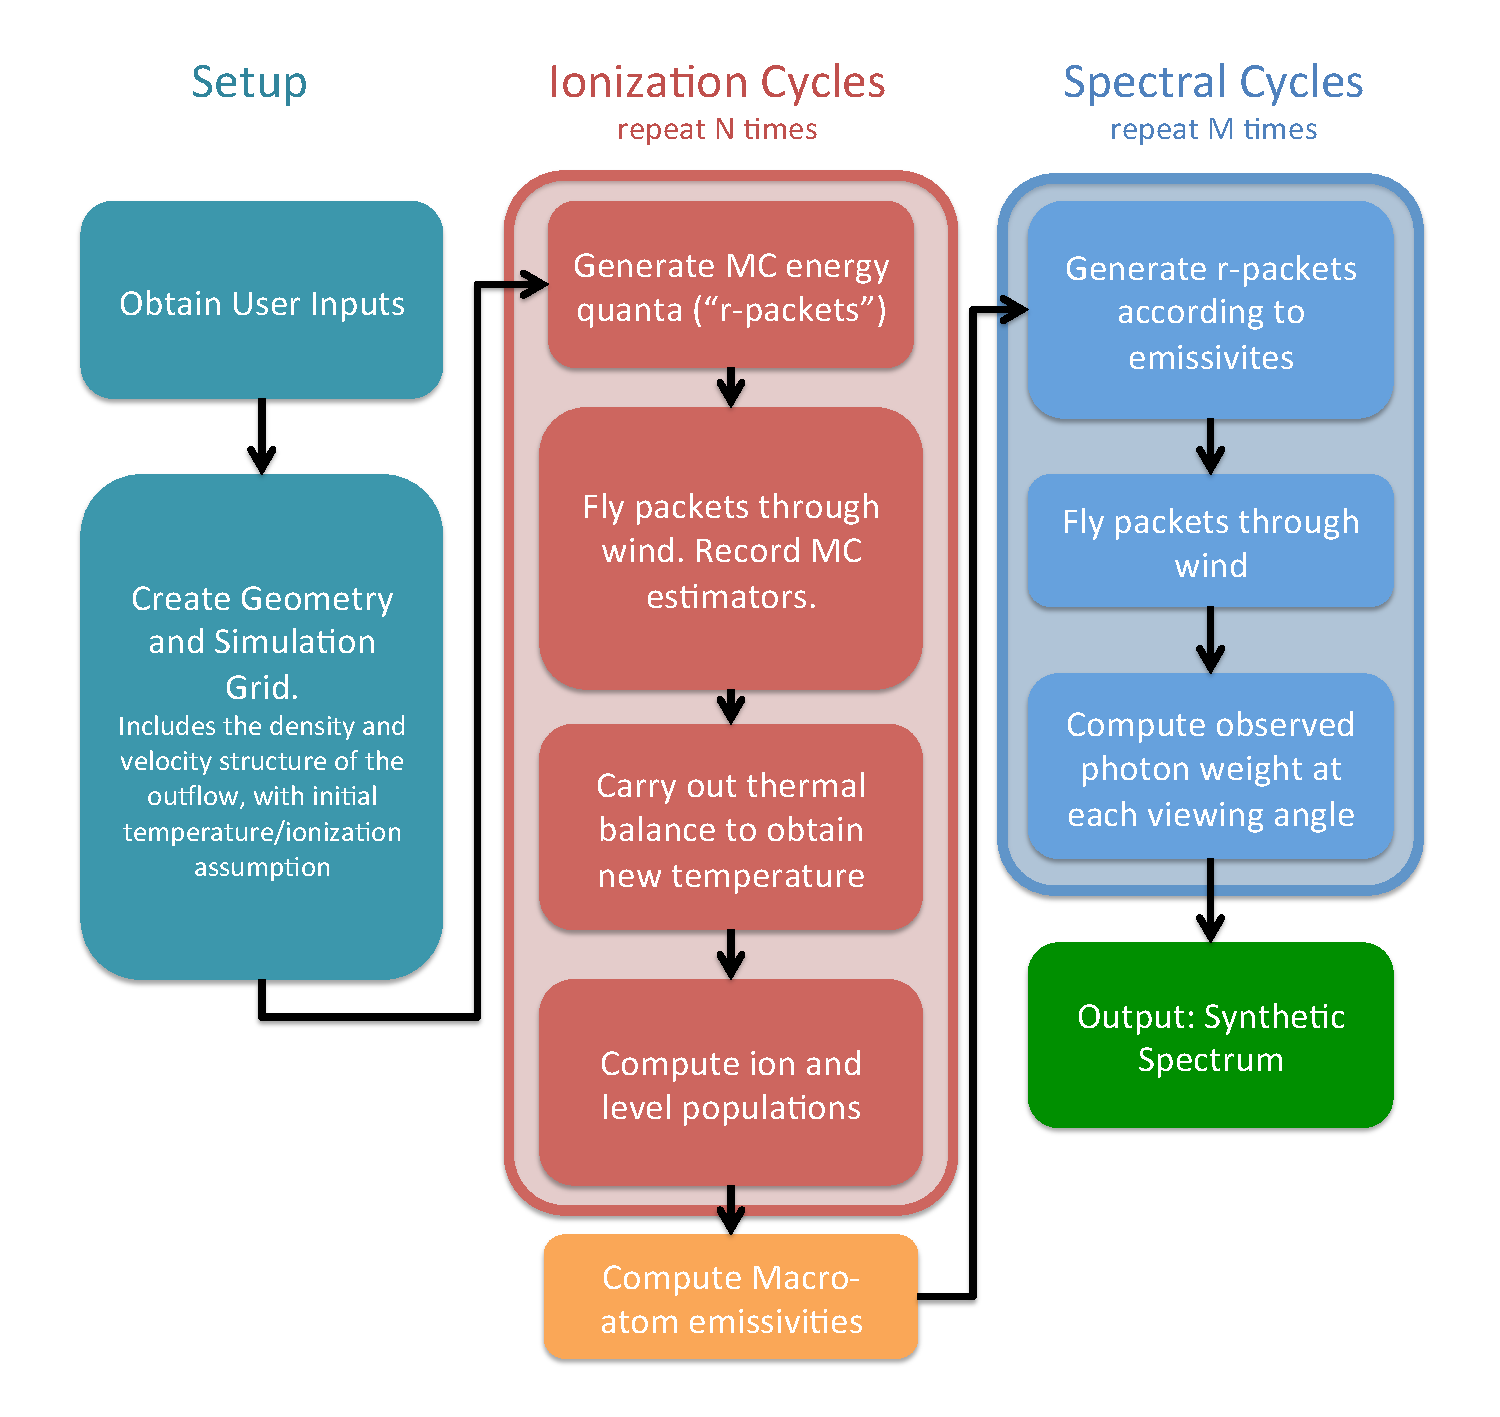
\includegraphics[width=1.0\textwidth]{figures/03-radtrans/flowchart.pdf}
\caption
{
A flowchart showing the basic operation of \py.
} 
\label{fig:flowchart}
\end{figure}

\py\ operates in three distinct stages, shown in figure~\ref{fig:flowchart}. 
First, the user specifies the photon sources,
geometry and kinematics of the system, normally with a similar parameterisation
to the SV93 model described in section~\ref{sec:sv93_model}. 
The code can operate with a number of different coordinate systems 
(1D, spherical polar, cylindrical), but in this work I use only cylindrical coordinates.
In this case, the outflow is discretised into a $n_x \times n_z$ logarithmic grid with 
user-specified dimensions. The co-ordinates, $(x_i, z_i$), 
of the corner of the $i$th cell are then given by
\begin{align}
x_i &= L_{x}~10^{(i-1)\frac{\log (R_{\mathrm{max}} / L_{x})}{n_x}},\\
z_i &= L_{z}~10^{(i-1)\frac{\log (R_{\mathrm{max}} / L_{z})}{n_z}},
\end{align}
where $L_x$ and $L_z$ are appropriately chosen (but hardwired) scale lengths, and $R_{\mathrm{max}}$ 
is the extent of the simulation domain.
From these co-ordinates the poloidal distance can be calculated and
the velocity set according to equation~\ref{eq:v_law}. The density
is then calculated from equation~\ref{eq:rho_rz}. An initial temperature,
$T_{\mathrm{init}}$ is set by the user. The ionization fractions throughout
the wind are then initiated to Saha (LTE) abundances at $T_{\mathrm{init}}$, and the level 
populations are initially set according to the Boltzmann formula.

Once the basic setup process has been carried out, the ionization state,
level populations and temperature structure are calculated.
This is done via an iterative process, by transporting several populations of 
Monte Carlo energy quanta (`photons' or `$r$-packets') through the outflow.
This process is repeated until the code converges. 
In each of these iterations (`ionization cycles'), the code records estimators that 
characterize the radiation field in each grid cell. At the end 
of each ionization cycle, a new electron temperature is calculated
that more closely balances heating and cooling in the 
plasma. The radiative estimators and updated electron
temperature are then used to revise the ionization state of the wind,
and a new ionization cycle is started. The process is repeated until
heating and cooling are balanced throughout the wind (see sections~\ref{sec:heating_cooling}
and \ref{sec:convergence}). 

This converged model provides the basis for the second set of
iterations (`spectral cycles'; section~\ref{sec:spectral_cycles}), 
in which the code computes the synthetic spectrum based on the 
MC estimators recorded during the ionization cycles. 
The emergent spectrum over the desired spectral range is synthesized by 
tracking populations of energy packets through the wind and recording 
the escaping energy packets for
a number of user-specified viewing angles.  In the ensuing sections,
I will describe each of the above steps in more detail, particularly
with regards to the macro-atom mode of operation (section~\ref{sec:matoms}).


% \py\ is designed to operate in a number of different
% regimes, both in terms of the scale of the system and in terms of the
% characteristics of the underlying radiation field.
% It was originally developed by LK02 in order to model the UV spectra
% of CVs with a simple biconical disc wind model. SDL05
% \nocite{simmacro2005} used the code to model Brackett
% and Pfund line profiles of H in young-stellar objects (YSOs). As part
% of this effort, they implemented a `macro-atom' mode (see below) in
% order to correctly treat H recombination lines with
% \py. Finally, H13 used \py\ to model broad absorption line (BAL) QSOs. For
% this application, an improved treatment of ionization was implemented,
% so that the code is now capable of dealing with arbitrary
% photo-ionizing SEDs, including non-thermal and multi-component ones. 
\subsection{Radiation Packets}
\label{sec:packets}
Every energy packet in the simulation starts out as a radiation packet generated
from one of $N_S$ photon sources. To ensure that the frequency distribution
of photons is adequately sampled in important frequency regimes, 
{\em stratified sampling} is used. A specified fraction, $f_i$,
of photons must emerge each band $i$, whose frequency boundaries
can be adapted for the astrophysical situation considered. 
The weight, $w_i$, of the radiation packets in a given energy band with boundaries
$\nu_i$ and $\nu_{i+1}$ is then given by
\begin{equation}
w_i = \frac{\sum_j^{N_S} \int_{\nu_i}^{\nu_{i+1}} L_{\nu,j}~d\nu}{f_i~N_p},
\end{equation}
where $N_p$ is the total number of photons desired, 
and $L_{\nu,j}$ is the monochromatic 
luminosity of photon source $j$. 
The frequency of photons is calculated by constructing a 
cumulative distribution function (CDF), $f_{C,i}(\nu)$,
from the spectral energy distribution in each band $i$: 
\begin{equation}
f_{C,i} (\nu) = 
\frac{\int_{\nu_i}^{\nu} L_\nu~d\nu}
{\int_{\nu_i}^{\nu_{i+1}} L_\nu~d\nu} ~.
\end{equation}
A photon frequency can then be generated by cycling through the bands. In each band,
a random number is chosen between 0 and 1, and the frequency is 
then selected by interpolating on the sampled CDF. This process is repeated until 
each band has the specified number of photons, with the packet
weights adjusted accordingly.

\py\ can operate in two modes concerning the approach to energy packets. 
In the original mode described by LK02, continuum processes attenuate 
the weight of the radiation packets. This attenuation is accounted for 
by including the wind as an additional photon source.
In the second mode, energy packets are indivisible and strict radiative equilibrium is
enforced. From here on I will only be discussing this indivisible packet scheme, 
as it is required in order to be able to use macro-atoms to accurately
treat recombination in H and He.

\subsection{Radiative Transfer Procedure}

\label{sec:rt_procedure}

As a photon travels through a plasma, it has a finite probability
of interacting with free or bound electrons and undergoing a scattering
or absorption event. In order to deal with this in a Monte Carlo sense, a random optical 
depth is generated before an $r$-packet is moved,
\begin{equation}
\tau_R = - \ln (1 - {\cal Z}),
\end{equation}
where ${\cal Z}$ is a random number between 0 and 1. 
The $r$-packet is then gradually transported through a given cell. 
As it moves, the optical depth, $\tau^\prime$, it experiences
is incremented continuously, representing continuum processes. When the $r$-packet comes
into resonance with a line, according to equation~\ref{eq:resonance},
the Sobolev optical depth is calculated from equation~\ref{eq:tau_sob} and added to 
$\tau^\prime$. This process is illustrated in Fig.~\ref{fig:scatter_ml93} and
continues until $\tau^\prime \geq \tau_R$ or the $r$-packet leaves the cell. If the
photon leaves the cell, the values of $\tau_R$ and $\tau^\prime$ are preserved,
and the process continues using the conditions in the new cell. If 
$\tau^\prime \geq \tau_R$, then an interaction with the plasma has occurred, and
the process governing this interaction must be identified. This is done by
randomly picking an interaction process in proportion with their contributions
to $\tau^\prime$. If the process is an electron scatter then a new, isotropic
direction is generated for the $r$-packet. Otherwise, the packet must
interact with either the thermal pool or the excitation energy of the plasma.

\begin{figure}
\centering
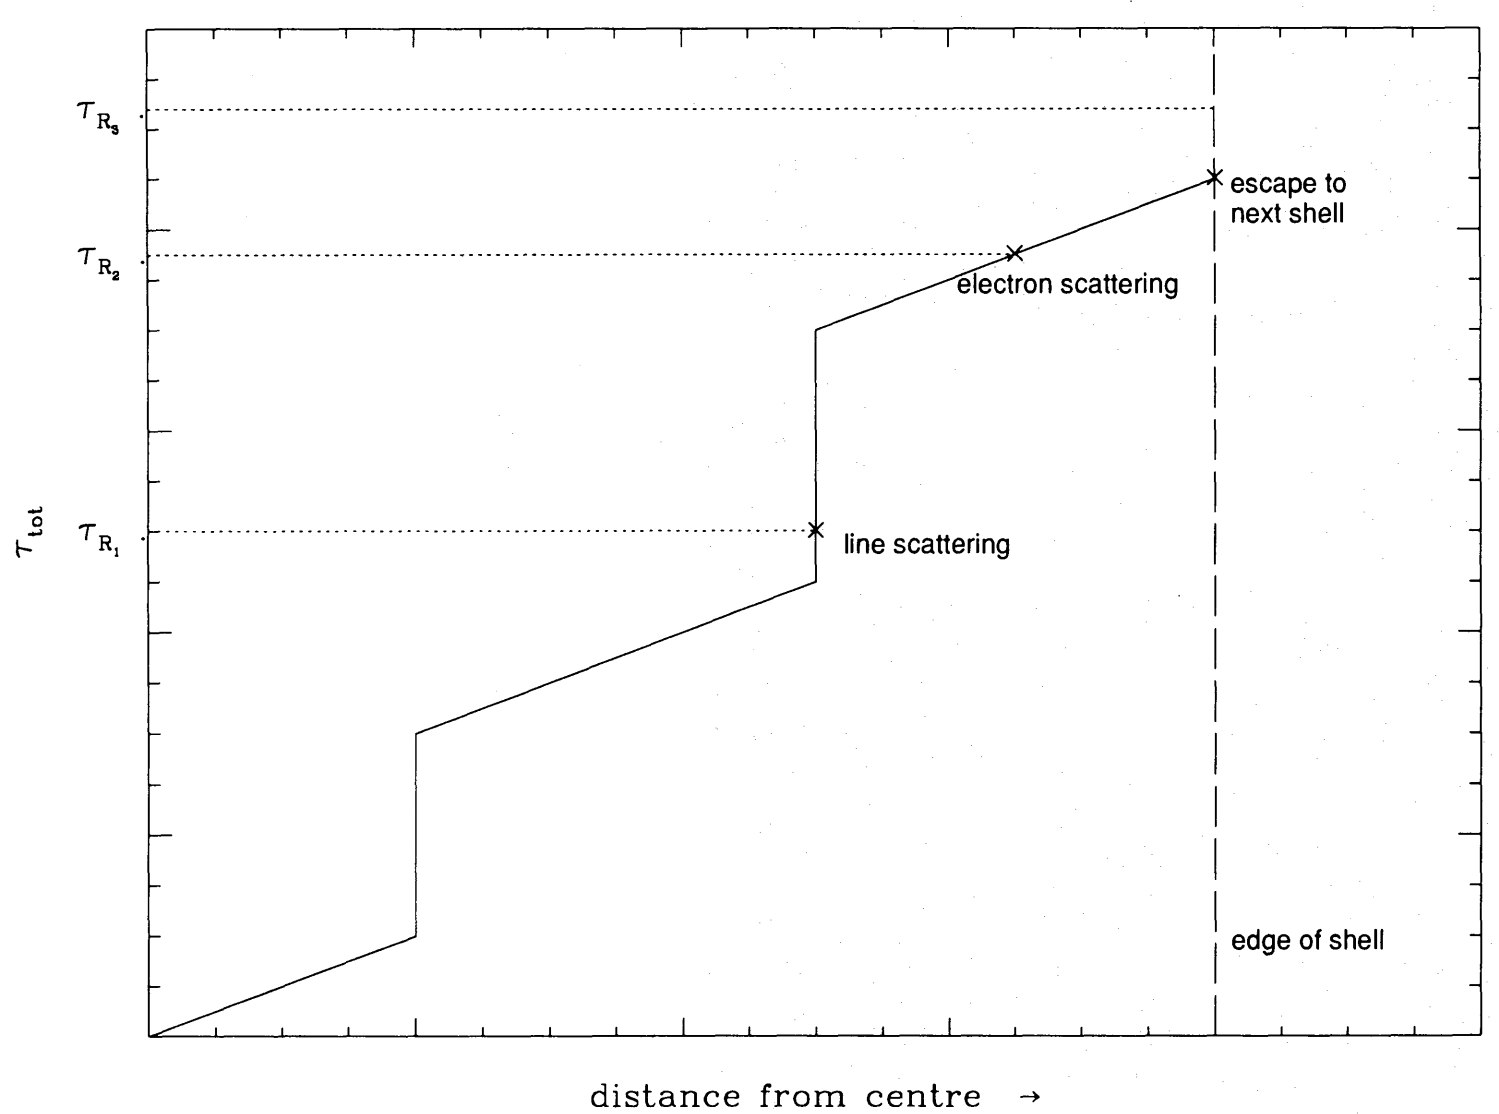
\includegraphics[width=0.7\textwidth]{figures/03-radtrans/tau_scat.png}
\caption
[The process of choosing a scattering location in a cell.]
{
{\sl Credit: Mazzali \& Lucy 1993}. 
The process of choosing a scattering location in a cell.
} 
\label{fig:scatter_ml93}
\end{figure}

\subsubsection{Continuum Opacities}

In order to calculate $\tau^\prime$ in the above approach, we need
to know the opacities that will contribute to it. An opacity 
at a given frequency, $\kappa(\nu)$,
is related to an optical depth, $\tau(\nu)$, by
\begin{equation}
\tau(\nu) = \kappa(\nu)~\Delta s,
\end{equation}
where $\Delta s$ is the distance moved by the photon. The bound-free
opacity is calculated from a sum over photoionization cross-sections (bfjumps),
such that
\begin{equation}
\kappa_{bf} = \sum_{j\kappa}^{\mathrm{bfjumps}} \sigma_{j\kappa} (\nu) n_j.
\end{equation}
The free-free emission coefficient for an individual ion $i$ of charge $Z_i$ 
is \citep{gayet1970}
\begin{equation}
j_{ff,i} (\nu) = \bar{g}_{ff}\frac{8 Z_i^2 q_e^6}{3m_e^2 c^3}
\left( \frac{2\pi m_e}{3 k T_e} \right)^{1/2}
N_i n_e \exp(-h\nu/kT_e),
\label{eq:jff} 
\end{equation}
where $\bar{g}_{ff}$ is the mean free-free Gaunt factor and formally
depends on both frequency and temperature.
The free-free opacity is calculated from Kirchhoff's law, 
\begin{equation}
\kappa_{ff, i}(\nu) = \frac{j_{ff,i} (\nu)}{B_\nu (T_e)}.
\end{equation}
% which gives
% \begin{equation}
% \kappa_{ff, i}(\nu) = \bar{g}_{ff} n_e N_i \frac{4}{3} \left(\frac{2\pi}{3}\right)^{1/2}~
% \frac{Z_i^2 q_e^6}{m_e^2 hc} \left(\frac{m_e}{kT_e}\right)^{1/2}~
%  \nu^{-3} [1 - \exp(-h\nu/kT_e)].
% \end{equation}
The electron scattering opacity is 
\begin{equation}
\kappa_{es} = \sigma_T n_e.
\end{equation}
These opacities are all used in the heating and cooling estimators 
introduced in section~\ref{sec:estimators}. In addition the
Compton opacity is required in order to estimate the Compton heating effect on the plasma.
The Compton opacity is given by
\begin{equation}
\kappa_{C} = \sigma_{KN} (\nu) n_e,
\end{equation}
where $\sigma_{KN} (\nu)$ is the cross-section computed 
from the Klein-Nishina formula \citep{klein-nishina}, and unlike $\sigma_T$
is frequency dependent. Compton opacity is not included in the actual radiative transfer 
in the simulations presented in this thesis, but is included in the heating and 
cooling balance (see section~\ref{sec:estimators}).

\subsubsection{Doppler Shifts}

When calculating opacities, the photon frequency must be shifted from
the rest frame of the photon into the rest frame of the plasma.
This shift depends on the before and after directions of the photon. Let us denote
these two directions with unit vectors $\vec{n}_i$ and $\vec{n}_f$, respectively,
and consider a situation when a photon scatters off an electron in a region of the
wind moving at velocity $\vec{v}$.
The final frequency of the photon with initial frequency $\nu_i$ is then 
\begin{equation}
\nu_f = \nu_i ~\frac{1 - (\vec{v} \cdot \vec{n}_i) / c}{1 - (\vec{v} \cdot \vec{n}_f) / c}.
\end{equation}
In the case of a resonance scatter with line transition $u \rightarrow j$, the 
new frequency is
\begin{equation}
\nu_f = \frac{\nu_{uj}}{1 - (\vec{v} \cdot \vec{n}_f) / c}.
\end{equation}
When we consider that the resonant point is chosen according to 
equation~\ref{eq:resonance} and that $v=\vec{v} \cdot \vec{n}_f$ in this case,
it is clear that the above two equations are equivalent.


\subsubsection{Choosing Packet Directions}

The last variable, in addition to $w_i$ and $\nu$, needed to define a 
radiation packet is the direction of travel.
In the case of isotropic emission, the direction of a photon packet
is chosen so that the probability of emission in each bin of solid
angle is the same. It follows that 
\begin{equation}
p(\Omega)d\Omega \propto \cos \theta \sin \theta d\theta d\phi,
\end{equation}
where the angles are in polar coordinates and relative to the local
outward normal. For a spherical emitting source, such as 
a star, one must first generate a location on the star's surface
and then calculate the photon direction relative to the normal at the point.
For emission from optically thick surfaces the above equation can be modified
to include linear limb darkening, $\eta(\theta)$:
\begin{equation}
p(\theta, \phi) d\theta d\phi = \eta(\theta) \cos \theta \sin \theta d\theta d\phi.
\end{equation}
The Eddington approximation is usually adopted in the code, so that $\eta(\theta)$
is given by
\begin{equation}
\eta(\theta) = a (1 - \frac{3}{2} \cos \theta).
\end{equation}
The constant $a$ is normalised such that the total probability
sums to $1$. Whenever a radiation packet undergoes an electron scatter,
the new direction is chosen to be isotropic. However,
when the photon is a line photon, the new direction is chosen
according to a line trapping model, which samples a probability 
distribution according to the Sobolev escape probability in different 
directions. 


%%%%%%%%%%%%%%%%%%%%%%%%%%%%%
%MACRO ATOMS
%%%%%%%%%%%%%%%%%%%%%%%%%%%%%

%%%%%%%%%%%%%%%%%%%%%%%%%%%%%
%%%%%%%%%%%%%%%%%%%%%%%%%%%%%
% MACRO ATOMS
%%%%%%%%%%%%%%%%%%%%%%%%%%%%%
%%%%%%%%%%%%%%%%%%%%%%%%%%%%%

\section{Macro-atoms}
\label{sec:matoms}
{\sl The macro-atom scheme was created by Leon Lucy and is outlined in 
his 2002/03 papers. It was implemented in \py\ by Stuart Sim, initially
for the study of recombination lines in YSOs (SDL05).
}

\citet[][hereafter L02, L03]{lucy2002, lucy2003}
has shown that it is possible to calculate the emissivity of a gas in
statistical equilibrium without approximation for problems with large departures
from LTE.
His `macro-atom'\index{macro-atom} scheme allows for all possible transition paths from a given level,
dispensing with the two-level approximation, and
provides a full non-LTE solution\index{LTE}
for the level populations based on Monte Carlo estimators. The macro-atom
technique has already been used to model Wolf-Rayet star\index{Wolf-Rayet star}
winds \citep{sim2004}, AGN disc winds \citep{simlong2008, tatum2012},\index{YSO}\index{Supernova}
supernovae \citep{kromersim2009, kerzendorfsim} and YSOs (SDL05). A full 
description of the approach can be found in L02 and L03.\index{stellar wind}

Understanding macro-atoms requires something of a philosophical shift.
Normally MCRT is described in the most intuitive way- that is, we imagine
real photons striking atoms and either scattering or imparting energy to a 
bound electron. With Lucy's scheme we instead 
reimagine the MC quanta as packets of quantised energy flow, 
so that the scheme becomes a purely
{\em statistical} one. The amount of time a given energy quantum spends in a specific atomic
level or thermal pool is then somewhat analogous to the absolute energy 
contained therein.

Following L02, let us consider an atomic species interacting with a radiation field.
If the quantity $\epsilon_j$ represents the ionization plus excitation energy of 
a level $j$ then the rates at which the level absorbs and emits radiant energy 
are given by
\index{Macro-atoms!Rate equations}
\begin{equation}
 \dot{A}_{j}^{R} = R_{\ellp j} \epsilon_{j \ellp} \;\;\;\;\; {\rm and} \;\;\;
\;\;  \dot{E}_{j}^{R} = R_{j \ellp} \epsilon_{j \ellp} \;\;\; ,
\end{equation}
where $\epsilon_{j \ellp} = \epsilon_j - \epsilon_\ellp$.
Here, I have adopted Lucy's convention, in which the subscript 
$\ellp$ denotes a summation over all lower states ($\ell<j$), and
$\up$ a summation over all upper states ($u>j$).
Similarly, the rates corresponding to {\em kinetic} (collisional)
energy transport can then be written as
\begin{equation}
 \dot{A}_{j}^{C} = C_{\ellp j} \epsilon_{j \ellp} \;\;\;\;\; {\rm and}
\;\;\;
\;\;  \dot{E}_{j}^{C} = C_{j \ellp} \epsilon_{j \ellp} \;\;\; ,
\end{equation}
Let us define ${\cal R}$ as a total rate, such that
${\cal R}_{\ellp j}  = R_{\ellp j} + C_{\ellp j}$.
If we now impose statistical equilibrium\index{statistical equilibrium}
%
\begin{equation}
 ({\cal R}_{\ellp j}-{\cal R}_{j \ellp})+({\cal R}_{\up j}-{\cal R}_{j\up})=0 \;\;\;,
\end{equation}
we obtain 
\begin{eqnarray}
 \dot{E}_{j}^{R}+\dot{E}_{j}^{C}+{\cal R}_{j\up}\epsilon_{j}+
 {\cal R}_{j \ell}\epsilon_{\ellp}  \nonumber \\  
 = \dot{A}_{j}^{R}+\dot{A}_{j}^{C}+{\cal R}_{\up j} \epsilon_{j}
 +{\cal R}_{\ellp j} \epsilon_{\ellp}           .  
 \label{eq:matom_SE}     
\end{eqnarray}
This equation is the starting point for the macro-atom scheme. It shows 
that, when assuming radiative equilibrium, the energy flows through
a system depend only on the transition probabilities and atomic physics
associated with the levels the energy flow interacts with.
By quantising this energy flow into radiant ($r$-) and kinetic ($k$-) packets, 
we can simulate the energy transport through
a plasma discretised into volume elements (``macro-atoms''),
whose associated transition probabilities govern the interaction 
of radiant and kinetic energy with the ionization and excitation energy associated 
with the ions of the plasma.

Although equation~\ref{eq:matom_SE} assumes strict radiative equilibrium,\index{radiative equilibrium}
it is trivial to adjust it to include non-radiative source and sink terms. 
For example, in an expanding parcel of plasma, adiabatic cooling may be 
included with a simple modification to the RHS of equation~\ref{eq:matom_SE}.
\index{adiabatic cooling}


%%%%%%%%%%%%%%%%%%%%%%%%%%%%%
% PROBS
%%%%%%%%%%%%%%%%%%%%%%%%%%%%%

\subsection{Transition Probabilities}

Having interpreted equation~\ref{eq:matom_SE} in a {\em stochastic} way,
we can now construct our Monte Carlo scheme, following L02.
A macro-atom in state $j$ always has a finite probability of `deactivating'
radiatively or collisionally:
\begin{equation}
p_{j}^{R} = \dot{E}_{j}^{R} / D_j \;\;\;\;\; {\rm and} \;\;\;
\;\; p_{j}^{C} = \dot{E}_{j}^{C} / D_j,
\label{eq:deactivate}
\end{equation}
where I have defined
\begin{equation}
D_j =  \dot{E}_{j}^{R}+\dot{E}_{j}^{C}+{\cal R}_{j\up}\epsilon_{j}+
 {\cal R}_{j \ellp}\epsilon_{\ellp} = ({\cal R}_{j\ellp} + {\cal R}_{j\up}) \epsilon_{j}.
\end{equation}
The corresponding jumping probabilities\index{macro-atom!transition probability}, 
which describe the probability
that the macro-atom transitions to a different state while remaining active, 
are given by
\begin{equation}
p_{ju} = {\cal R}_{ju} \epsilon_{j} / D_j \;\;\;\;\; {\rm and} \;\;\;
\;\; p_{jl} = {\cal R}_{jl} \epsilon_{l} / D_j.
\end{equation}
Note that the jumping probability is always proportional to the energy
of the lower level, whereas the emission probability is proportional
to the energy {\em difference} between the levels, as 
$\dot{E}_{j}^{R} = R_{j\ellp} (\epsilon_j - \epsilon_\ellp)$. We can also
trivially show that the probabilities are correctly normalised, as
\begin{align}
p_{j}^{R} + p_{j}^{C} + p_{jl} + p_{ju} &=
(1/D_j) ( {\cal R}_{j\up} \epsilon_{j} + {\cal R}_{j\ellp} \epsilon_{\ellp} +
\dot{E}_{j}^{R} + \dot{E}_{j}^{C}) \\
&= 1. \nonumber
\end{align}

With these transition
probabilities identified, a Monte Carlo calculation can proceed by formulating
the normal statistical equilibrium rate equations that will depend on
the ambient conditions of the plasma. The effect of these ambient conditions
is expressed through the use of Monte Carlo estimators.




%%%%%%%%%%%%%%%%%%%%%%%%%%%%%
% RATES
%%%%%%%%%%%%%%%%%%%%%%%%%%%%%
\subsection{Rate equations}
\label{sec:rate_eq}\index{Monte Carlo!estimator}
The macroscopic transition probabilities above depend on the traditional
rate equations formulated according to statistical equilibrium. 
In the framework of the Sobolev escape probability formalism\index{Sobolev approximation} 
(see section~\ref{sec:sobolev}),\index{radiative excitation}\index{radiative de-excitation}
the bound-bound excitation rate, ${\cal R}_{ju}$, in an ion is given by 
\begin{equation}
{\cal R}_{ju} = B_{ju} n_j J_{\mathrm{est}} \left(1 - \frac{n_j g_u}{n_u g_j} \right) + q_{ju} n_j n_e,
\label{eq:rju}
\end{equation}
where $u$ is now a specific upper level, and $q_{ju}$ is the collisional
rate coefficient (see section~\ref{sec:coll}). The $(1 - n_j g_u/n_u g_j)$ term
is the correction for stimulated emission from equation~\ref{eq:einstein_relations},
and requires that there are no population inversions (see section~\ref{sec:numerical_matom}).
The quantity $J_{\mathrm{est}}$ is the Monte Carlo estimator for the mean intensity 
impinging on the Sobolev region, weighted by an angle-dependent escape probability, 
given by \citep{sim2004}
\begin{equation}
J_{\mathrm{est}} = \frac{c}{4 \pi \nu_{uj} V} \sum_{i}^{\mathrm{photons}} w_i \frac{1 - e^{-\tau_{s,i}}}{\tau_{s,i}} \frac{1}{(dv/ds)_i}.
\end{equation}
Here $w_i$ is the photon weight (in luminosity units), $\nu_{uj}$
is the line frequency, $dv/ds$ is the velocity gradient and
$\tau_s$ is the Sobolev optical depth.
The sum is over all photons that come into resonance with the line,
and thus represents an integral over solid angle.
This is essentially the MC estimator form of $\beta_{uj}\bar{J}_{uj}$, and
reduces to the estimator in equation~20 of L02 
in the limit of homologous flow or symmetric escape probabilities.
The corresponding de-excitation rate is then \index{Sobolev approximation}
\begin{equation}
{\cal R}_{uj} = \beta_{ju} A_{uj} n_u + B_{uj} n_u J_{\mathrm{est}}  +
q_{uj} n_u n_e.
\label{eq:ruj}
\end{equation}
The photoionization and collisional ionization rates
between a lower level, $l$, and the continuum level $\kappa$ 
(or, in the case of ions with more than one bound electron, 
the ground state of the upper ion),
$\kappa$, are
\begin{equation}
{\cal R}_{j \kappa}= \gamma_{j\kappa} n_j - \alpha^{st}_{\kappa j} n_\kappa n_e   + q_{j \kappa} n_j n_e.
\label{eq:rjk}
\end{equation}
Here, $q_{j \kappa}$ is the collisional ionization rate coefficient,\index{collisional ionization}
$\gamma_{j \kappa}$ is the photoionization rate\index{photoionization}
from $j \rightarrow \kappa$, and $\alpha^{st}_{\kappa j}$ is the stimulated recombination
coefficient. This is included as a negative photoionization term rather 
than a positive recombination term as in L03, which requires that there are
no population inversions (see section~\ref{sec:numerical_matom}). 
The corresponding recombination rate is given by\index{recombination}
\begin{equation}
{\cal R}_{\kappa j} = \alpha_{\kappa j} n_{\kappa} n_e + q_{\kappa j}
n_\kappa n_e, \\
\end{equation}
where $\alpha_{\kappa l}$ is the radiative recombination coefficient
to level $l$, and is given by 
\begin{equation}
\alpha_{\kappa j} = 4\pi \left( \frac{n_j}{n_e n_\kappa} \right)^*_{T_e} \int^\infty_{\nu_0} 
\frac{\sigma_{j\kappa} (\nu)}{h \nu} \frac{2 h \nu^3}{c^2} 
\exp \left( \frac{- h \nu}{k T_e} \right) d\nu.
\label{eq:alpha_sp}
\end{equation}
This treatment means that radiative and collisional
rates to and from all levels can be considered when calculating the
ionization state, level populations and transition probabilities, 
although ionization directly to excited levels of the upper ion is 
neglected.\index{level population}

\subsubsection{Collision Strengths}
\label{sec:coll}

The bound-bound collisional de-excitation rate coefficient, $q_{uj}$, is calculated from the
\cite{vanregemorter} approximation, given by\index{bound-bound collision strength}
\begin{equation}
q_{uj} = \bar{g} f_{ju}\frac{8.629\times10^{-6}}{g_u T_e^{1/2}}
\frac{8 \pi}{\sqrt{3}}~\frac{g_j}{g_u} \frac{\nu_{\mathrm{Ryd}}}{\nu_{uj}}
\label{eq:vanregemorter}
\end{equation}
where $\lambda_{uj}$ is the wavelength of the transition, $\nu_{\mathrm{Ryd}}$
is the frequency at $13.6$~eV and $\bar{g}$ is 
an effective gaunt factor of order unity.
The inverse rate is calculated by considering detailed balance, 
such that
\begin{equation}
q_{ju} = q_{uj} \frac{g_u}{g_j} \exp \left( \frac{-h \nu_{uj}}{k T_e} \right).
\label{eq:vanregemorter2}
\end{equation}\index{bound-bound collision strength}
Using equation~\ref{eq:vanregemorter} means that collisions between radiatively
forbidden transitions are not taken into account when one 
splits levels into $l$- and $s$-subshells, as well
as principal quantum number, $n$ (as done with He~\textsc{i}; 
for the CV models in chapter 4). Although this approximation is, in general, 
a poor one, the effect is second order in the physical 
regime where recombination lines are formed in the models presented here 
(see section~\ref{sec:coll_bl}).\index{van Regemorter approximation} 

The bound-free collision strengths are calculated using equation~5.79 of
\cite{mihalas}. The collisional ionization rate coefficient is\index{collisional ionization}
\begin{equation}
q_{j\kappa} = 1.55 \times 10^{-13} n_e~\bar{g}_{i}~\sigma_{j\kappa} (\nu_{\kappa j})~
\frac{h \nu_{\kappa j}}{k T_e^{3/2}}
\exp \left( \frac{- h \nu_{\kappa j}}{k T_e} \right),
\label{eq:qioniz}
\end{equation}
where $\sigma_{j\kappa} (\nu_{\kappa j})$ is the photoionization cross-section 
at the threshold energy.
The effective gaunt factor for ion $i$, $\bar{g}_{i}$, is approximately
equal to $0.1,0.2,0.3$ for $Z=1,2$ and $>2$, respectively,
where $Z$ is the atomic number. Note that the use of this estimator
implies a $\nu^{-3}$ shape to the photoionization cross-section,
which is only strictly true for for hydrogenic ions.
The collisional (three-body) recombination rate is found using the Saha equation
and given by\index{collisional recombination}\index{Saha equation}
\begin{equation}
q_{\kappa j} = q_{j\kappa} \left( \frac{n_j}{n_e n_\kappa} \right)^*_{T_e}.
\label{eq:qrecomb}
\end{equation}
For numerical reasons, the above two expressions are combined in \py\ where 
possible, in order to avoid multiplying two exponentials.
\index{recombination}




%%%%%%%%%%%%%%%%%%%%%%%%%%%%%
%ESTIMATORS
%%%%%%%%%%%%%%%%%%%%%%%%%%%%%
\subsection{Macro-atom estimators}
\label{sec:estimators}
In order to solve the above rate equations and compute the transition 
probabilities, it is necessary to construct estimators for the various properties
of the radiation field that appear in the macro-atom rate equations. This is done
by converting integrals over the radiation field into summations over 
$r$-packets passing through a cell. This represents the stochastic nature of
a MC simulation and is by no means unique to the macro-atom formalism.
The first step is to apply the energy-density argument of \cite{lucy1999radeq},
which gives, for a time-independent code\index{Monte Carlo!estimator}
\begin{equation}
J_\nu~d\nu = \frac{1}{4\pi}\frac{1}{V} \sum_{d\nu} w_i \Delta s,
\end{equation}
\index{mean intensity}
where the summation is over all photons between $(\nu, \nu+d\nu)$. This allows
the formulation of estimators in a MC sense, rather than in integral form. 

\subsubsection{Bound-free estimators}
The estimator for the photoionization rate is\index{photoionization rate}\index{photoionization}
\begin{equation}
\gamma_{j\kappa} = \frac{1}{V} \sum_i^{\mathrm{photons}} 
\frac{w_i~\sigma_{j\kappa}({\nu})}{h \nu}~\Delta s
\end{equation}
and that for the stimulated recombination\index{stimulated recombination} rate is
\begin{equation}
\alpha_{\kappa j}^{st} =\left( \frac{n_j}{n_e n_\kappa} \right)^*_{T_e}
\frac{1}{V} \sum_i^{\mathrm{photons}} 
\frac{w_i~\sigma_{j\kappa}({\nu})}{h \nu}
~\exp(-h\nu/kT_e)~\Delta s,
\end{equation}
where $\sigma_{j\kappa} (\nu)$ is the photoionization cross-section for this transition.
We also need to define modified rate coefficients to represent
the rates at which bound-free transitions add energy to, and remove energy from, 
the radiation field. These are required for photoionization, 
spontaneous recombination and stimulated recombination and are given by\index{recombination}

\begin{equation}
\gamma^E_{j\kappa} = \frac{1}{V} \sum_i^{\mathrm{photons}} 
\frac{w_i~\sigma_{j\kappa}}{h \nu_{\kappa j}}~\Delta s, 
\end{equation}

\begin{equation}
\alpha^E_{\kappa j} = 4\pi \left( \frac{n_j}{n_e n_\kappa} \right)^*_{T_e}
 \int^\infty_{\nu_{\kappa j}} 
\frac{\sigma_{j \kappa}(\nu)}{h \nu_{\kappa j}} \frac{2 h \nu^3}{c^2} 
\exp \left( \frac{- h \nu}{k T_e} \right) d\nu,
\end{equation}

\begin{equation}
\alpha_{\kappa j}^{st,E} = \left( \frac{n_j}{n_e n_\kappa} \right)^*_{T_e}
\frac{1}{V} \sum_i^{\mathrm{photons}}
\frac{w_i~\sigma_{j\kappa}({\nu})}{h \nu_{\kappa j}}
~\exp(-h\nu/kT_e)~\Delta s.
\end{equation}
The rate at which recombinations convert
thermal {\em and} ionization energy into radiant energy is then
$\alpha^E h\nu_{\kappa j} n_\kappa n_e$, where $h \nu_{\kappa j}$
the energy difference between the continuum state $\kappa$ and 
the level $j$ the electron is recombining into. 
The amount of this energy which is removed from the thermal pool
therefore given by the estimator\index{recombination}
\begin{equation}
\cc_{bf} = \sum_{j\kappa}^{\mathrm{bfjumps}} 
\left[ (\alpha^E_{\kappa j} + \alpha^{st,E}_{\kappa j} - \alpha_{\kappa j} - \alpha^{st}_{\kappa j}) 
n_{\kappa} + 
q_{j\kappa} n_j \right]
n_e h\nu_{\kappa j} V,
\end{equation}
where the sum is over all the macro-atom bound-free transitions ($j\rightarrow\kappa$) 
in the simulation, set by
the number of photoionization cross-sections. 
For bound-free heating\index{bound-free heating}, a similar expression can be derived. The rate at which
a level $j$ absorbs energy by bound-free 
transitions is given by $\gamma^E_{j\kappa} h\nu_{\kappa j} n_\kappa n_e$,
of which $\gamma_{j\kappa} h \nu_{\kappa j} n_l$ goes into ionization energy, leaving 
\begin{equation}
\hh_{bf} = \sum_{j\kappa}^{\mathrm{bfjumps}} \left[ (\gamma^E_{\kappa j} - \gamma_{\kappa j}) n_j + n_\kappa n_e^2 q_{\kappa j} \right] h \nu_{\kappa j} V
\end{equation}
as the rate at which radiant energy heats the plasma via bound-free transitions.


\subsubsection{Bound-bound estimators}
The heating and cooling rates for macro-atom bound-bound transitions are the rates of
collisional excitations and de-excitations
- i.e. the rate at which thermal energy is converted into
bound-bound excitation energy and vice versa.
These heating and cooling rate estimators are:\index{bound-bound heating}\index{bound-bound cooling}

\begin{equation}
\hh_{bb} = \sum_{ju}^{\mathrm{lines}} q_{uj} n_u n_e h \nu_{uj} V,
\end{equation}


\begin{equation}
\cc_{bb} = \sum_{ju}^{\mathrm{lines}} q_{ju} n_j n_e h \nu_{uj} V.
\end{equation}

\subsubsection{Other heating and cooling estimators}
Although I have now defined the estimators required to calculate the 
transition probabilities, level populations, heating rates and cooling rates in macro-atoms, 
there are still a number of heating and cooling mechanisms that do not involve macro-atoms. 

The free-free cooling estimator is calculated from the emission coefficient
in equation~\ref{eq:jff},\index{free-free cooling}
\begin{equation}
\cc_{ff} = V \sum_i^{\mathrm{ions}} \int \frac{j_{ff,i}(\nu)}{4\pi} d\nu,
\end{equation}
where the integral is over all frequencies included in the simulation,
and the sum is also over all ions included in the simulation.
The corresponding heating rate is then\index{free-free heating}
\begin{equation}
\hh_{ff} = \sum_i^{\mathrm{photons}} w_i \kappa_{ff} \Delta s.
\end{equation}
Compton heating and cooling is included in the thermal balance and as
$(r\rightarrow k)$ and $(k\rightarrow r)$ transitions:\index{Compton heating}
\begin{equation}
\cc_{\mathrm{comp}} = 16 \pi \sigma_T V J \frac{k T_e}{m_e c^2},
\end{equation}
\begin{equation}
\hh_{\mathrm{comp}} = n_e \sum_i^{\mathrm{photons}} \frac{h\nu}{m_e c^2} w_i \kappa_{C}\Delta s,
\end{equation}
where the estimator for the frequency-integrated mean intensity is\index{mean intensity}
\begin{equation}
J = \frac{1}{4\pi V} \sum_i^{\mathrm{photons}} w_i \Delta s.
\label{eq:j}
\end{equation}
Induced Compton heating is then given by \citep{cloudy2013}\index{Compton heating!induced}
\begin{equation}
\hh_{\mathrm{ind~comp}} = n_e \sum_i^{\mathrm{photons}} \frac{J_\nu c^2}{h \nu^3} \frac{h\nu}{m_e c^2} 
w_i \kappa_{C} \Delta s,
\end{equation}
where $J_\nu c^2/h \nu^3$ represents the
photon occupation number, and $J_\nu$ is either 
calculated from the spectral model
described in section~\ref{sec:simple_ionization} or from a dilute blackbody.
The adiabatic cooling rate is derived by considering the $PdV$ work done by the flow
and is given by\index{adiabatic cooling}
\begin{equation}
\cc_{a} = k T_e V (\nabla \cdot v) \left(n_e + \sum\limits_{i=1}^{\mathrm{ions}} N_i\right),
\end{equation}
where $\nabla \cdot v$ is the divergence of the 
velocity field at the centre of the cell. The sum is over all ions 
included in the simulation.

\noindent

%%%%%%%%%%%%%%%%%%%%%%%%%%%%%
% K PACKETS
%%%%%%%%%%%%%%%%%%%%%%%%%%%%%
\subsection{$k$-packets}\index{$k$-packet}
$k$-packets represent quantised kinetic or thermal energy, and any interaction
chain involving a $k$-packet thus represents interaction with the thermal
pool of ions and electrons. $k$-packets can be produced either directly
via a continuum heating process ($r \rightarrow k$), 
or by the collisional de-activation of a macro-atom 
($r \rightarrow \ldots \rightarrow A^* \rightarrow k$) in accordance with
equation~\ref{eq:deactivate}. 

Once they are produced, $k$-packets never move, as they represent the quantised
thermal energy flow in a finite volume element. Hence, when they are produced,
their destruction path is decided according to the different cooling mechanisms
in the plasma. A $k$-packet then has a probability of being destroyed by process $i$ that
is given by
\begin{equation}
p_{i,\mathrm{destruct}} = \cc_i / (\cc_{bf} + \cc_{ff} + \cc_{bb} + \cc_{\mathrm{comp}} + \cc_a).
\end{equation}
Note that only adiabatic cooling leads to an actual destruction of the energy packet,
as a departure from radiative equilibrium. All other processes will lead to the 
creation of an active macro-atom or an $r$-packet.\index{adiabatic cooling}


%%%%%%%%%%%%%%%%%%%%%%%%%%%%%
% FLOWCHART
%%%%%%%%%%%%%%%%%%%%%%%%%%%%%

\subsection{Putting it All Together}

I have now defined all quantities needed to write down the transition 
probabilities in a macro-atom simulation. Fig.~\ref{fig:flow_matom}
shows the decision tree traversed by an energy packet in the simulation,
showing the complicated set of interactions it can undergo each time it 
scatters.\index{macro-atom}

\begin{figure}
\centering
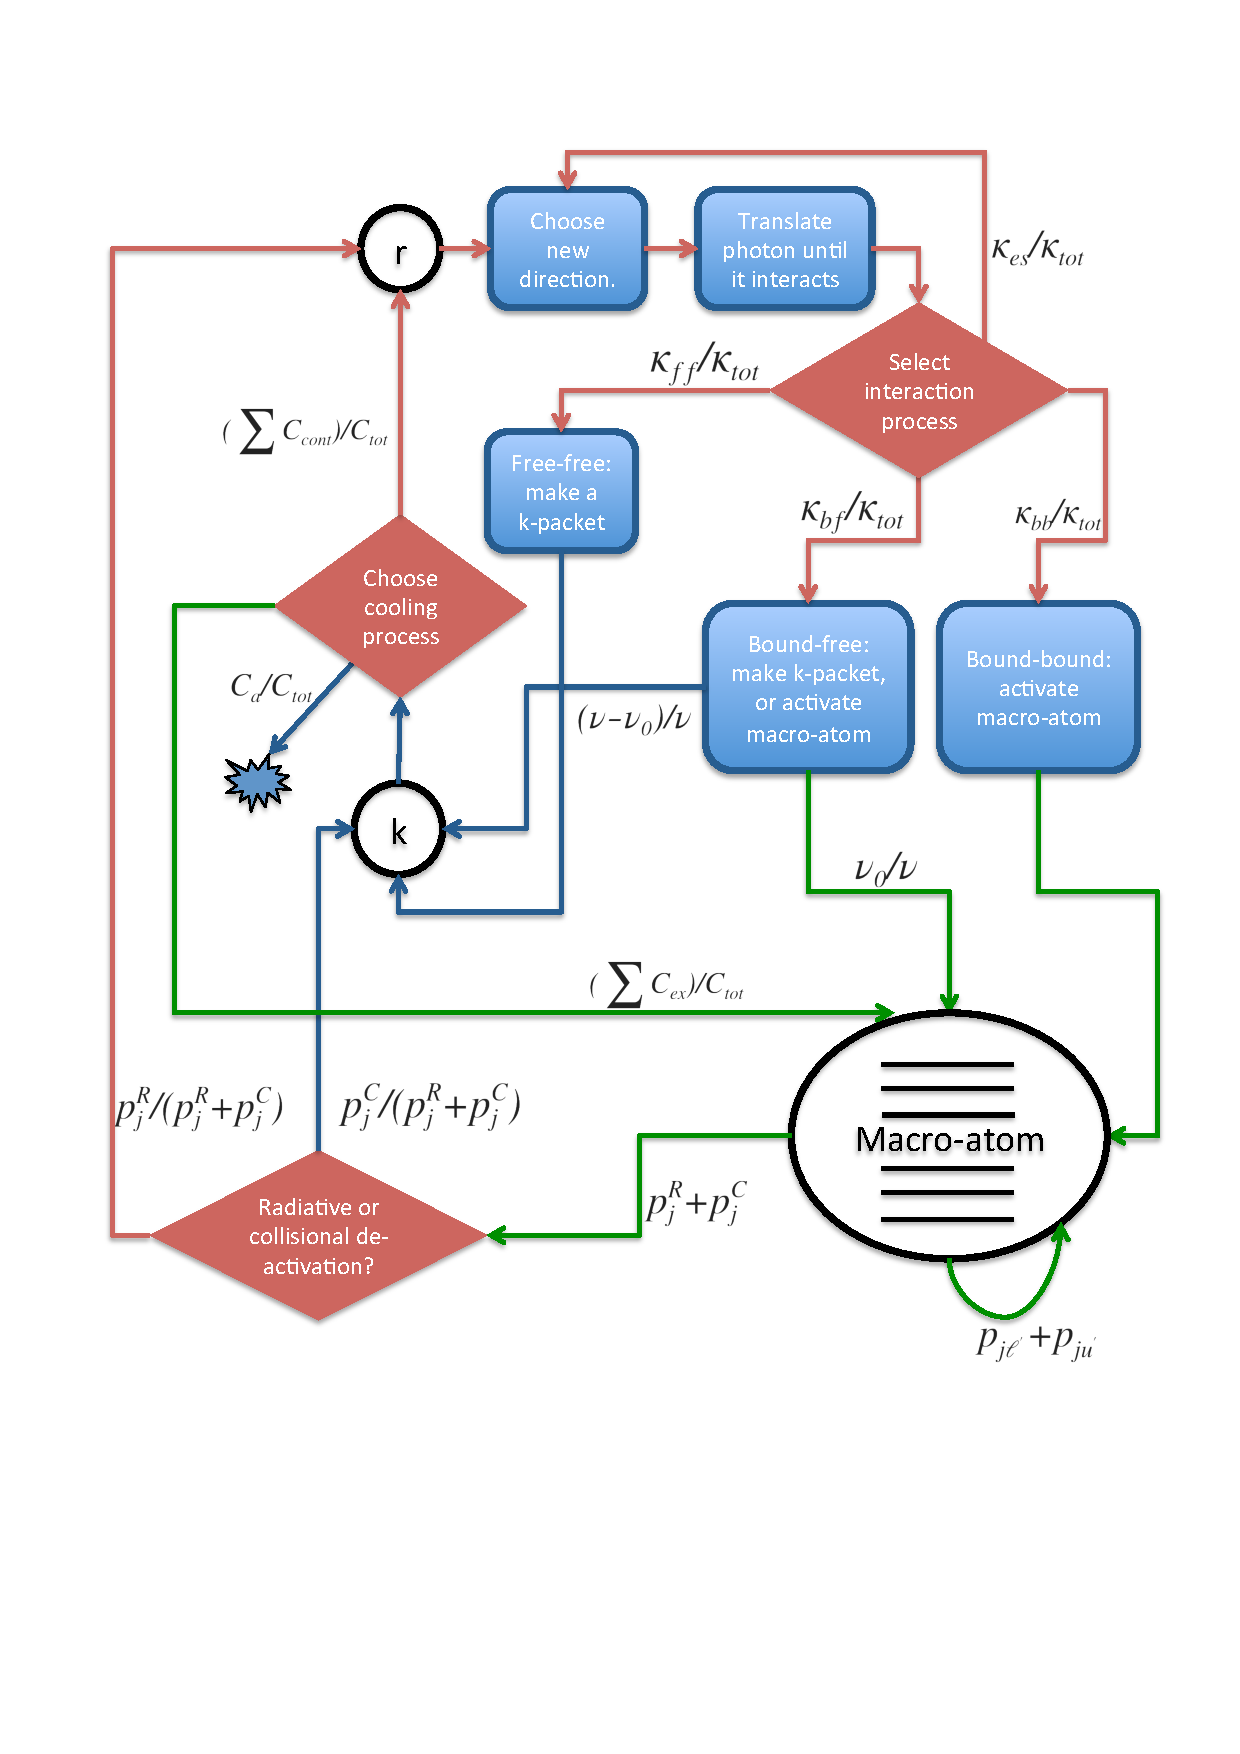
\includegraphics[width=1.0\textwidth, clip=true, trim=0 2.6in 0in 0in ]{figures/03-radtrans/matom_flow_ca.pdf}
\caption
[The decision tree traversed by an energy packet 
in macro-atom mode.]
{
The decision tree traversed by an energy packet 
in macro-atom mode, depicting the interaction
between radiation ($r$-packets), the thermal pool ($k$-packets), and ionization
and ionization/excitation energy (macro-atoms). 
The probabilities at each decision point are 
marked, and are defined in the text. The red, blue and green coloured arrows
represent radiant, kinetic and ionization/excitation energy respectively.
The symbols are defined in the text, except ${\cal C}_{\mathrm{cont}}$ and 
${\cal C}_{\mathrm{ex}}$ which refer to cooling contributions to radiative and excitation 
energy respectively.
} 
\label{fig:flow_matom}
\end{figure}

%% XXX CHECK THIS.


%%%%%%%%%%%%%%%%%%%%%%%%%%%%%
% POPS
%%%%%%%%%%%%%%%%%%%%%%%%%%%%%


\subsection{Ionization Fractions and Level Populations}
\label{sec:matom_pops}
In section~\ref{sec:lte} I described how it is possible to calculate the
ionization and excitation of a plasma under LTE or dilute approximations.
Macro-atoms are not approximated -- their level and ion populations are 
calculated by solving the rate equations formulated in section~\ref{sec:rate_eq}. 
This is done via matrix inversion. For an element with $n$ ions and $m_i$
levels in each ion, we construct a square matrix with dimensions 
$m = \sum_i^n m_i$.
This element then has a total number density of $N_{elem} = \sum_i^n N_i$.
In order to turn the system of rate equations for this element into matrix form, we
populate the $j$th diagonal of the matrix with the negative of the rate out of
level $j$, $-({\cal R}_{j\ellp} + {\cal R}_{j\up})$, 
and populate the off-diagonals $(j,k)$ with the positive rate 
${\cal R}_{jk}$. These are then multiplied by a vector containing the fractional level
populations and must equal a vector of zeros, due to statistical equilibrium.
Our matrix equation is then\index{ionization state}\index{level population}
%
\begin{equation}
\begin{bmatrix}
    -{\cal R}_{1\up} & {\cal R}_{21} & {\cal R}_{31} & \dots & {\cal R}_{m1} \\
    {\cal R}_{12} & -({\cal R}_{2\ellp} + {\cal R}_{2\up}) & {\cal R}_{32} & \dots & {\cal R}_{m2} \\
    {\cal R}_{13}  & {\cal R}_{23} & -({\cal R}_{3\ellp} + {\cal R}_{3\up}) & \dots & {\cal R}_{m3} \\
    \vdots & \vdots & \vdots & \ddots & \vdots \\
    {\cal R}_{1m}      & {\cal R}_{2m} & {\cal R}_{3m} & \dots & -{\cal R}_{m\ellp}
\end{bmatrix}
\begin{bmatrix}
    n_1 / N_{elem} \\
    n_2 / N_{elem} \\
    n_3 / N_{elem} \\
    \vdots         \\
    n_m / N_{elem} 
\end{bmatrix}
=
\begin{bmatrix}
    0 \\
    0 \\
    0 \\
    \vdots \\
    0
\end{bmatrix}
.
\end{equation}
%
This problem is not yet soluble, as a valid solution is that all levels 
could simply have occupation numbers of $0$. In order to close the problem, we must impose the boundary condition that the sum of the fractional populations is 1, i.e.
%
\begin{equation}
\sum_i \frac{N_i}{N_{elem}} = 1.
\end{equation}
In matrix form, this is equivalent to replacing the entire first row
of the rate matrix with 1, and the first entry of the RHS vector with a 1,
so that we have
%
\begin{equation}
\begin{bmatrix}
    1  & 1 & 1 & \dots & 1\\
    {\cal R}_{12} & -({\cal R}_{2\ellp} + {\cal R}_{2\up}) & {\cal R}_{32} & \dots & {\cal R}_{m2} \\
    {\cal R}_{13}  & {\cal R}_{23} & -({\cal R}_{3\ellp} + {\cal R}_{3\up}) & \dots & {\cal R}_{m3} \\
    \vdots & \vdots & \vdots & \ddots & \vdots \\
    {\cal R}_{1m}      & {\cal R}_{2m} & {\cal R}_{3m} & \dots & -{\cal R}_{m\ellp}
\end{bmatrix}
\begin{bmatrix}
    n_1 / N_{elem} \\
    n_2 / N_{elem} \\
    n_3 / N_{elem} \\
    \vdots         \\
    n_m / N_{elem} 
\end{bmatrix}
=
\begin{bmatrix}
    1 \\
    0 \\
    0 \\
    \vdots \\
    0
\end{bmatrix}
\end{equation}
%
This matrix equation can now be solved.
The actual matrix manipulation in the code is handled by the GNU 
scientific libraries \citep[GSL;][]{GSL} implementation of
LU decomposition \citep{turing}. This is a fast and reliable way of
inverting large matrices that includes error handling and enables
checking of, for example, singular rate matrices.
\index{LU decomposition}

\subsection{Numerical Issues and Population Inversions}
\label{sec:numerical_matom}

An inherent problem in MC simulations is noise, particularly
when the MC estimators involved rely on specific frequencies of
photons in order to be incremented. One of the side effects
of this is that population inversions can occur. A population
inversion is present when\index{population inversion}\index{Monte Carlo!estimator}
\begin{equation}
n_u > n_l \frac{g_u}{g_l}.
\label{eq:pop_inverse}
\end{equation}
This can cause problems, for example, with the inclusion
of stimulated recombination rates as negative photoionization
terms. Inspection of equations~\ref{eq:rju} 
and \ref{eq:rjk} reveals that a negative
excitation rate would be obtained in this situation.

In order to prevent this problem, the level populations are `cleaned' 
after each matrix calculation, as suggested by L03. 
This is done by cycling through the levels
after the calculation has been carried out and checking if
condition~\ref{eq:pop_inverse} is ever satisfied. If it is, then
the upper population is simply set to a value just below this limit.
This is only necessary when there is a permitted dipole transition 
between the two levels being compared.

In addition to the population inversion problem, it is also possible to 
produce singular rate matrixes when photon statistics are poor, 
particularly in heavily absorbed portions of the wind. 
% where photons
% which come into resonance with lines, or are above threshold frequencies,
% may be rare. 
In order to deal with this issue, I have written a routine in \py\
that checks if the rate matrix is singular and if any anomalous (negative or
non-finite) populations exist in the solution found. If either of these 
conditions are met, the calculation is redone using dilute estimators.
This procedure is also carried out for the simple-atom ionization
calculation when the rate matrix approach is in use 
(see section~\ref{sec:simple_ionization}).

%%%%%%%%%%%%%%%%%%%%%%%%%%%%%
%SIMPLE ATOMS
%%%%%%%%%%%%%%%%%%%%%%%%%%%%%

\section{A hybrid line transfer scheme: including simple-atoms}

I have now described in detail how the macro-atom approach is 
implemented in \py. A pure macro-atom approach can be easily used for
some situations -- for example, in the YSO application described by 
SDL05, which uses a H-only model. However, in accretion
disc winds, the densities can be very high, and higher $Z$ elements must be 
included. Including all these elements as macro-atoms is not
currently computationally feasible in \py\ for anything but the simplest
models. I will thus now describe a `hybrid scheme', which treats H and He
with the macro-atom approach, but models all other atoms 
as `simple-atoms'. 

\subsection{Line Transfer}

Simple-atoms still interact with $r$- and $k$-packets,
but do not possess internal transition probabilities. As a result,
they are analogous to the two-level atom treatment, as any excitation
is immediately followed by a deactivation into an $r$- or $k$-packet.
The choice of radiative or kinetic deactivation is made according 
to the relative rates in the two-level atom formalism. 
For a bound-bound transition $u\rightarrow j$, these two probabilities
are then
\begin{equation}
p_{uj}^{S,R} = \frac{ A_{uj} \beta_{uj} }
{ A_{uj} \beta_{uj} + C_{uj} \exp(-h\nu_{uj} / k T_e) }
= 1 - q
\end{equation}
and
\begin{equation}
p_{uj}^{S,C} = \frac{ C_{uj} \exp(-h\nu_{uj} / k T_e) }
{ A_{uj} \beta_{uj} + C_{uj} \exp(-h\nu_{uj} / k T_e) }
= q.
\end{equation}
For a bound-free transition, the code assumes radiative recombination, and 
thus any bound-free simple-atom activation is immediately followed 
by the creation of an $r$-packet. This approximates the bound-free continuunm, 
even when compared to other two-level atom radiative transfer schemes. 
This is discussed further and tested in section~\ref{sec:line_test}.

This hybrid approach preserves the fast treatment 
of, for example, UV resonance lines, while accurately 
modelling the recombination cascades that populate the levels 
responsible for, e.g., H and He line emission. As a result of this hybrid
scheme, a separate set of estimators must be recorded for simple-atoms, 
and the ionization and excitation of these elements is calculated 
with a different, approximate approach.
In order to include simple-atoms, we must add in a few extra pathways
to Fig.~\ref{fig:flow_matom}, so that energy packets can also
activate simple-atoms, through either bound-free or bound-bound
processes. The relative probabilities of these channels are set
in proportion with the simple-atom opacities.


\subsection{Heating and Cooling Estimators}
\label{sec:simple_hc}

The bound-bound heating rate is computed during the photon propagation and is a sum
over photons which come into resonance with each line, given by 
\begin{equation}
{\cal H}_{bb}^S = \sum_i^{\mathrm{photons}} \sum^{\mathrm{lines}}_{ju} (1 - q) (1 - e^{-\tau_{S,ju}}) w_i.
\end{equation}
Similarly, the bound-bound cooling rate is given by 
\begin{equation}
{\cal C}_{bb}^S = \sum_{ju}^{\mathrm{lines}} q \left(n_j\frac{g_u}{g_j} - n_u\right) q_{uj} n_e 
\frac{(1 - e^{-h\nu_{ju}/kT_e})}{(e^{h\nu_{ju}/kT_e} - 1)}  h \nu_{ju}.
\end{equation}
These estimators are fundamentally different quantities from the corresponding
macro-atom estimators and are not used to
calculate k-packet probabilities. Instead, they represent the amount of
energy transferred to and from the plasma by the radiation field,
whereas in the macro-atom case they represent the rate of collisional excitations
and de-excitations.
%%note the difference to the macro-atom approach- here this is already 
\noindent
The bound-free heating rate is given by
\begin{equation}
{\cal H}_{bf}^S = \sum_i^{\mathrm{photons}} \sum_{j\kappa}^{\mathrm{bfjumps}} w_{i} e^{-\tau} \frac{\nu - \nu_{j\kappa}}{\nu}
\end{equation}
where $\nu$ is the frequency of the photon in question, and $\nu_{j\kappa}$
is the ionization threshold. The bound-free cooling rate is then
\begin{equation}
{\cal C}_{bf}^S = \sum_{j\kappa}^{\mathrm{bfjumps}} \int_{\nu_{j \kappa}}^\infty
h \nu \left(\frac{2 \pi m_e k T_e}{h^2} \right)^{-3/2}
\frac{2 h \nu^3}{c^2} 
\frac{g_j}{g_\kappa g_e}
T_e^{-3/2} \sigma_{j \kappa} (\nu) 
\exp(- h (\nu - \nu_{j \kappa}) / kT_e).
\end{equation}

\subsubsection{Radiation Field Estimators, Ionization and Excitation}
\label{sec:simple_ionization}
For simple-atoms we do not record radiation field estimators for discrete 
transitions, as we do for macro-atoms. Instead, we record estimators to
give us a model of the radiation field. The estimators needed
depend on the ionization mode employed.
The radiation temperature, $T_R$, is estimated by first recording the mean frequency, 
$\bar{\nu}$, of the photons passing through a cell
\begin{equation}
\bar{\nu} = \frac{\sum_{photons} w_i \nu_i \Delta s}{\sum_{photons} w_i \Delta s}.
\end{equation}
This is then used to estimate a radiation temperature by
considering the value expected from a blackbody \citep{ML93}:
\begin{equation}
T_r = \frac{h\bar{\nu}}{3.832~k}
\end{equation}
The dilution factor can be calculated by comparing the estimator for the mean intensity (equation~\ref{eq:j}) to the Stefan-Boltzmann law:
\begin{equation}
W = \frac{\pi J}{\sigma~T_r^4}.
\end{equation}
This set of estimators is sufficient to describe the 
radiation field if the dilute approximation is adopted(section~\ref{sec:dilute}).

H13 improved on the dilute blackbody approximation by
modelling the SED in the cell using a series of band-limited 
radiation field estimators. In this scheme, a series of bands is defined
in which to record these estimators. These bands are different to those
discussed in section~\ref{sec:packets}, as those instead govern photon generation.
In H13, the band-limited estimators were used to construct a correction factor
that could be used in a modified Saha equation 
(similar in form to equation~\ref{eq:ml93}). However, the code has now been
improved further, so that the ion populations are computed by solving the rate equations.
Thus we now simply need to calculate photoionization rate estimators for simple 
ions, which rely on being able to integrate a modelled form of the mean intensity.

The mean intensity is modelled in each band $i$ using either a power law or exponential
with respective forms of
\begin{equation}
J_{\nu,i} = K_{PL}~ \nu^{\alpha_{PL}},~\mathrm{and}
\end{equation}
\begin{equation}
J_{\nu,i} = K_{\exp}~ \exp(-h\nu / k T_{\exp}),
\end{equation}
where $T_{\exp}$ and $\alpha_{PL}$ are fit parameters, and $K_{PL}$ and $K_{exp}$ 
are normalisation constants, which are obtained by ensuring that
the model reproduces the band limited mean intensity from equation~\ref{eq:j}.
An example of a modeled spectrum compared to the recorded MC spectrum from
the summed photons is shown in figure~\ref{fig:cell_spec}, showing how
this scheme faithfully reproduces the SED in situations where there are large departures
from a blackbody. 

\begin{figure}
\centering
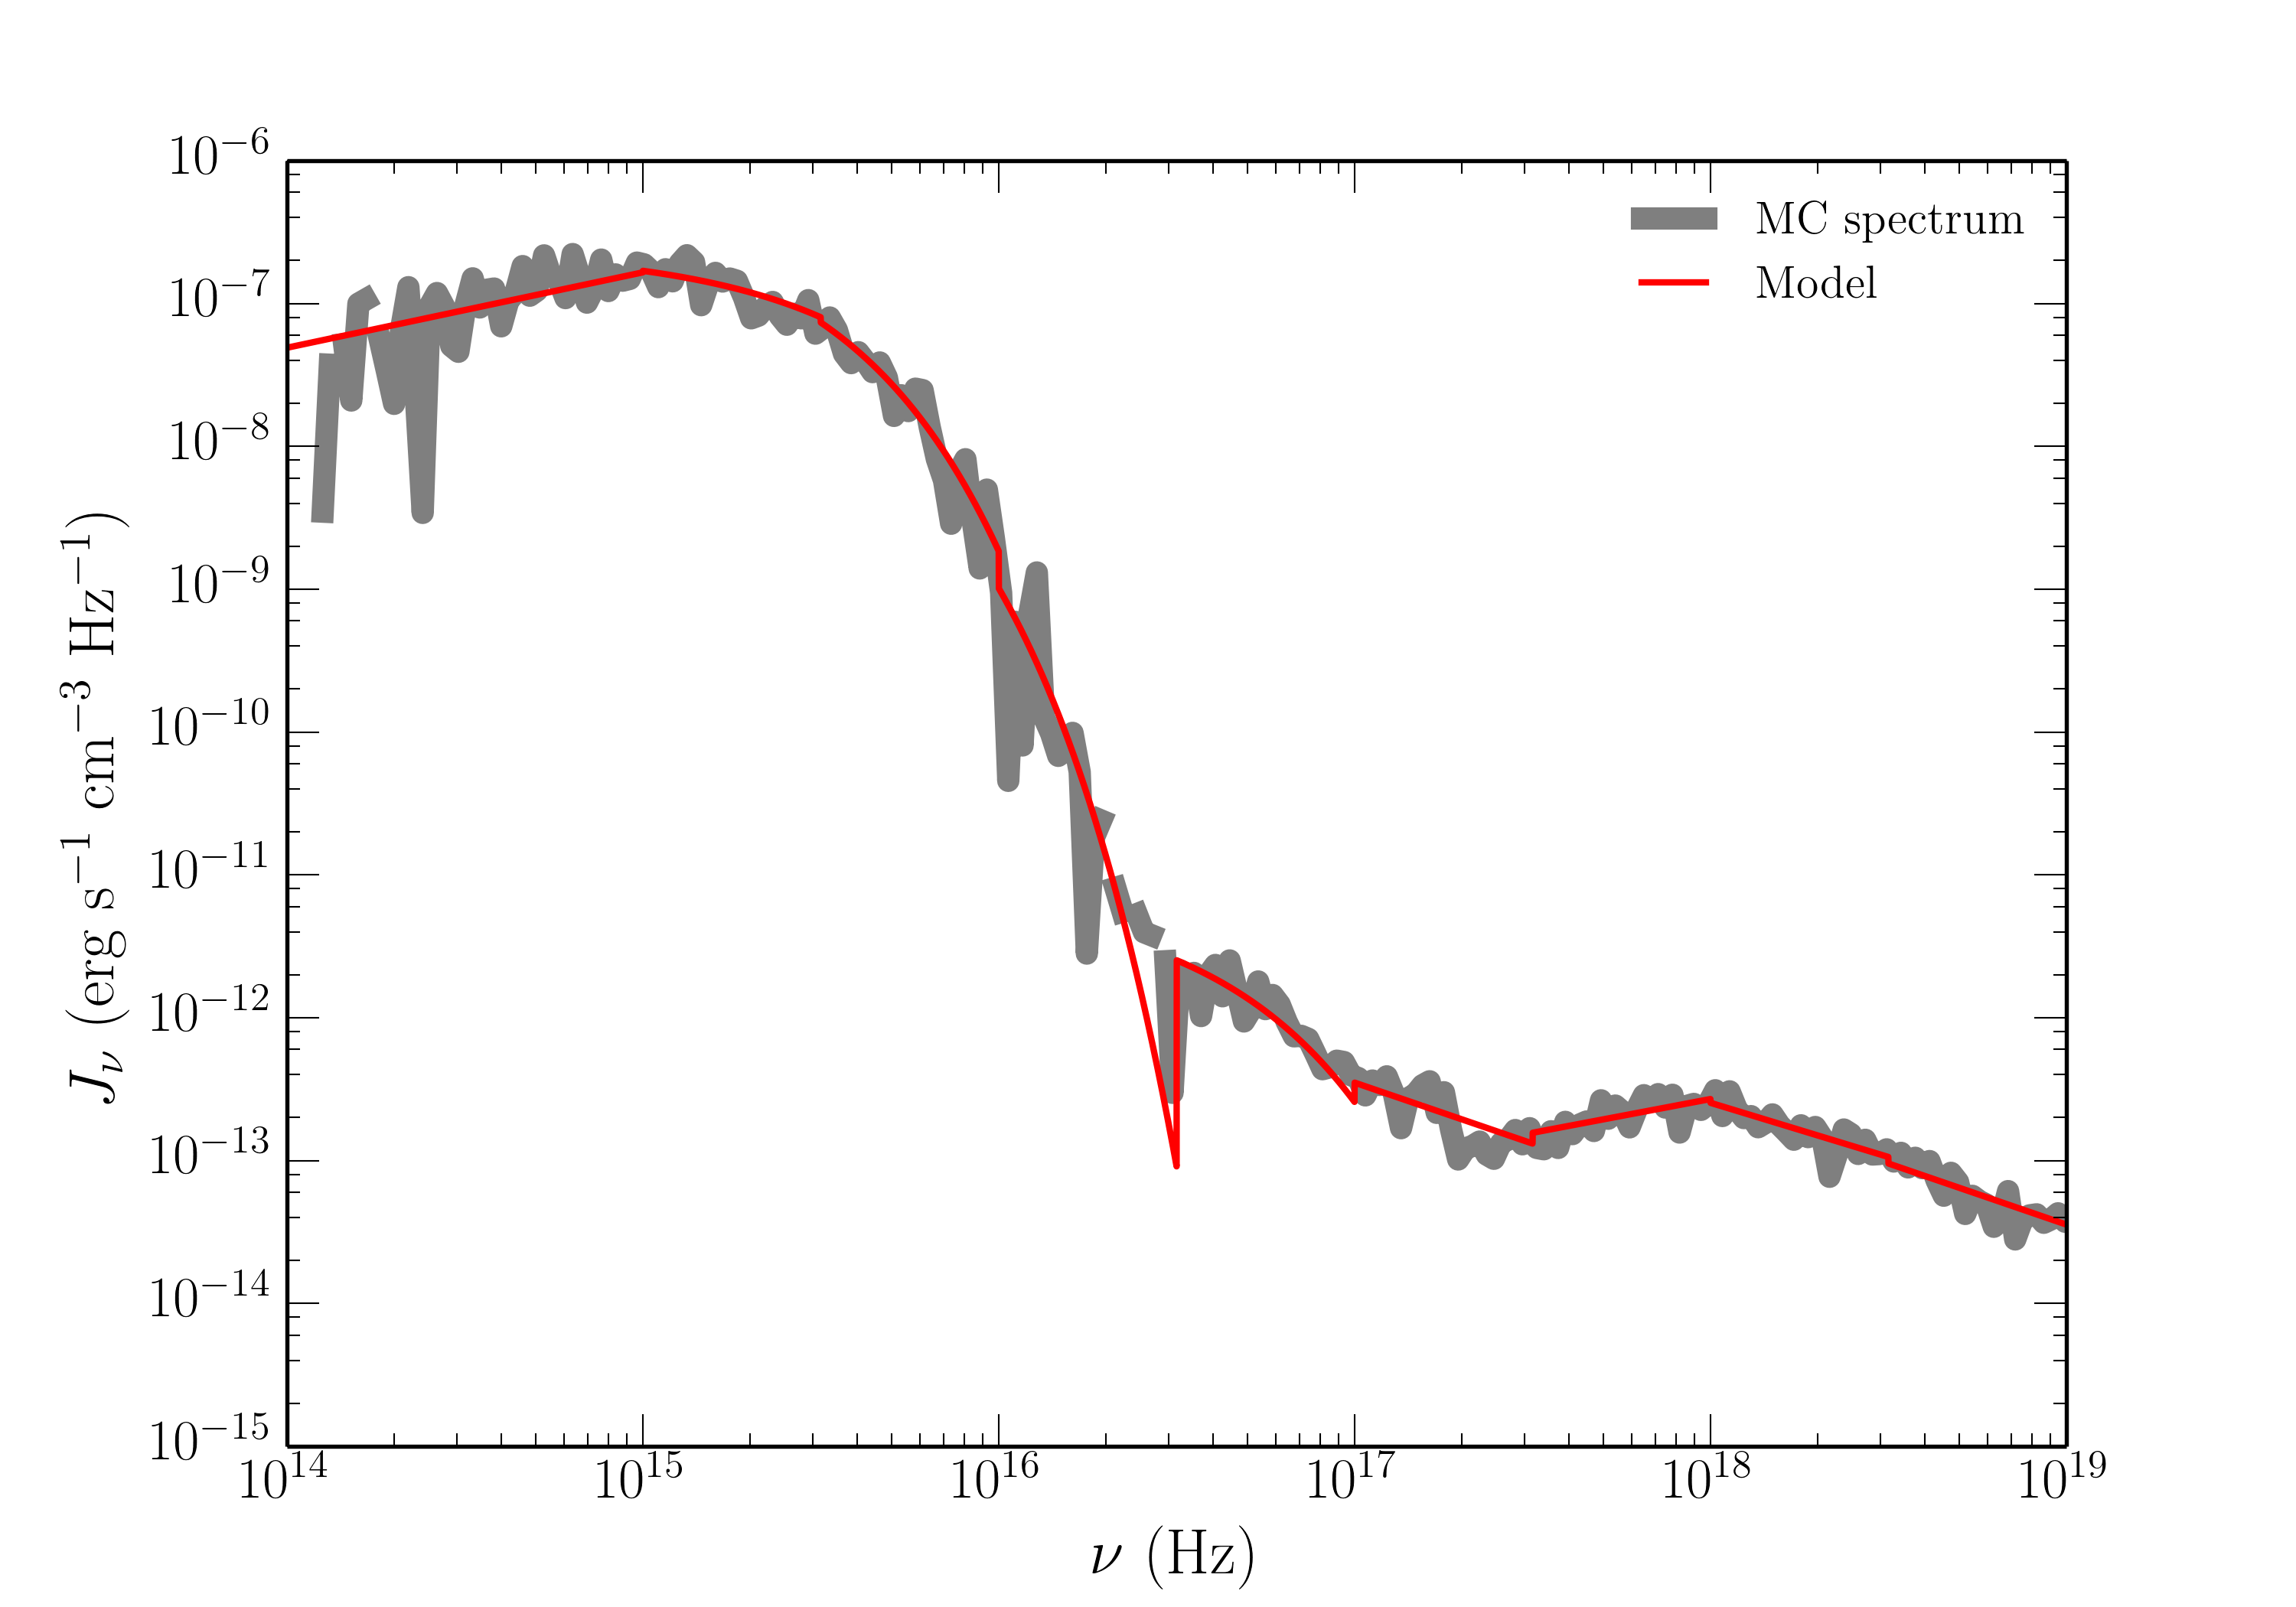
\includegraphics[width=1.0\textwidth]{figures/03-radtrans/cell_spec.png}
\caption
{
An example of a modeled spectrum in \py\ compared to the recorded MC spectrum,
from an individual cell in an AGN model.
} 
\label{fig:cell_spec}
\end{figure}

Once the model for the mean intensity has been calculated, it is possible
to formulate a photoionization rate estimator from ion $i$ to $i+1$ 
for simple-atoms,
\begin{equation}
\gamma_{i,i+1}^S = \sum_i^{\mathrm{bands}} \int_{\nu_i}^{\nu_{i+1}} 
\sum_j^{\mathrm{levels}} \frac{J_{\nu,i} \sigma_{j\kappa}(\nu) }{h \nu} d\nu.
\end{equation}
Recombination rate coefficients are then obtained from 
either tabulated data (see section~\ref{sec:atomic_data})
or, failing that, the Milne relation (equation~\ref{eq:alpha_sp}).

The rate matrix used to calculated the ionization state of simple-atoms
can now be populated. An example rate matrix for H and He would be
\begin{equation}
\begin{bmatrix}
    1  & 1 & 0 & 0 & 0 \\
    \gamma_{H\textsc{i},H\textsc{ii}}^S & -n_e \alpha_{H\textsc{ii},H\textsc{i}} & 0 & 0 & 0 \\
     0 & 0 & 1 & 1 & 1 \\
     0 & 0 & \gamma_{He\textsc{i},He\textsc{ii}}^S & -n_e \alpha_{He\textsc{ii},He\textsc{i}} - \gamma_{He\textsc{ii},He\textsc{iii}}^S & 0\\
     0 & 0 & 0 & \gamma_{He\textsc{ii},He\textsc{iii}}^S & -n_e \alpha_{He\textsc{iii},He\textsc{ii}}
\end{bmatrix}
\begin{bmatrix}
    N_{H\textsc{i}} \\
    N_{H\textsc{ii}} \\
    N_{He\textsc{i}} \\
    N_{He\textsc{ii}} \\
    N_{He\textsc{iii}} 
\end{bmatrix}
=
\begin{bmatrix}
    n_H \\
    0 \\
    n_{He} \\  
    0 \\
    0
\end{bmatrix}
.
\end{equation}
Thus the problem is very similar to solving for level populations in macro-atoms, except that
it is bounded differently.

% Prior to SDL05, the relative ionization fractions for all atomic
% species were estimated via the modified Saha equation (Mazzali \&
% Lucy 1993)  
% \begin{equation}
% \frac{n_{j+1} n_e}{n_j} = W [\xi + W(1-\xi)]
% \left(\frac{T_e}{T_R}\right)^{1/2}
% \left(\frac{n_{j+1}n_e}{n_j}\right)^*_{T_R}. \label{ionization}
% \end{equation}
% Here, the `starred' term on the right represents abundances computed with
% the Saha equation at temperature $T_R$, but using partition functions
% from the dilute blackbody approximation. 
% $W$ is an effective dilution factor, $\xi$ is the
% fraction of recombinations going directly to the ground state, and
% $T_R$ and $T_e$ are the radiation and electron temperatures,
% respectively. This simple ionization scheme produces reasonable
% results when the photoionizing SED can be approximated by a dilute
% blackbody. This is the case for high-state CVs. (As noted above, an
% improved, but more complex treatment of ionization that is appropriate
% for more complex SEDs is described in H13.) 

The rate matrix method with a banded spectral model for the mean intensity is used
in chapter 5 of this thesis, whereas for chapter 4 the dilute approximation is adopted
and ion fractions are obtained from a modified Saha equation (equation~\ref{eq:ml93}).
Regardless of the ionization mode used, the relative excitation fractions of simple-atoms
within each ionization stage of a given species are 
estimated via a modified (dilute) Boltzmann
equation (equation~\ref{eq:dilute_boltzmann}). This equation is approximate, and, in 
general, this approximation is not good. We therefore endeavour to treat any species in
which the excitation state of the ions is thought to be important
in determining either the ionizing radiation field, or emergent spectrum,
as macro-atoms.

% Finally, \py\ originally modelled all bound-bound processes as transitions
% within a simple two-level atom \cite[e.g.][]{mihalas}. 
% This framework was used for the treatment of line transfer and also
% for the line heating and cooling calculations (see LK02). 
% The approximation works reasonably well for resonance  
% lines, such as \civfull, in which the lower level is the ground state.  
% However, it is a poor approximation for many other
% transitions, particularly those where the upper level
% is primarily populated from above. Thus an improved method for
% estimating excited level populations and simulating line transfer is
% needed in order to model recombination lines and continua.

\section{Heating And Cooling Balance}
\label{sec:heating_cooling}
I have already given the estimators used to calculate
heating and cooling rates in the plasma. These are not only used
in the creation and elimination of $k$-packets, but also in the heating
and cooling balance carried out in \py\ to achieve a self-consistent
temperature structure in the wind. 

At the end of each ionization cycle, the code has stored a new set
of MC estimators for radiative heating of the plasma. We then
assume that each cell is in thermal equilibrium, so that the appropriate
electron temperature is simply the value of $T_e$ that is a solution
to the equation
\begin{equation}
\hh_{\mathrm{tot}} - \cc_{\mathrm{tot}} ( T_e) = 0,
\end{equation}
where $\hh_{\mathrm{tot}}$ and $\cc_{\mathrm{tot}}$ are the total heating and cooling rates in 
the plasma. A number of checks are in place to ensure numerical stability,
namely a maximum temperature and a maximum change in temperature from cycle
to cycle. This is especially important in cases where the initial
guess at the wind temperature is far from the true value.

\subsection{Convergence}

\label{sec:convergence}

\py\ always runs a fixed number of ionization cycles, rather than terminating
when a convergence criterion is reached. As a result, it is up to the user
to check that the simulation is converged. An individual cell is considered
converged when a) the temperature stops changing signicantly, i.e. both
$T_R$ and $T_e$ satisfy
\begin{equation}
\frac{|T_{\mathrm{new}} - T_{\mathrm{old}}|}{T_{\mathrm{new}} + T_{\mathrm{old}}} < 0.05,
\end{equation}
and b) the heating and cooling rates are well balanced, such that
\begin{equation}
\frac{|\hh_{\mathrm{tot}} - \cc_{\mathrm{tot}}|}{\hh_{\mathrm{tot}} + \cc_{\mathrm{tot}}} < 0.05.
\end{equation}
These criteria could doubtless be improved, but they are nonetheless
a good way of ensuring that thermal and radiative equilibrium holds in the 
plasma. An example of how the average temperature and fraction
of converged cells changes over the course of the ionization cycles in
a typical CV model is shown in Fig.~\ref{fig:conv}.


\begin{figure}
\centering
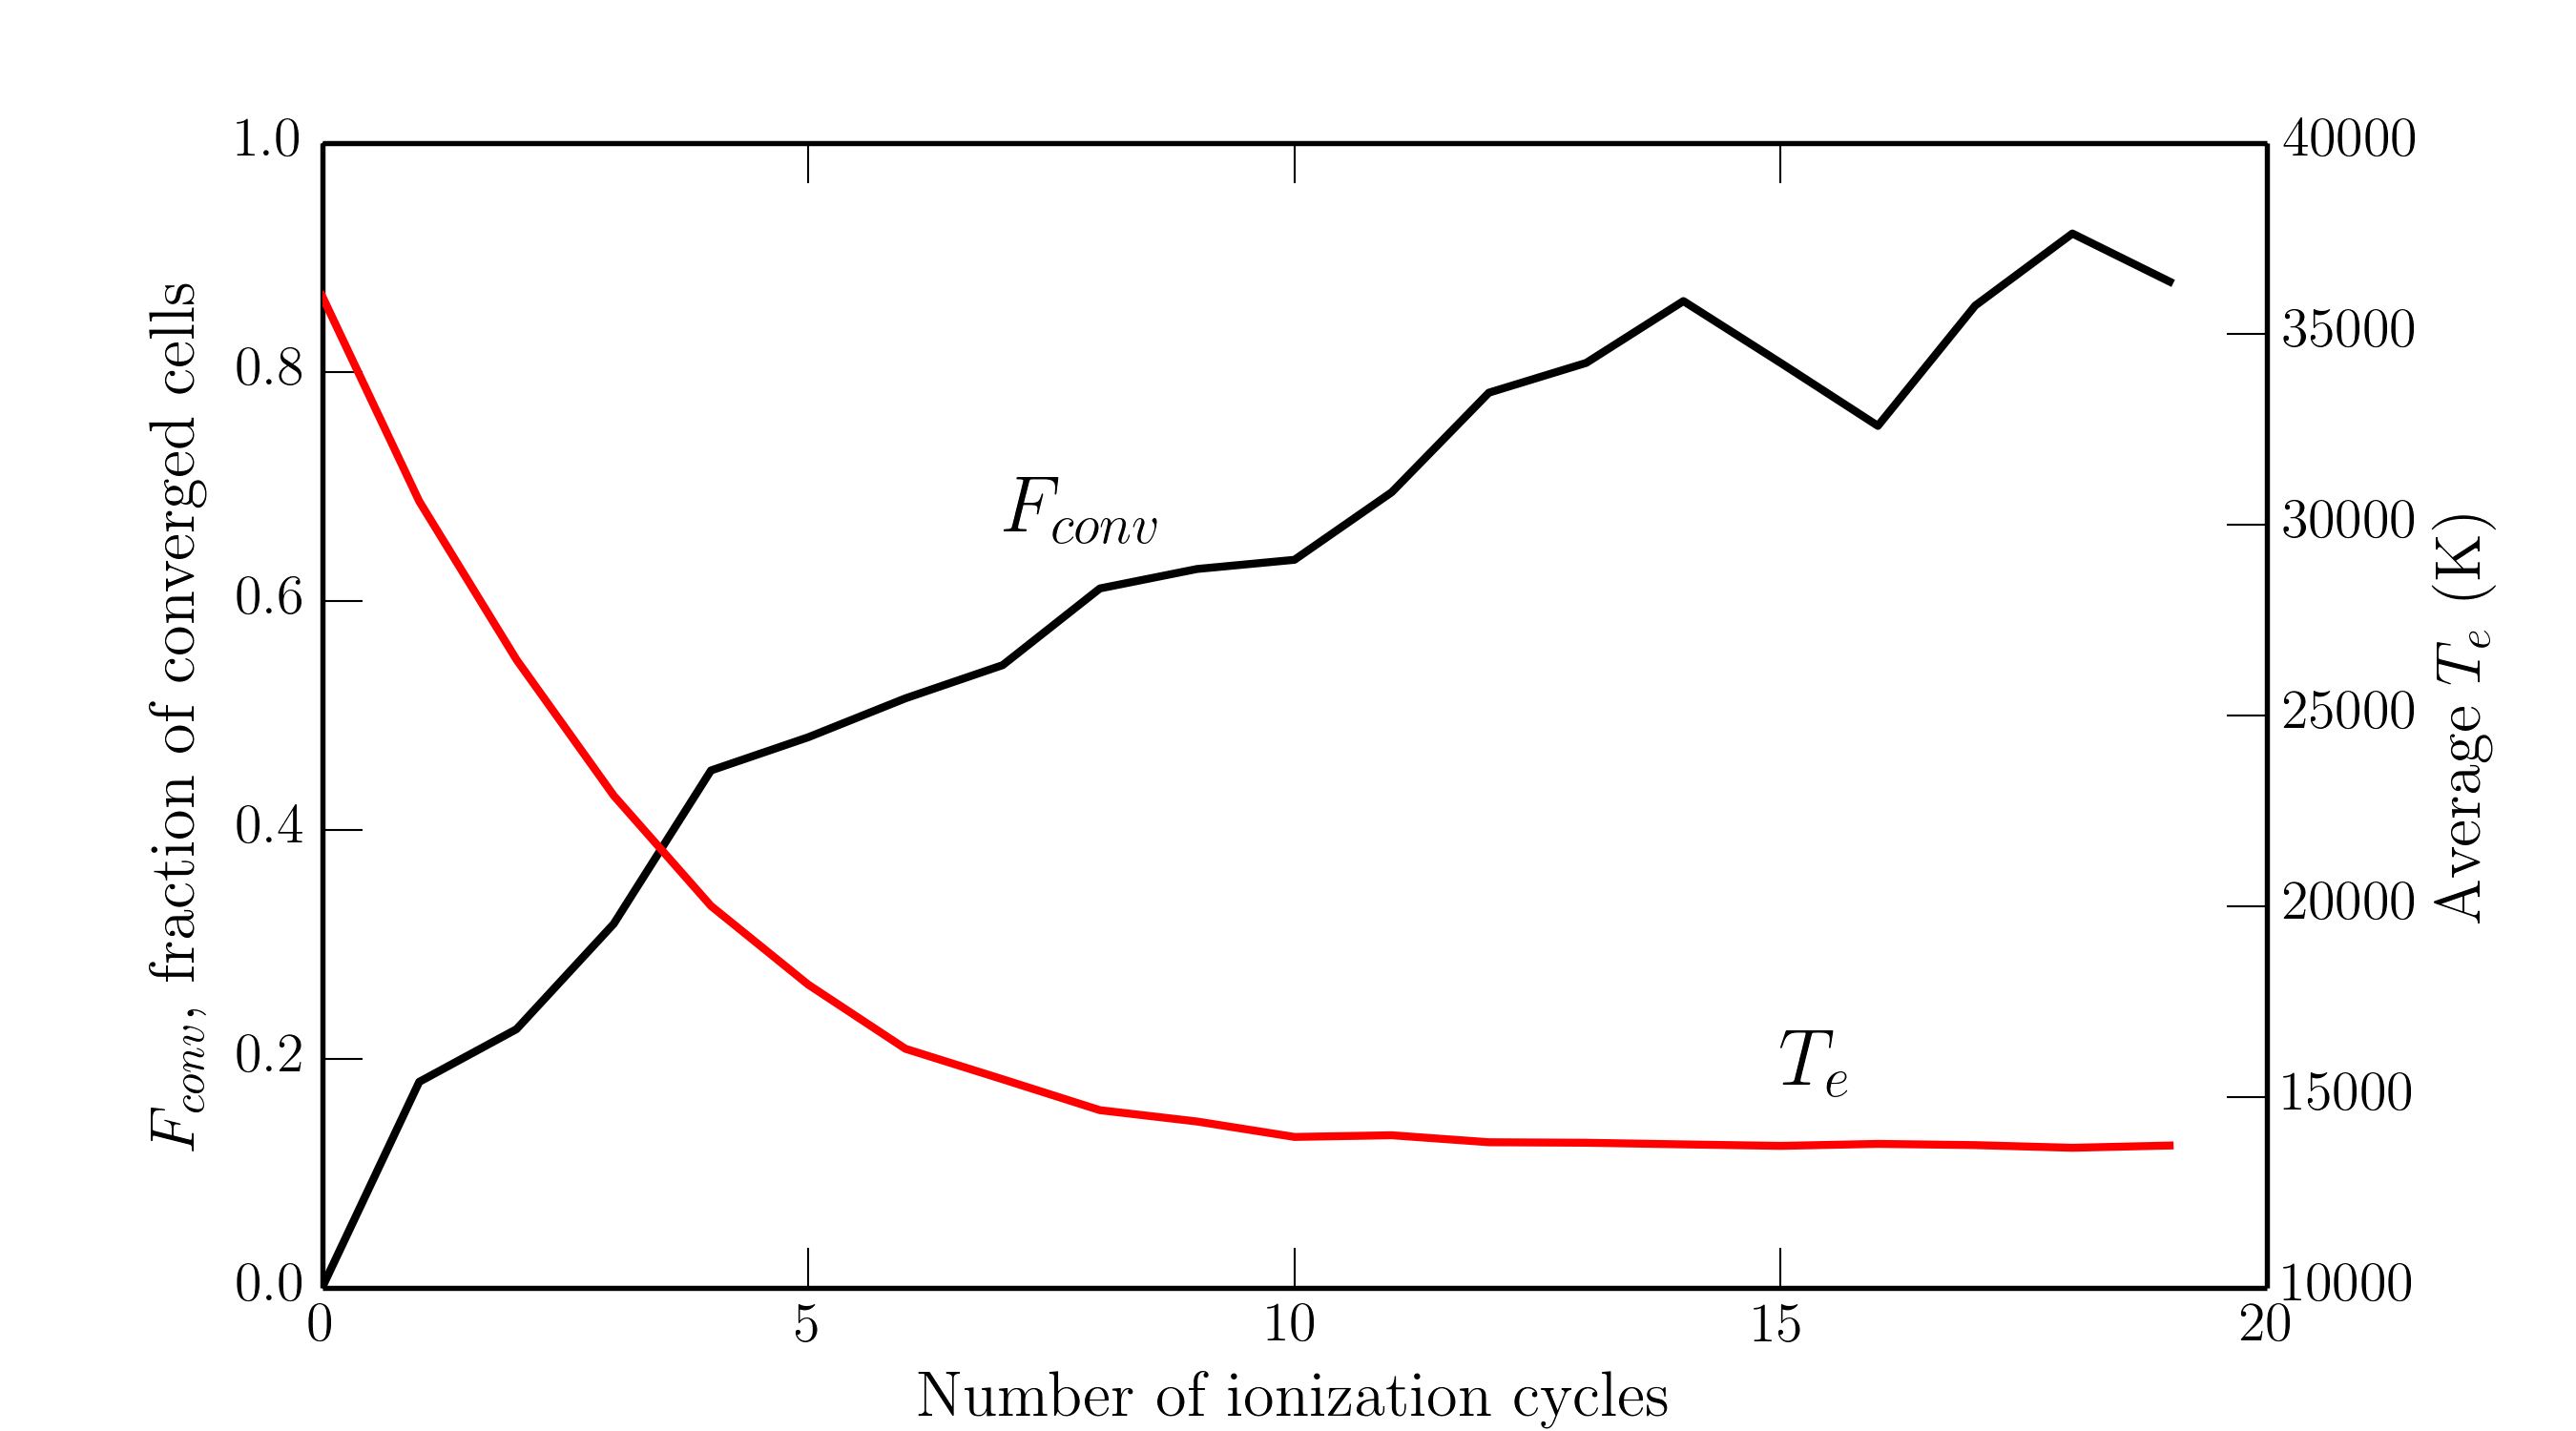
\includegraphics[width=1.0\textwidth]{figures/03-radtrans/graph_conv.png}
\caption
{
The average temperature and fraction of converged cells in
a typical CV model, shown as a function of the number of ionization cycles
completed. 
} 
\label{fig:conv}
\end{figure}




\section{Spectral Cycles}
\label{sec:spectral_cycles}
The primary output from \py\ is a synthetic spectrum over a specific wavelength
range produced at user-specified viewing angles. This spectrum is produced 
in a separate cycle from the calculation of the ionization state, as we are then concerned
with producing detailed, high-resolution spectra in a specific wavelength regime
that can then be compared to observations.

The code utilises a variance reduction technique in order to minimise the amount of 
time spent in this portion of the code. This technique is based 
on a similar method implemented by \cite{woods1991} and is known in the code
as the `extract' method. This method works by 
tracking photon packets until they scatter or interact with the plasma, according
to the procedure described in section~\ref{sec:rt_procedure}. 
At the scattering location, the optical depth the photon would
experience were it to escape to infinity along each requested viewing angle, 
$\tau_{\mathrm{extract}}(\theta_i)$, is calculated. The spectrum at each 
viewing angle $\theta_i$ is then incremented by an amount
\begin{equation}
\Delta L = w f(\theta_i) \exp(-\tau_{\mathrm{extract}}(\theta_i)),
\end{equation}
where $w$ is the weight of the photon, and $f(\theta_i)$ is a weighting proportional to
the probability that the photon would have scattered in direction $\theta_i$. Once this
value has been added to the corresponding wavelength bin, the photon
proceeds as normal in its new random direction.

In the alternative `live or die' method this extraction procedure is not
carried out, and a user simply has to run a sufficient number of 
photons to ensure that enough will happen
to fall into the finite solid angle bins requested. This is significantly
less efficient. A comparison between the two methods is shown in 
figure~\ref{fig:extract_demo} for a standard CV model, showing that the spectrum 
produced is identical in shape, but with significantly higher signal-to-noise (for
fixed number of cycles) in the `extract' case.

\begin{figure}
\centering
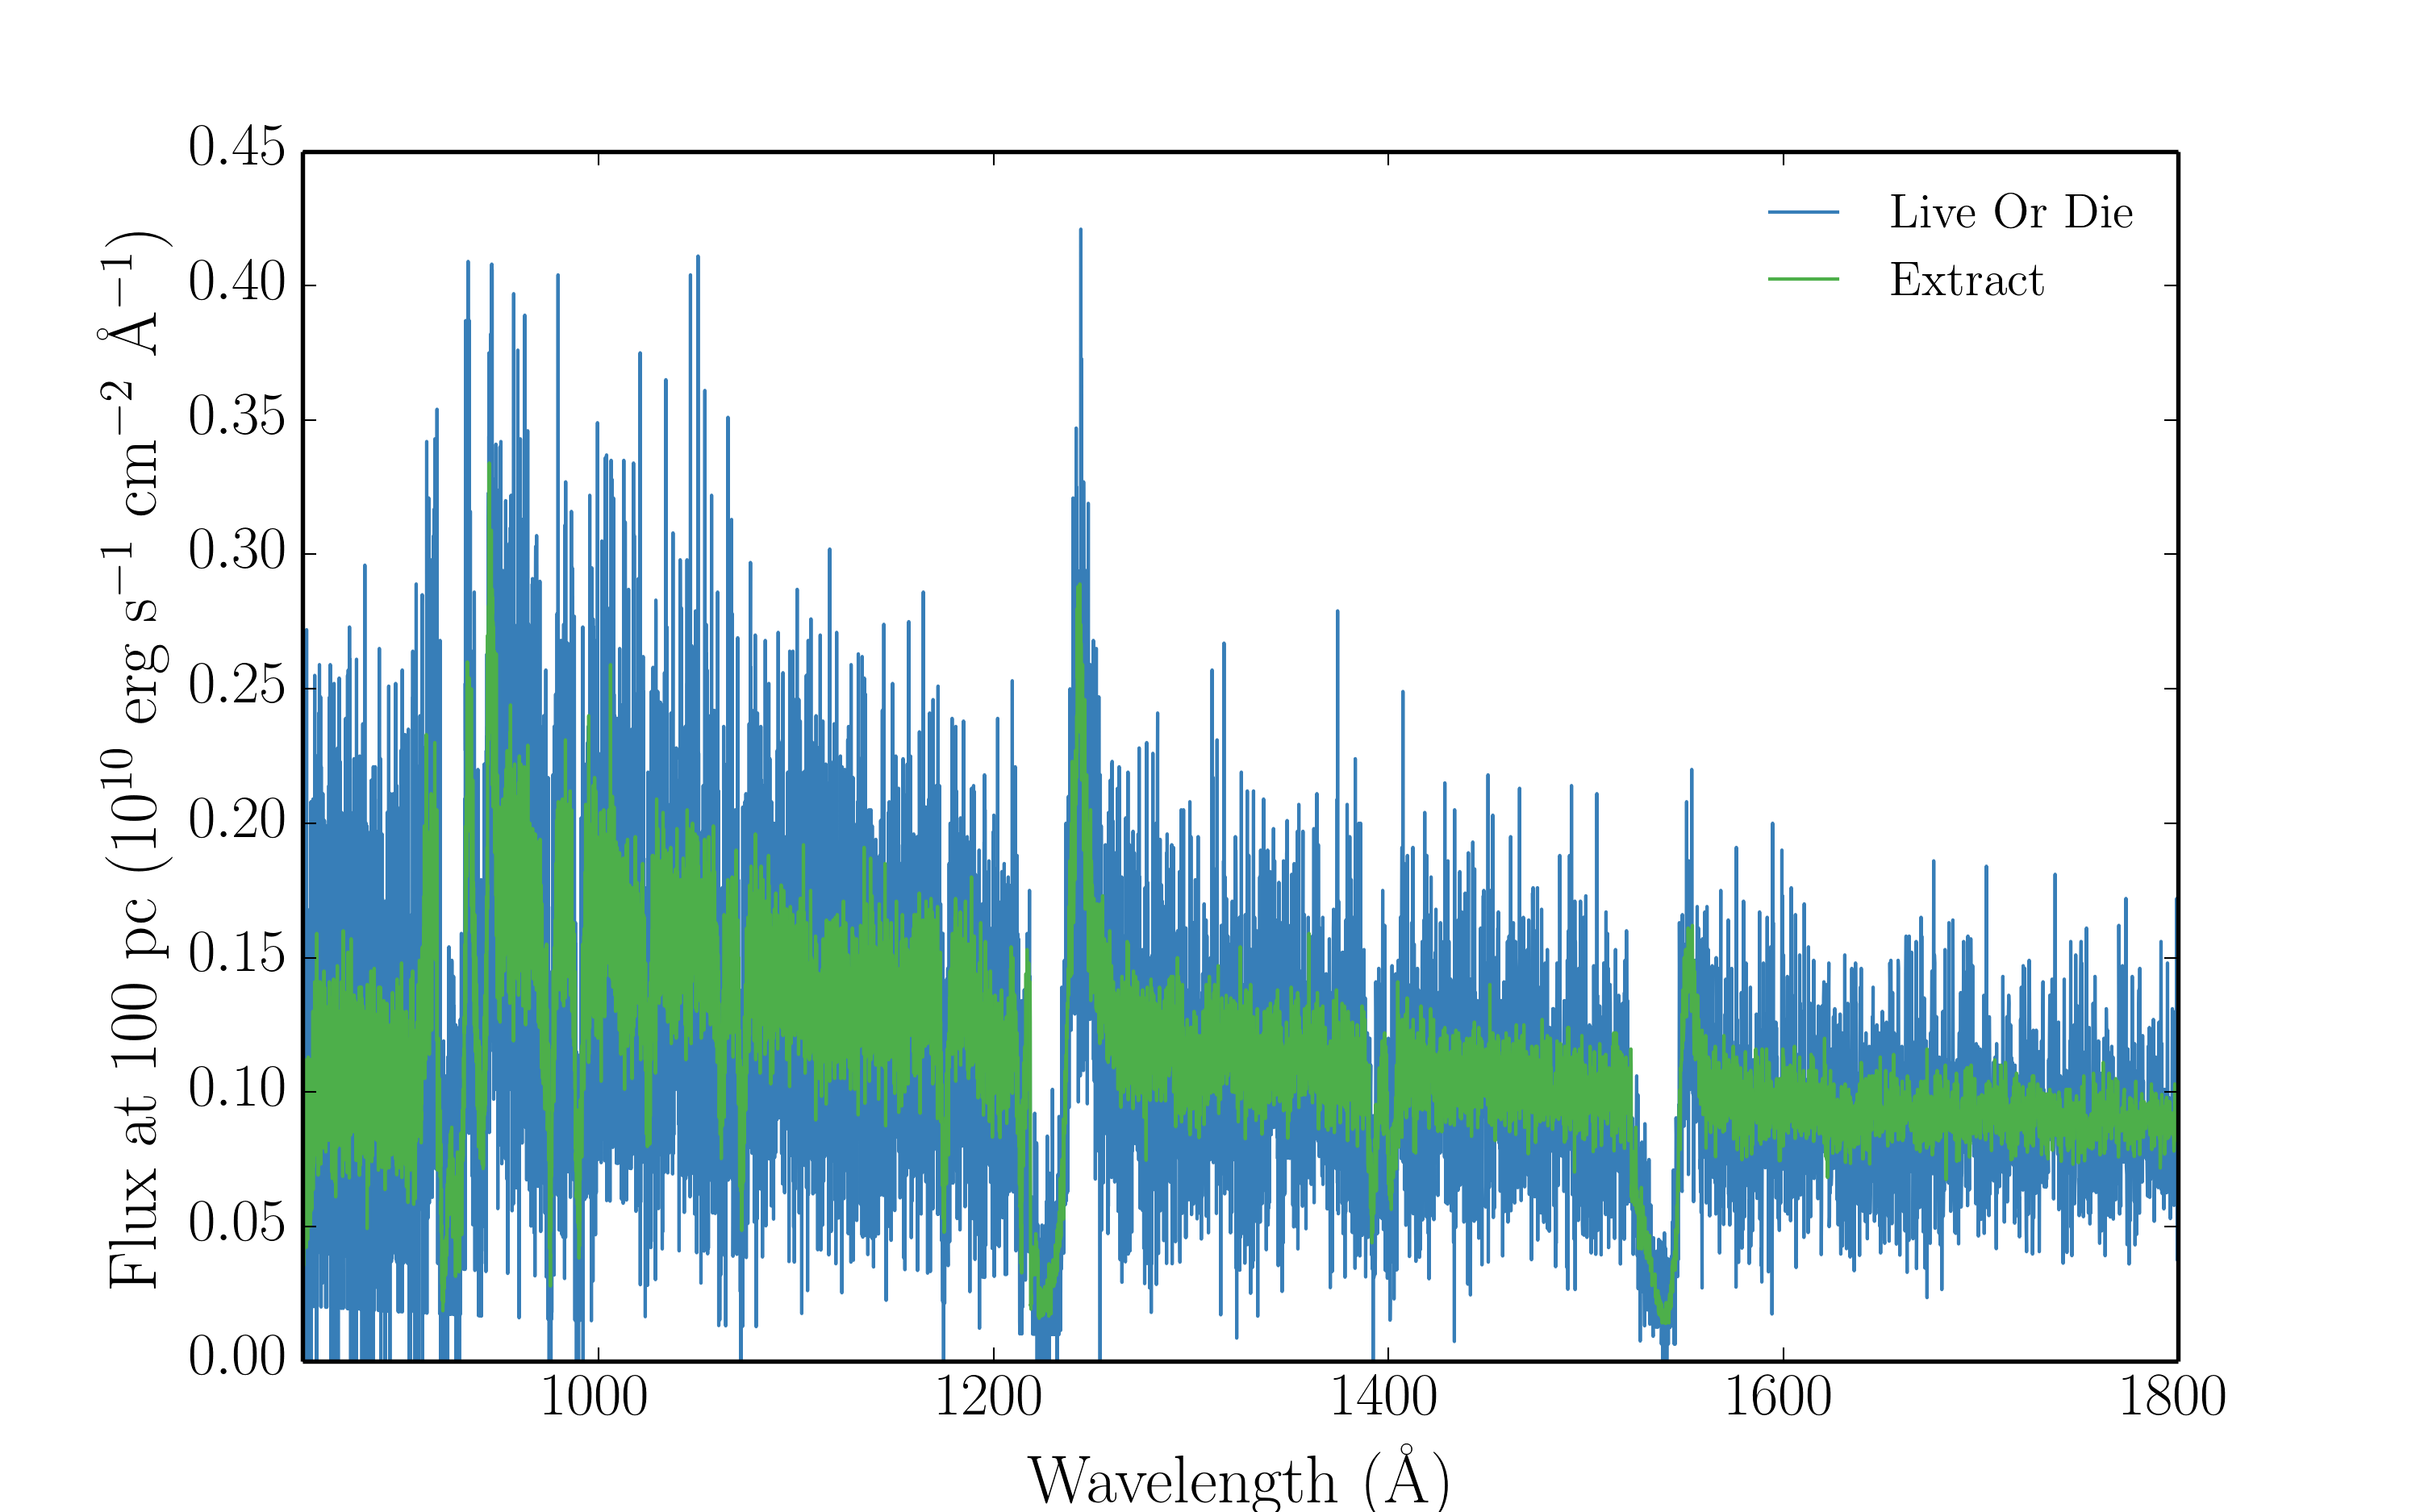
\includegraphics[width=1.0\textwidth]{figures/03-radtrans/extract_demo.png}
\caption
[A comparison of synthetic spectra produced in extract and live or die modes.]
{
A synthetic spectrum after $30$ spectral cycles with $100,000$ photons
from simple CV wind model at a $60^\circ$ viewing angle.
Spectra produced with both the extract and live or die modes
are shown. The effectiveness of the extract variance reduction technique can
be clearly seen, and we can see that the spectral shape is unaltered.
} 
\label{fig:extract_demo}
\end{figure}

\subsection{Macro-atom Emissivity Calculation}

In order to preserve the philosophy that a detailed 
spectrum is calculated in a limited wavelength regime, \py\ carries
out a macro-atom emissivity calculation before the spectral cycles.
The aim of this step is to calculate the luminosity contributed
by macro-atoms -- equivalent to the total amount of reprocessed emission -- 
in the wavelength range being considered.

This process can be very computationally intensive, especially if the wavelength regime
being simulated has very little emission from bound-free and line processes
in the wind, but the overall broad-band emissivity is high.
During the ionization cycles, the amount of energy absorbed into $k$-packets and 
every macro-atom level is recorded using MC estimators. Once 
the ionization cycles are finished, and the model has converged, these absorption
energies are split into a certain number of packets and tracked through
the macro-atom machinery until a deactivation occurs. When this happens,
the emissivity of the level the macro-atom de-activated from is incremented
if the packet lies in the requested wavelength range. If it does not, then 
the packet is thrown away. It is easy to see how what is essentially a MC rejection
method can be an inefficient way of sampling this parameter space. Fortunately,
this problem is parallelisable (see section~\ref{sec:parallel}).

Once the emissivities have been calculated, the spectral synthesis can proceed.
This is done in a different way to the ionization cycles. Photons 
are generated from the specified photon sources over the required wavelength range,
but are now also generated according to the calculated macro-atom and 
$k$-packet emissivities in each cell. These photons are `extracted' according
to the procedure outlined above.
In order to ensure that radiative equilibrium 
still holds, any photon that interacts with a macro-atom or $k$-packet is immediately 
destroyed. The photons are tracked and extracted as normal until they escape the 
simulation; resonant scatters are dealt with by a combination of
macro-atom photon production and destruction.

\section{Atomic Data}
\label{sec:atomic_data}
One of the big challenges in building reliable photoionization and radiative
transfer codes lies in the acquisition of accurate and complete atomic datasets.
All of the rates described so far contain a term, such as the oscillator strength 
or dimensionless collision strength, that is dependent purely on the atomic physics
associated with the transition. These quantities can be measured in laboratory experiments,
or predicted from atomic structure codes that derive the atomic physics from 
quantum theory.

Throughout this work, I have used very similar atomic data to that described 
by LK02 and H13. Elements included are H, He, C, N, O, Ne, Na, Mg, Al, Si, S,
Ar, Ca and Fe, although this can be easily be adapted. Solar abundances from
\cite{vernerbarthel1994} are adopted, and ionization potentials and ion
multiplicities are from \cite{verner1996}. Line information for simple-atoms 
is obtained from \citet[][$\sim5,000$ lines]{verner1996} 
and \citet[][$\sim55,000$ lines]{kurucz1995}. 
The level information for simple-atoms is constructed 
from the line lists using the technique described by \cite{lucy1999sne}.

Radiative recombination rate coefficients are taken from 
the \textsc{Chianti} database version 7.0 \citep{dere1997,landi2012}.
Ground state recombination rates from \cite{badnell2006} are adopted where available,
otherwise the code defaults to calculating recombination rates from the Milne
relation. Free-free Gaunt factors are from \cite{sutherland1998}.

\subsection{Macro-atom Level and Line Data}

A 20-level model H atom was incorporated into \py\ by SDL05,
and includes line oscillator strengths from \cite{menzel1935}.
This model atom is only split according to principle quantum number $n$,
and it is thus assumed that collisions in the plasma will cause 
the $l$-subshells to be populated according to statistical weights. 
This is known as {\em $l$-mixing} and is a good approximation for hydrogen in
dense astrophysical plasmas due to the near degeneracy of the subshell 
energy levels.

In order to correctly model He recombination lines in CVs and AGN, such as the 
prominent \heiiuv\ line, I have expanded the atomic data set, so that \py\
now contains all the atomic data needed for a He macro-atom. This data was 
obtained from \textsc{Topbase}, except for some inaccurate line wavelengths
that were set to the experimental values from the National 
Institute of Standards and Technology (NIST\footnote{\url{http://www.nist.gov/}}).
He~\textsc{i} is split into $l$ and $s$ subshells so as to correctly model the
singlet and triplet lines observed in many optical spectra. He~\textsc{ii} is assumed
to be $l$-mixed, as it is hydrogenic.

For CV modelling (chapter 4), I used the full 20-level hydrogen atom, with 53 levels of 
He~\textsc{i} up to principle quantum number 10, and 10 levels of He~\textsc{ii}. 
Modelling levels close to the continuum energy can
provide a performance hit in macro-atom mode, but is necessary
when modelling recombination lines from excited 
upper levels. In quasar models (chapter 5) 
this is not as important, and the
plasma is generally more ionized. There, a 10-level hydrogen atom was used and
He~\textsc{i} was treated with only the ground state -- this simplification
had no effect on the temperature structure of the wind or emergent spectrum.

\subsection{Photoionization Cross-sections}

Photoionization cross-sections are from \textsc{Topbase} \citep{cunto1993} and from 
\cite{vfky}.
Where possible, I use \top\ photoionization cross-sections. For macro-atoms,
these cross-sections are partial and represent the cross-section for a photoionization
from a given {\em level}. We neglect photoionizations to excited configurations
of the upper ion. For simple-atoms they are from the ground state.
The \top\ cross-sections have two major drawbacks in that they do not 
extend to particularly high energies and do not always contain accurate threshold
energies.

In order to improve the \top\ cross-sections, I extrapolated them to larger
energies. This was done by finding the slope, in log-log space,
of the cross-section at the maximum energy, and extrapolating to $100$~keV.
In some cases, the slope near the maximum energy was anomalous 
due to resonances or similar structure in the cross-section, or possibly
simply due to unknown problems in the \top\ calculations. These
cases were identified by eye and a $\nu^{-3}$ extrapolation
was then applied instead. 
The results of this extrapolation on the soft X-rays in an AGN model
are shown in figure~\ref{fig:xs}. Where previously there was a sharp,
unphysical edge due to the lack of high energy 
($\nu \gtrsim 10^{18}~\mathrm{Hz}$) data, 
there is now a smooth recovery to an X-ray 
power law we expect. I also manually adjusted the threshold energies in some
cases to match the more accurate values from \cite{vfky}.

\begin{figure}
\centering
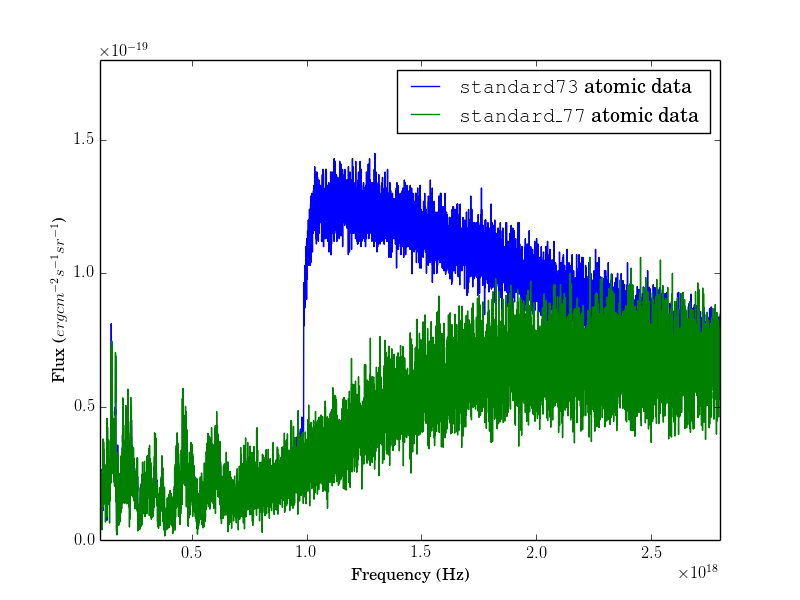
\includegraphics[width=1.0\textwidth]{figures/03-radtrans/xs.png}
\caption
[The effect of extrapolated cross-sections on the soft X-ray spectrum]
{
A comparison of the soft X-ray regime of the H13 model, with two different
datasets. standard73 is the dataset with old, unextrapolated cross-sections 
and standard77 instead includes extrapolated cross-sections as described in
the text.
}
\label{fig:xs}
\end{figure}

% \section{Clumping}

% \label{sec:microclumping}

% \subsection{Motivation}

% As described in section~??, observational evidence for inhomogeneities in 
% outflows is widespread. Clumping a plasma can have a significant effect on its
% ionization, emission and absorption characteristics. Clearly, the interplay between
% these effects will be somewhat complex 

% A number of different implementations of clumping have been explored in previous studies,
% mostly in the stellar winds community. Perhaps the simplest method is 
% when one assumes that the individual clumps are both optically and geometrically thin;
% this is known as {\em microclumping} \citep[e.g.][]{hamann1998,hilliermiller1999,hamann2008}. 
% This technique has been particularly successful in reconciling 
% discrepant mass-loss estimates.
% It was found that one would obtain different mass-loss rates depending on whether
% they were calculated from (i) UV resonance scattering of continuum photons 
% (which scales linearly with density; a `$\rho$-diagnostic') or (ii) recombination 
% and free-free emission process (which scale with the square of density; 
% `$\rho^2$-diagnostics'). A clumped outflow would have enhanced densities in 
% certain regions, and would thus mean that $\rho^2$-diagnostics tend to 
% overestimate the total mass-loss rates. Microclumping has helped verify this
% hypothesis with radiative transfer modelling (REFs). These clumpy models also
% provide better fits to the electron scattering wings of emission lines in stellar
% winds \citep{hillier1991}.

% The second-generation of stellar wind codes went on step further by addressing the issue
% of {\em porosity}; that clumps will have a finite size, and thus gaps between the clumps
% may affect the emergent radiation field. This approach is known as {\em macroclumping}.
% {\bf Describe macroclumping with references.}

% Implementing a treatment of clumping in accretion disc wind models is challenging, for
% two main reasons. First, the physical scale lengths and density contrasts 
% in disc winds are not well-constrained from observations, especially in AGN.  
% Second, there are significant computational difficulties associated with adequately
% resolving and realistically modelling a series of small scale, high density
% regions with a MCRT code. Given the lack of knowledge about the actual 
% type of clumping, we encorporated the simpler microclumping approach into our code.
% This is partly because our primary concern was the ionization and 
% emission characteristics of the flow, and porosity was a secondary concern.


% \subsection{Microclumping}

% To take account of clumping in our outflow we adopt a simple parameterization
% used in stellar wind modelling. The key assumption here is that typical clump sizes
% are much smaller than the typical photon mean free path, and thus the clumps are 
% both geometrically and optically thin. This approach is typically 
% known as microclumping and allows one to introduce a `filling factor', $f$, which is the 
% fraction of the volume of the plasma filled by clumps. We can then introduce the 
% `density enhancement', $D$, which is simply 

% \begin{equation}
% D = \frac{1}{f}
% \end{equation}

% The densities in the model are then multiplied by this factor. This has the effect 
% of enhancing `$\rho^2$' processes such as recombination or collisional excitation,
% and 


\section{Code Validation}
\label{sec:code_validation}

The main challenge for high performance scientific computing can be 
elegantly summarised by the \cite{ferland2002} epitaph, {\sl `Reliability in the face 
of complexity'}. I have already delved into some of the complexity in this case,
so it is important to establish whether the code is also reliable before I present
results. 

\subsection{Testing Against \cld}

\cld\ is a spectral synthesis and photoionization code used to simulate
the emergent spectrum and ionization conditions in nebulae and other plasma
environments. As a result, it uses many of the same techniques as \py\
in order to compute ionization states, level populations and heating and cooling
rates. It thus represents an excellent benchmarking tool. \py\ has been tested extensively
against \cld\ in the past; some of these successful
tests can be found in H13 and LK02.

Figs.~\ref{fig:h_cloudy} to \ref{fig:ir_cloudy} show a series of 
ionization plots with relative ion fractions plotted as a function of
ionization parameter, $U$. The ionization parameter is a useful
way to parameterise the ionization state of a plasma, and is given by
\begin{equation}
U = \frac{4\pi}{n_H c}\int_{13.6{\rm{eV}} / h}^{\infty}\frac{{J_{\nu}d\nu}}{h\nu}.
\label{eq:ip}
\end{equation}
In \py, the ionization parameter in a cell
is calculated via a MC estimator, such that
\begin{equation}
U_{\py} = \frac{1}{c~V~n_H} \sum_i^{\mathrm{photons}} \frac{w_i \Delta s}{h \nu}.
\end{equation}
This test is designed to check that \py\ still agrees
well with \cld\ when we turn on the full macro-atom machinery.
The calculations are conducted using the same 
incident SEDs, densities and abundances, and \py\ is operated in
1D, thin shell mode to simulate an optically thin plasma and facilitate
comparison with \cld. I have shown two separate ionization modes
from \py: standard mode, in which nothing is treated as a macro-atom
and the spectral model ionization scheme of H13 is used to calculate
ion fractions, and hybrid mode in which H and He are treated as 
macro-atoms and their level populations and ion fractions are solved
using MC estimators according to the routine
described in section~\ref{sec:matom_pops}. Thus, in both 
cases the simple-atoms have their populations calculated using the H13 scheme.

In general, the calculated fractions are in excellent agreement, with a few 
exceptions. The first problem is with He at low ionization parameters 
(see Fig.~\ref{fig:he_cloudy}), where there is a discrepancy between 
the macro-atom solution and the standard mode solution. This is due to 
differences in the calculated recombination rate. In macro-atom mode, 
this is done using the Milne relation for all the bound-free jumps that 
have been identified, which currently includes all transitions from the lower ion but
ignores transitions to excited states of the upper ion. However, 
in standard mode \py\ uses the recombination rates from Chianti,
which represent a weighted sum over all the possible bound-free transitions,
and are thus in some ways more complete. Neverthless, the macro-atom
scheme is self-consistent, in that all photoionization pathways have a matching 
recombination pathway, and the level populations are calculated much more
accurately. Furthermore, the models presented later generally have 
$\log U \gtrsim -2$, where the calculation
agrees well with \cld\ and standard mode.
The second problem lies in Fe, where there can be quite large differences
between \py\ and \cld. This is mainly due to Auger ionization and charge 
exchange and has recently been improved in \py. 
The effect on quasar models is discussed in chapter 5. 


\begin{figure}
\centering
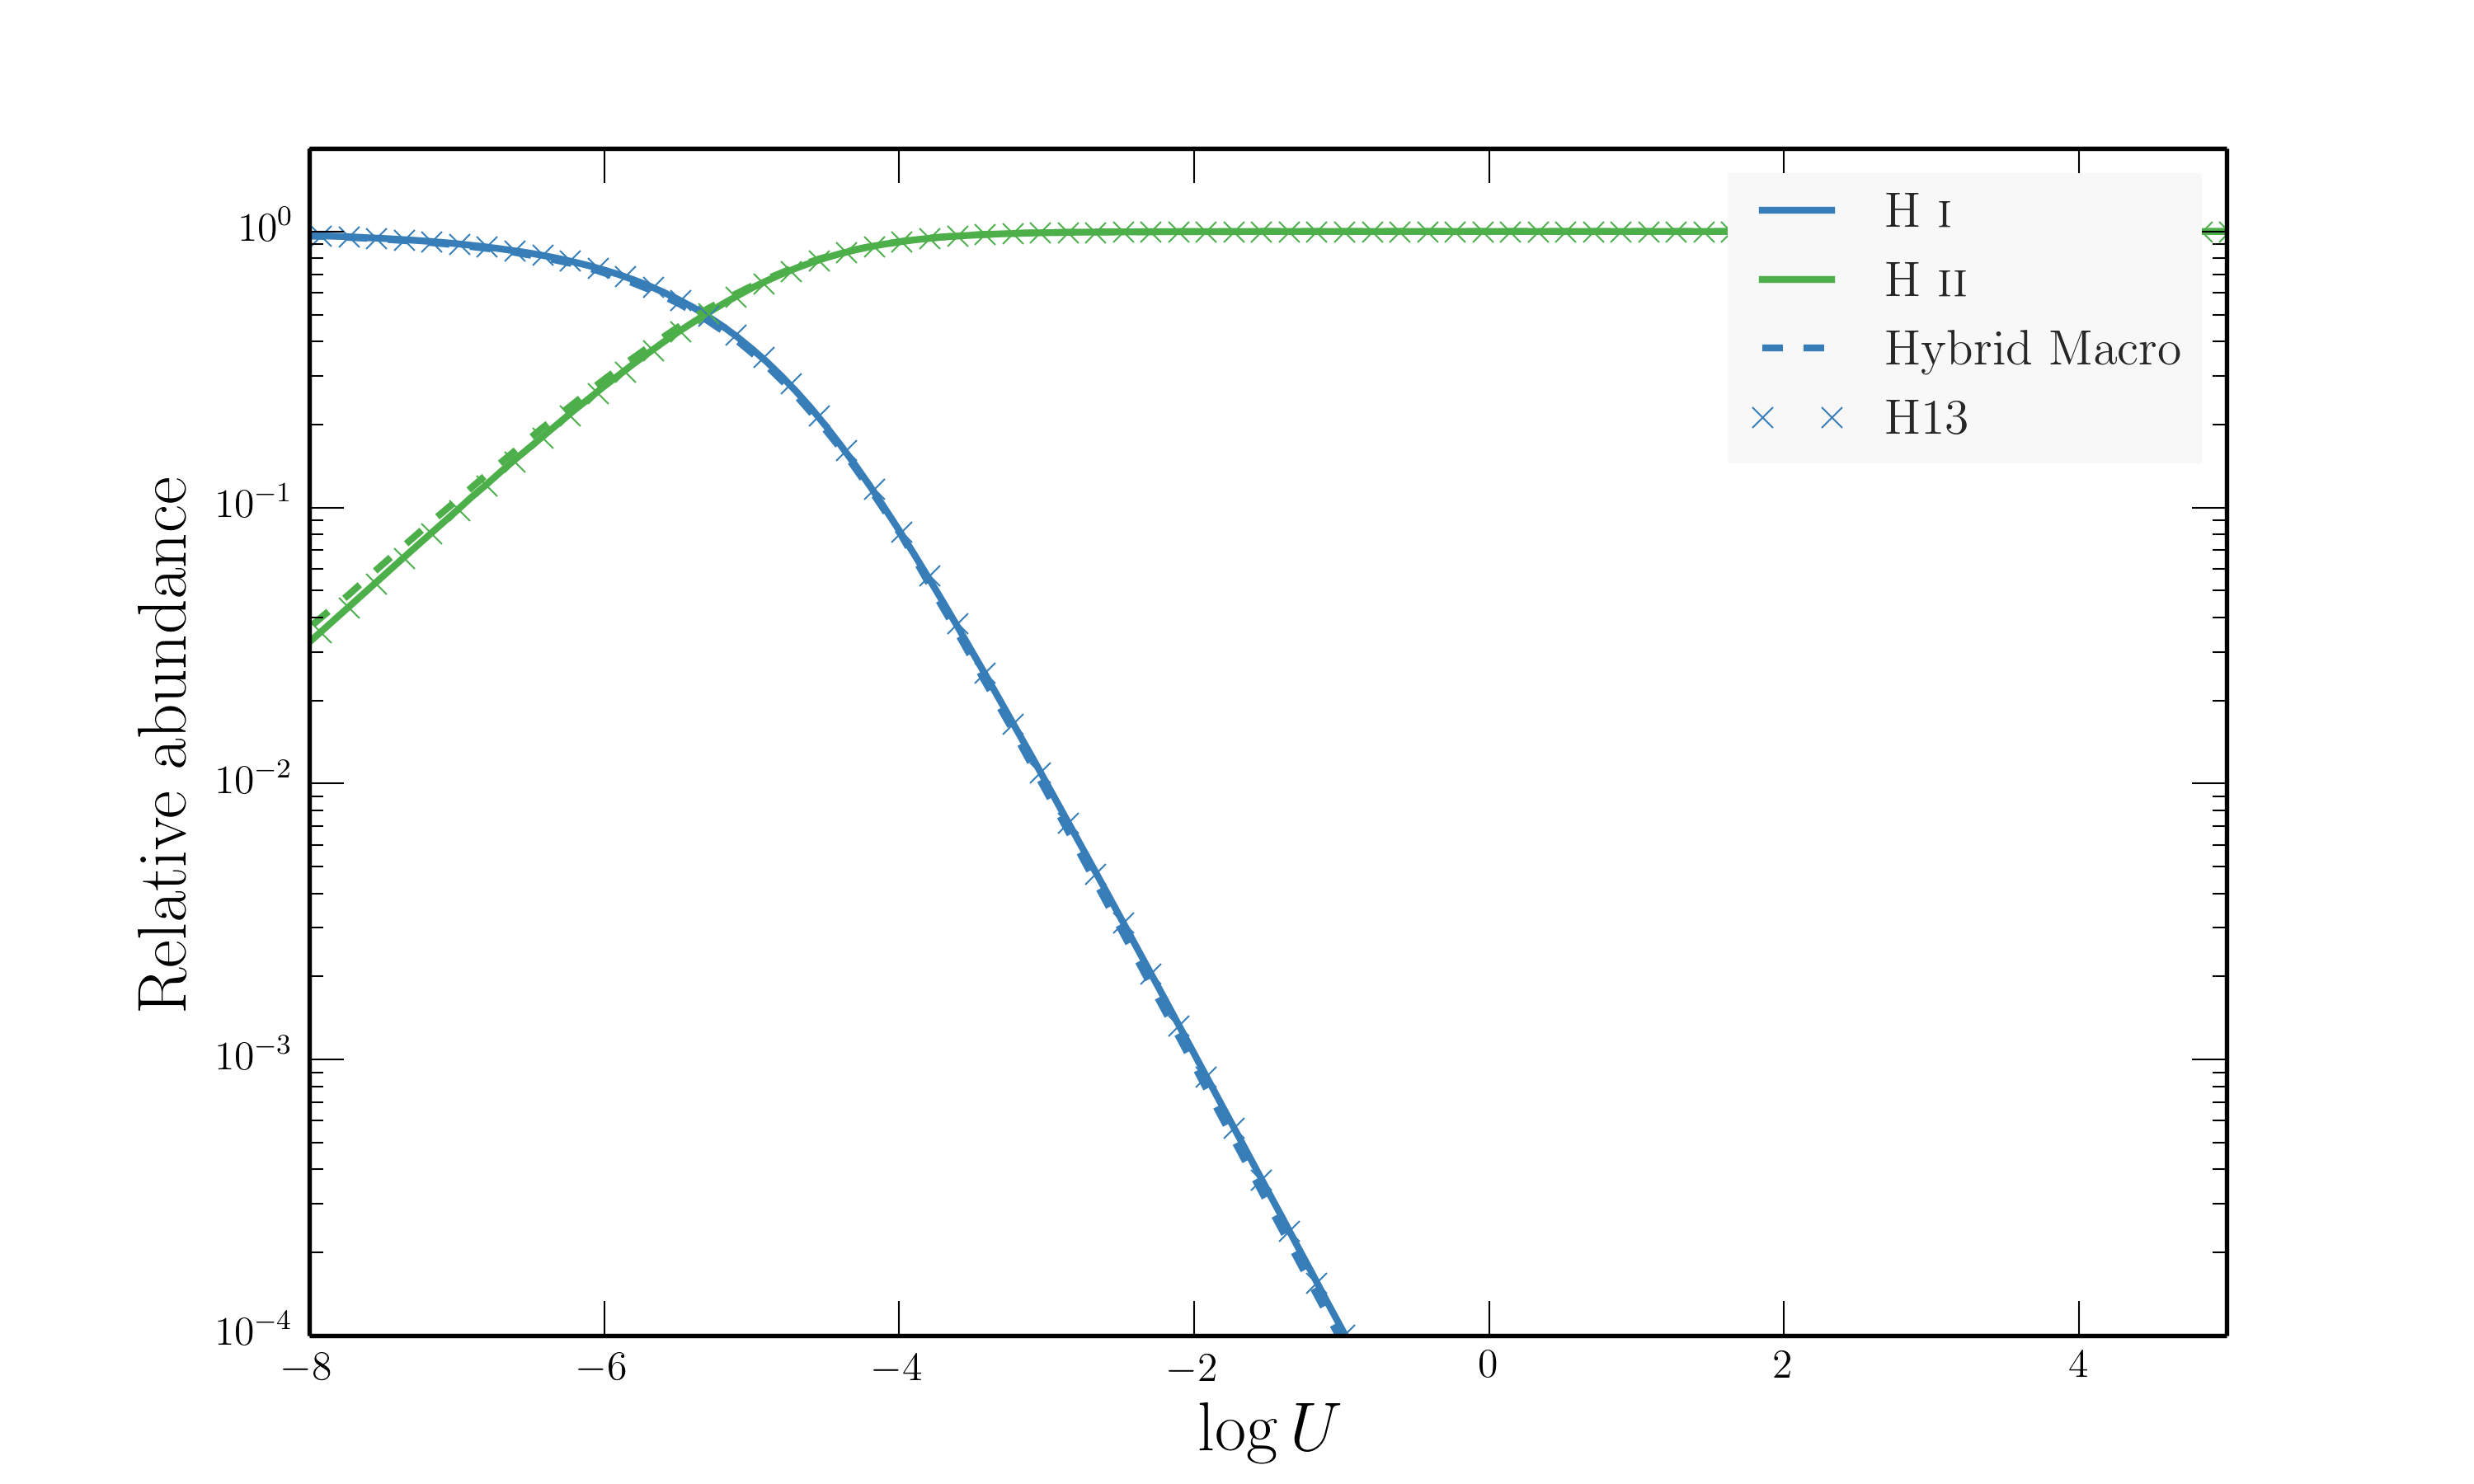
\includegraphics[width=1.0\textwidth]{figures/03-radtrans/hy_comp.png}
\caption
[Relative ion fractions for Hydrogen in \cld,\py\ in standard mode and 
\py\ in hybrid mode.]
{
Relative ion fractions as a function of ionization parameter from the
hybrid macro-atom scheme, with Hydrogen and Helium 
treated as a full macro-atom, compared
to both \cld\ and \py\ in simple-atom only mode.  
}
\label{fig:h_cloudy}
\end{figure}

\begin{figure}
\centering
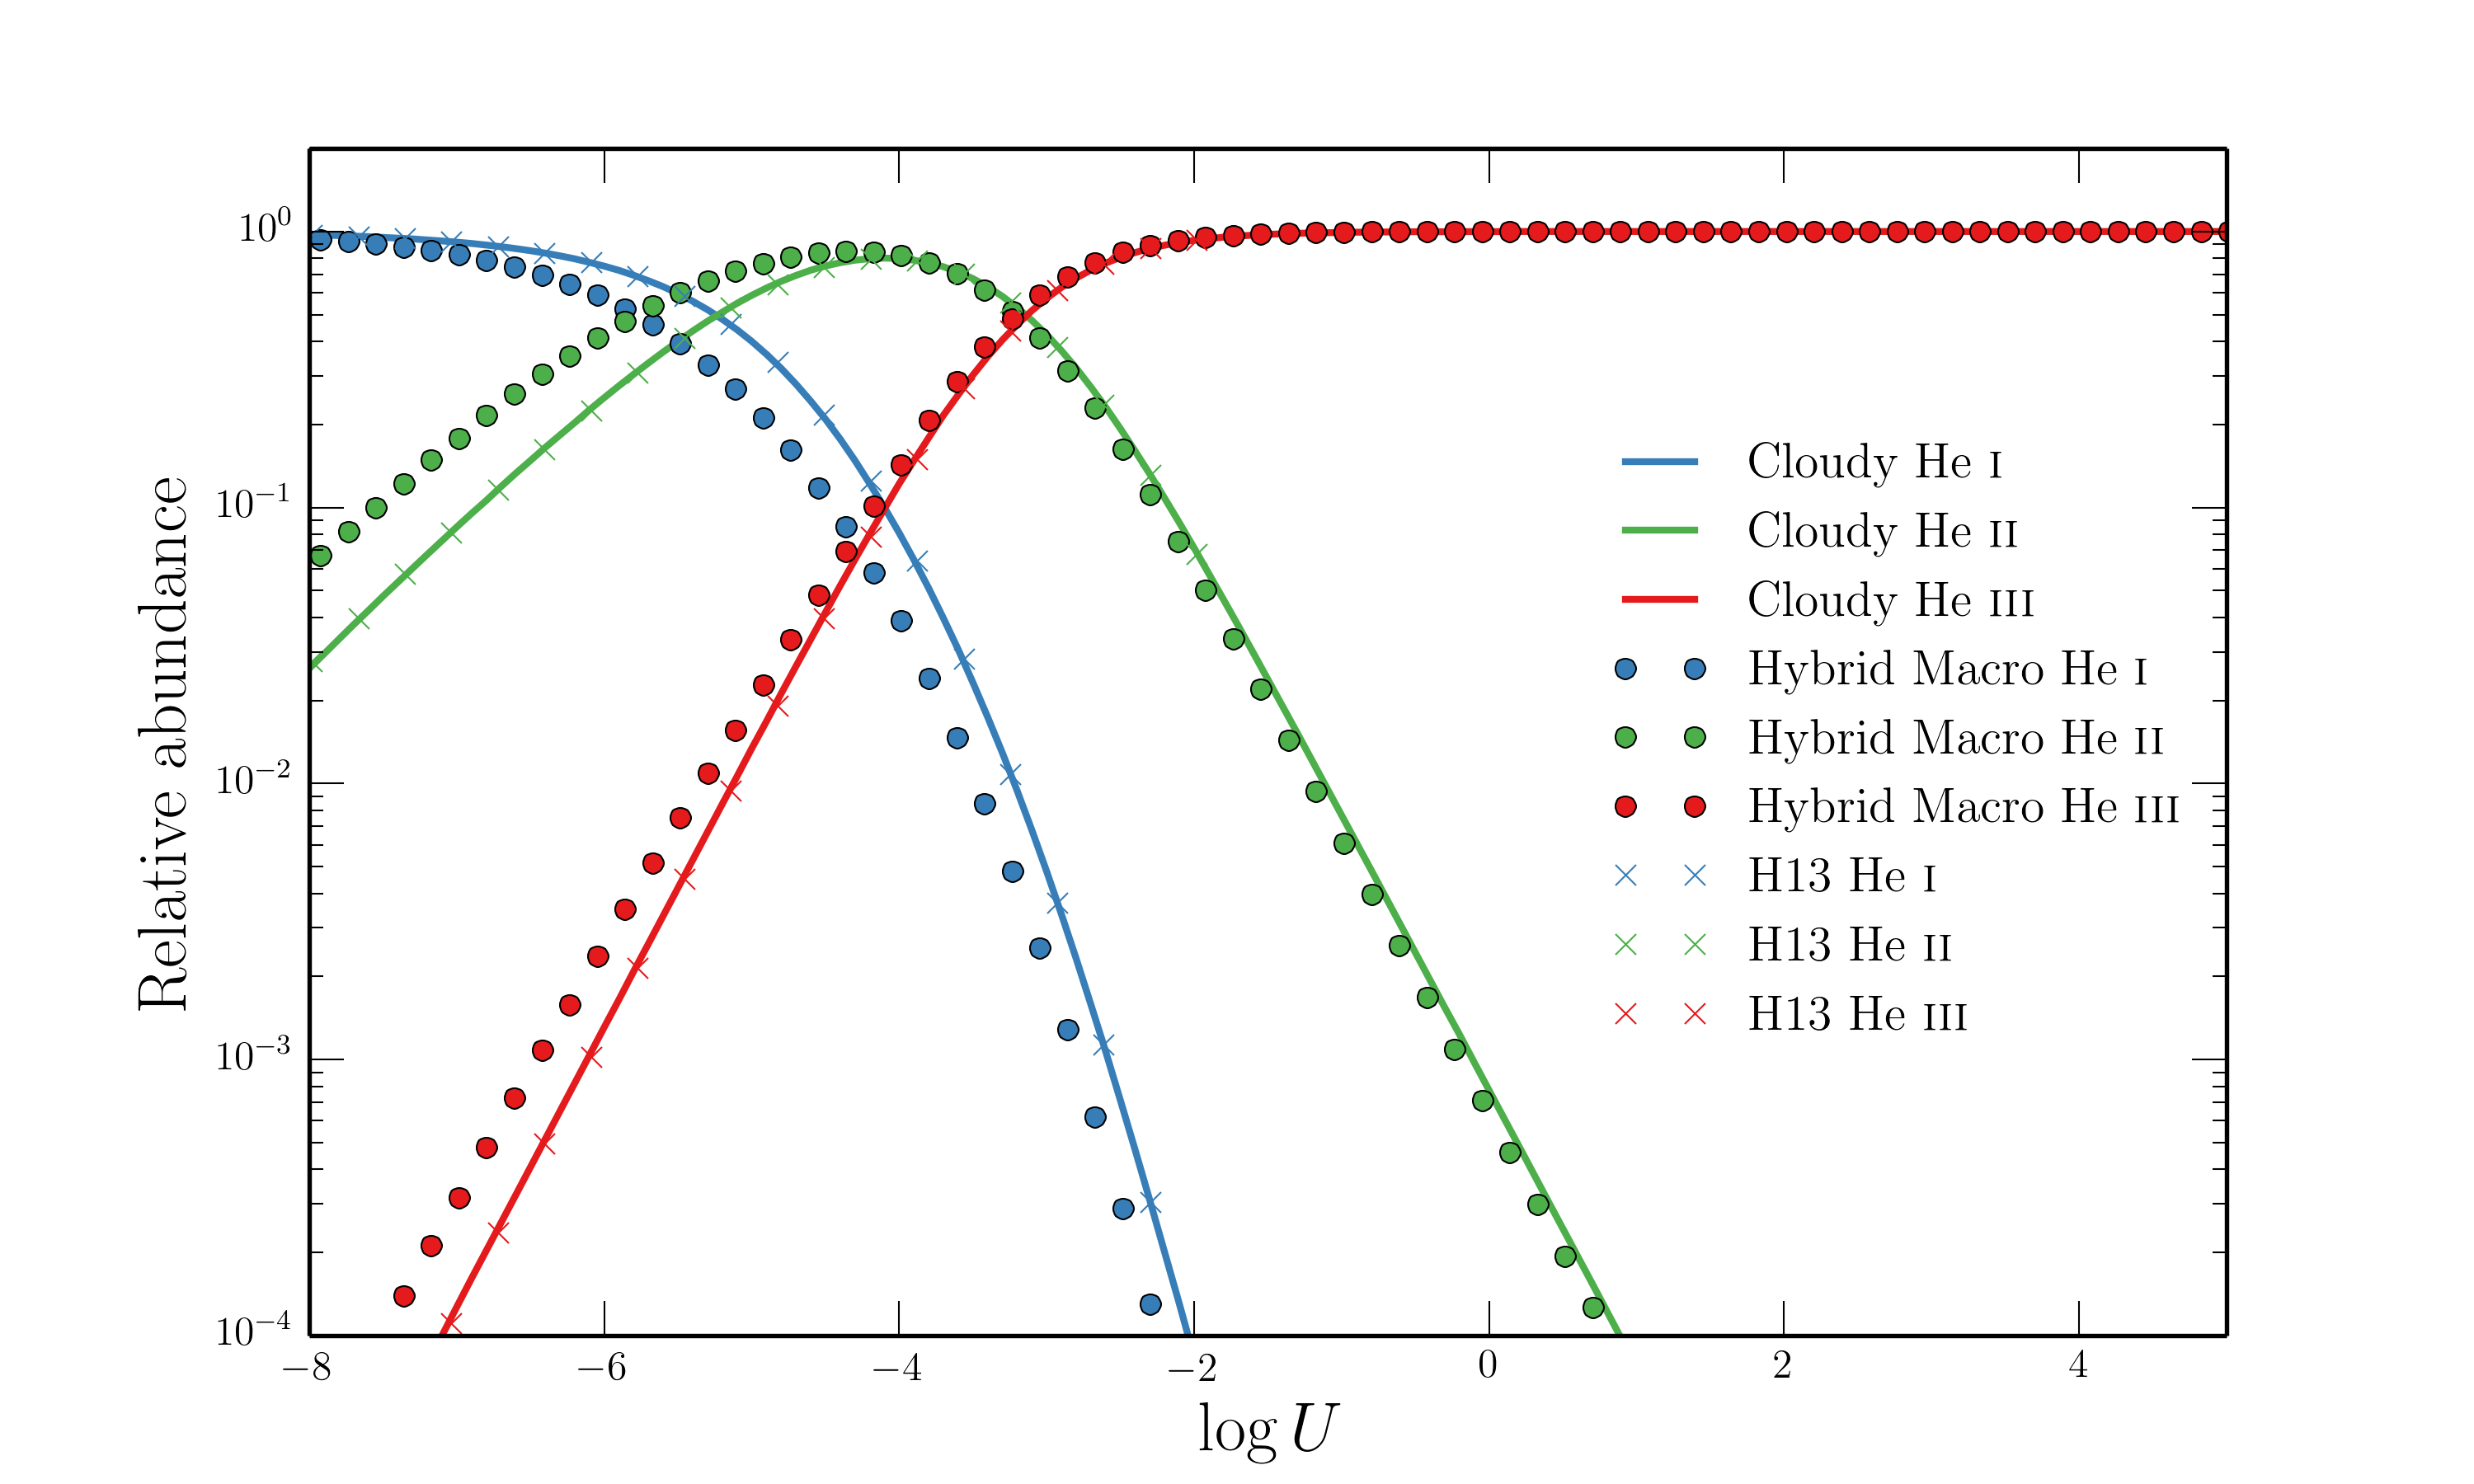
\includegraphics[width=1.0\textwidth]{figures/03-radtrans/he_comp.png}
\caption{
As figure~\ref{fig:h_cloudy}, but for Helium.
}
\label{fig:he_cloudy}
\end{figure}

\begin{figure}
\centering
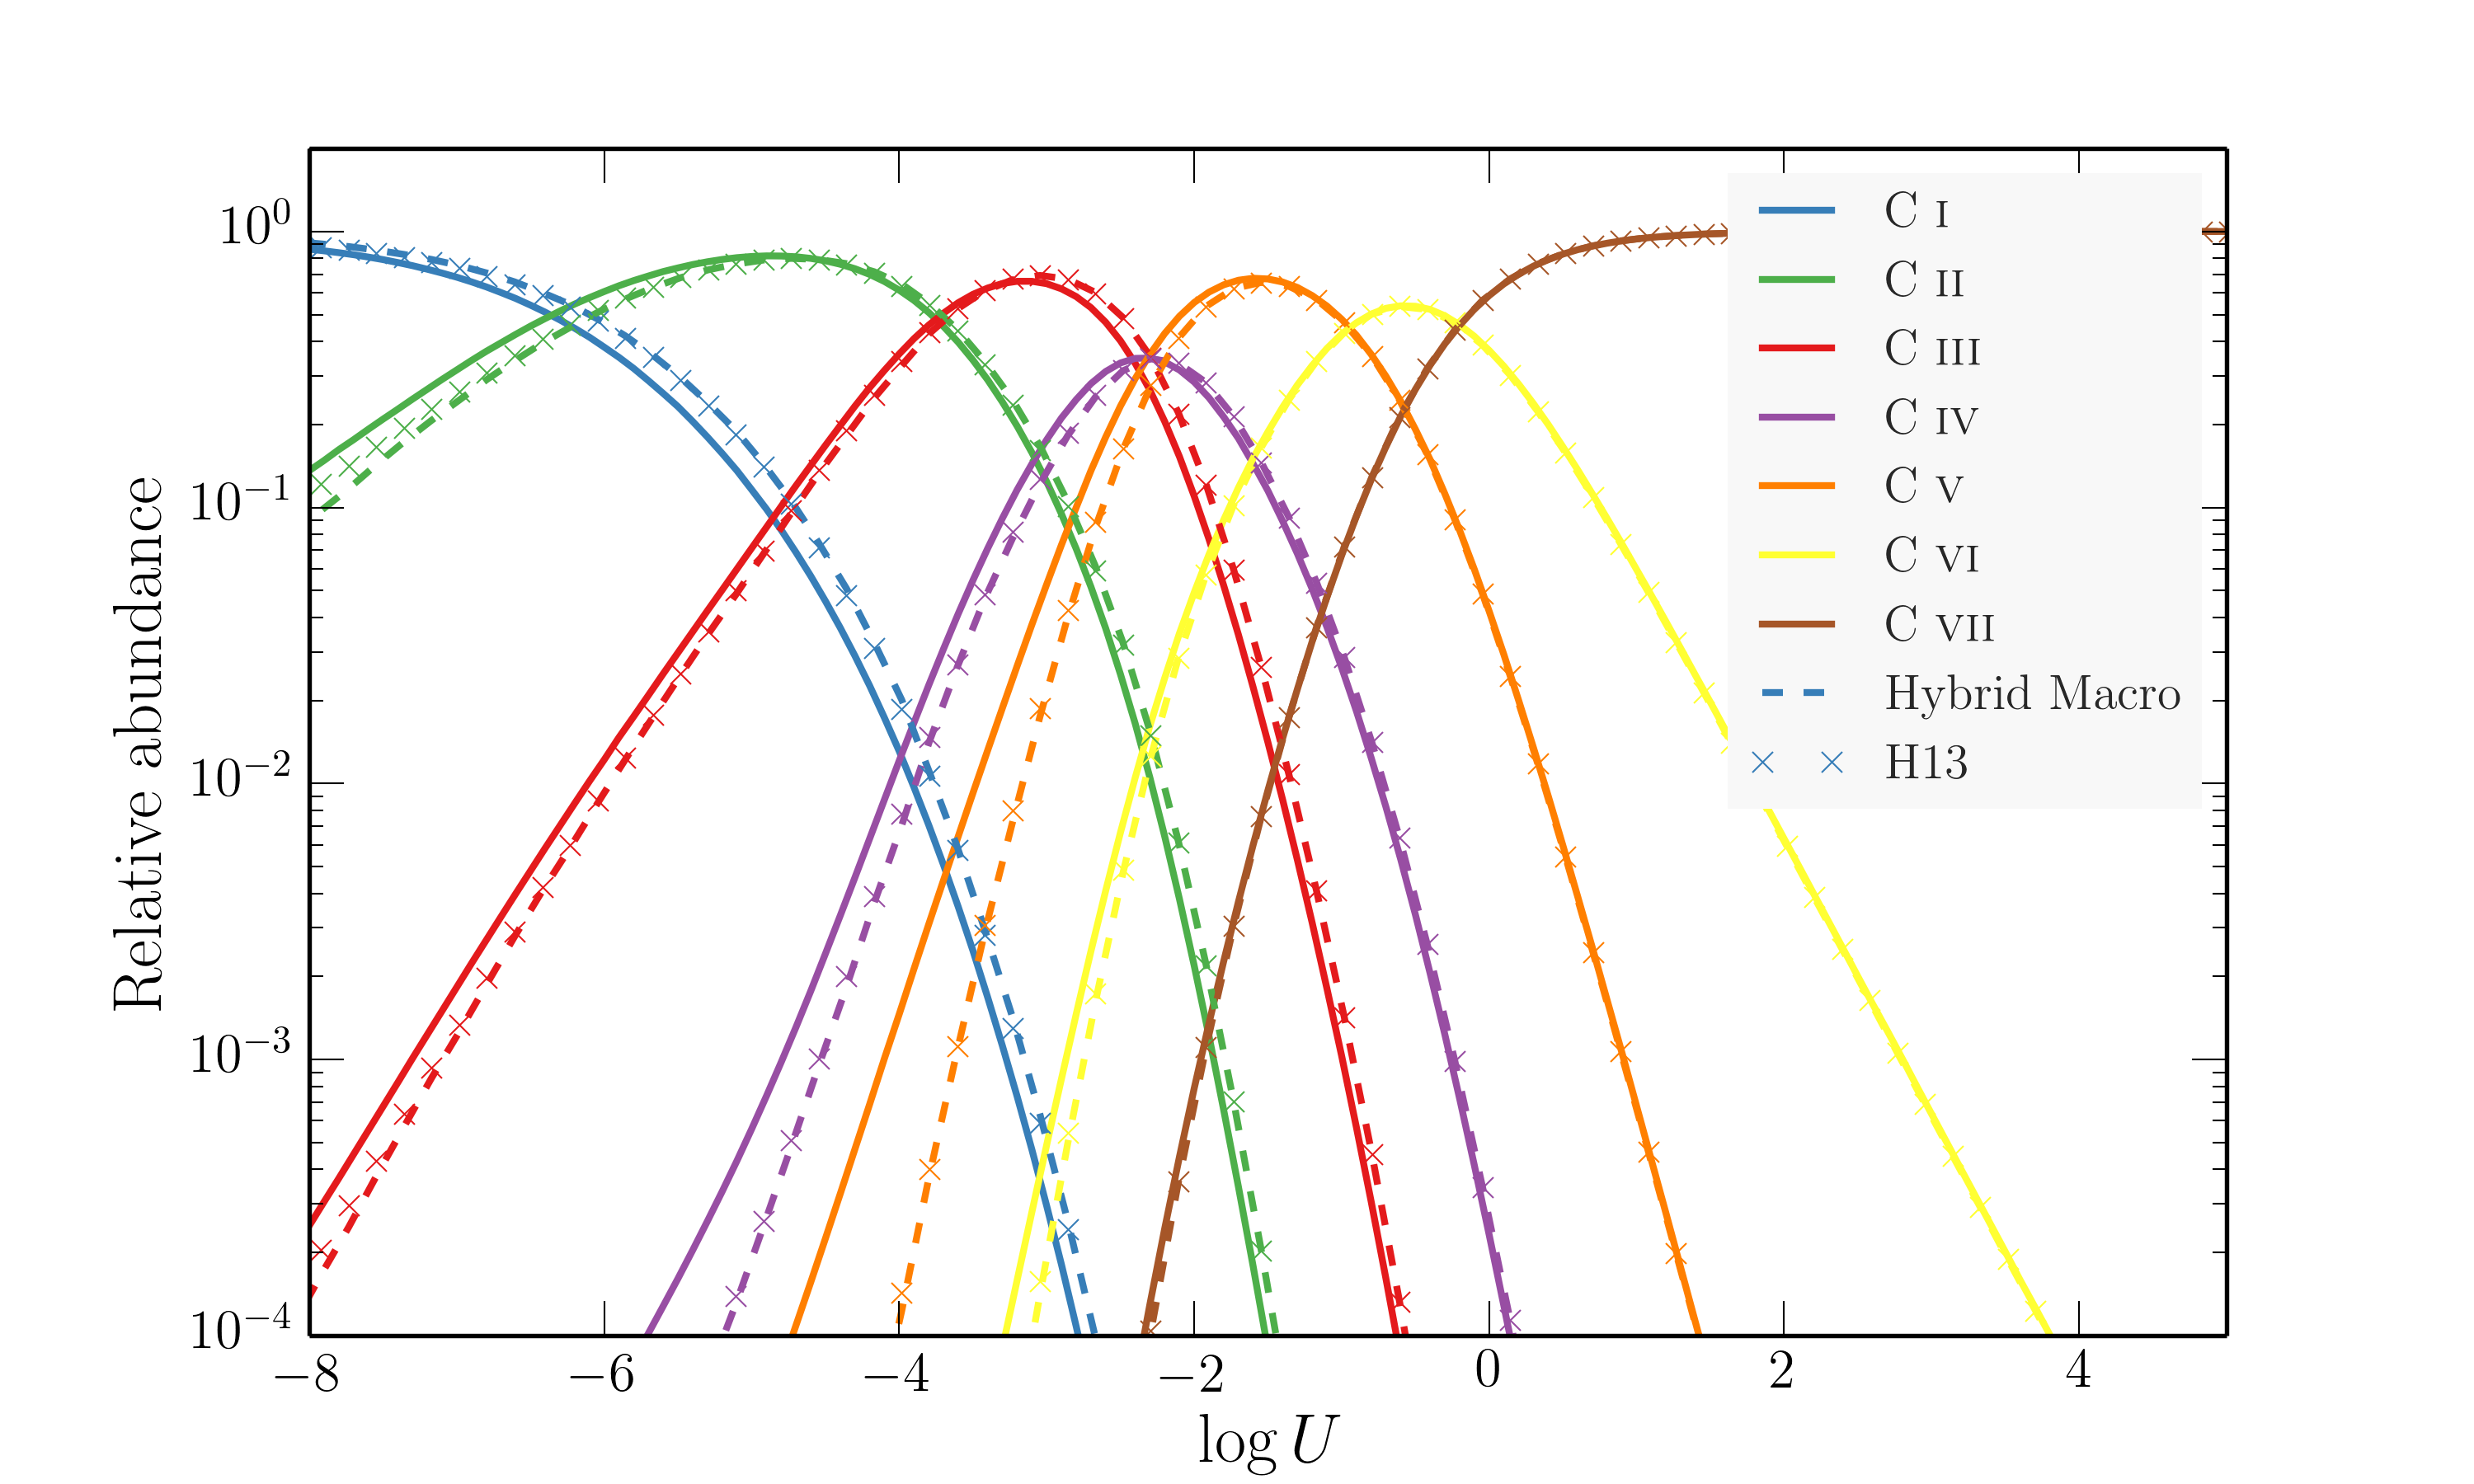
\includegraphics[width=1.0\textwidth]{figures/03-radtrans/ca_comp.png}
\caption
{
As figure~\ref{fig:h_cloudy}, but for Carbon.
}
\label{fig:c_cloudy}
\end{figure}

\begin{figure}
\centering
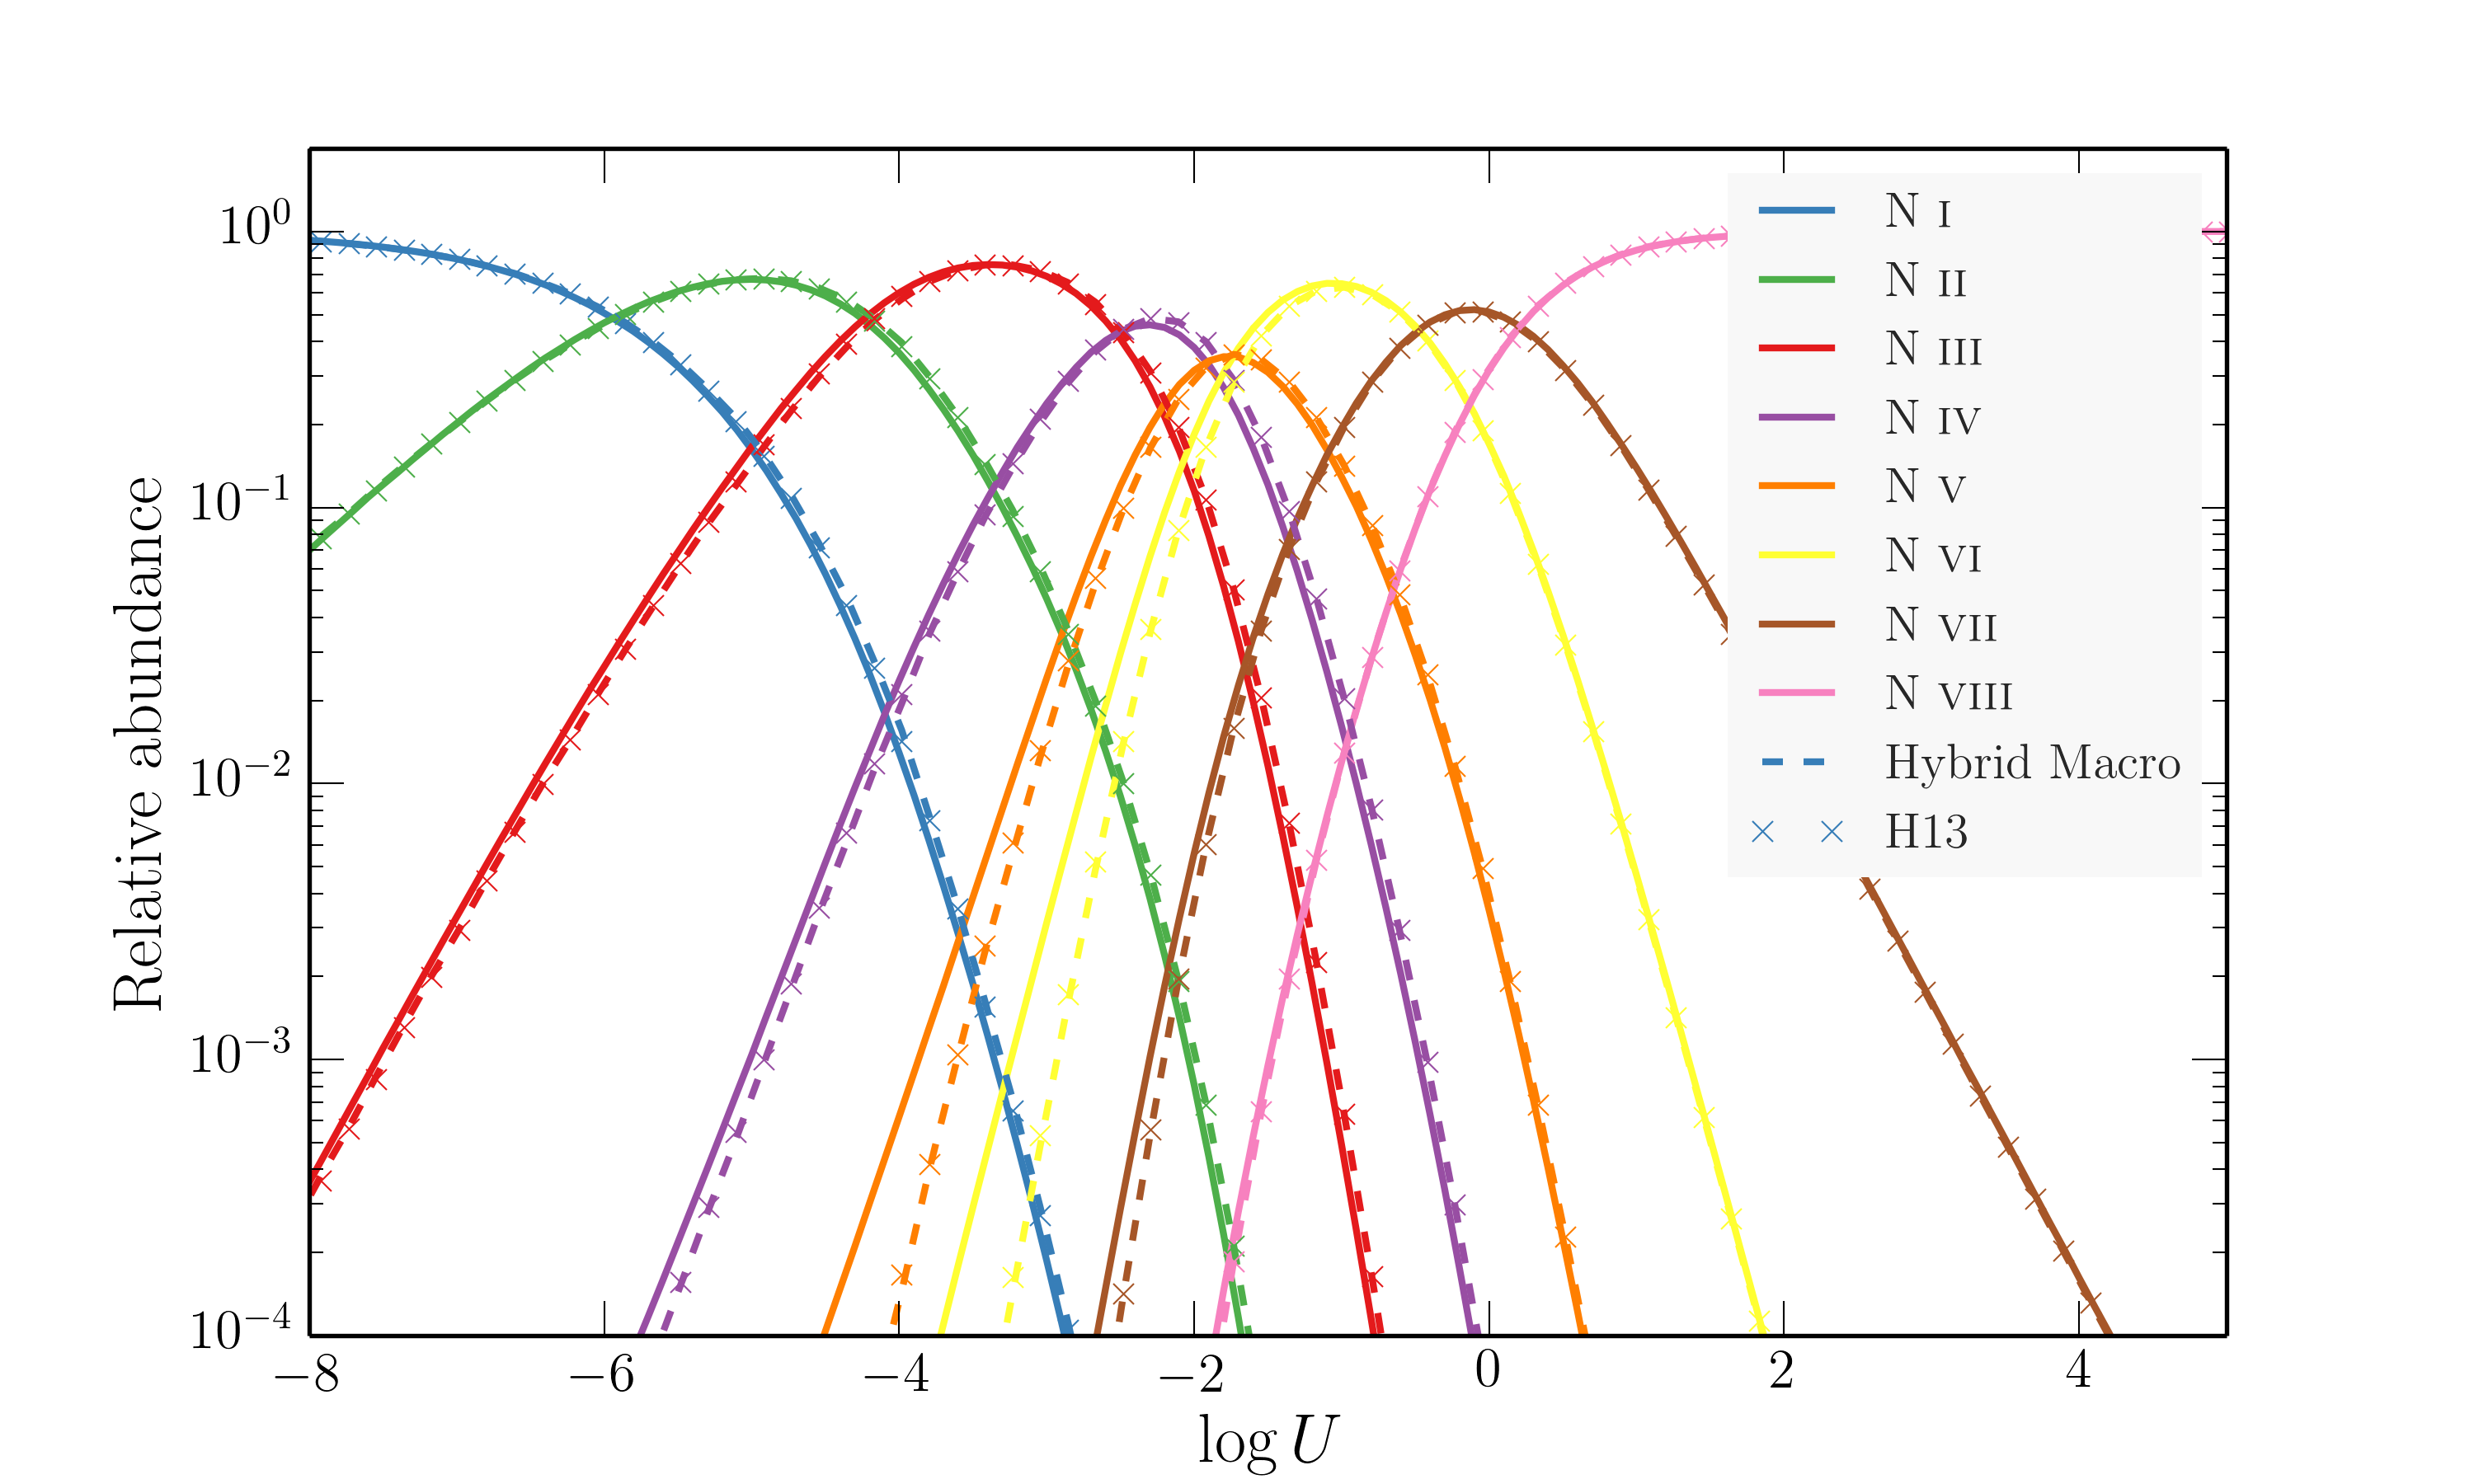
\includegraphics[width=1.0\textwidth]{figures/03-radtrans/ni_comp.png}
\caption{
As figure~\ref{fig:h_cloudy}, but for Nitrogen.
}
\label{fig:n_cloudy}
\end{figure}

\begin{figure}
\centering
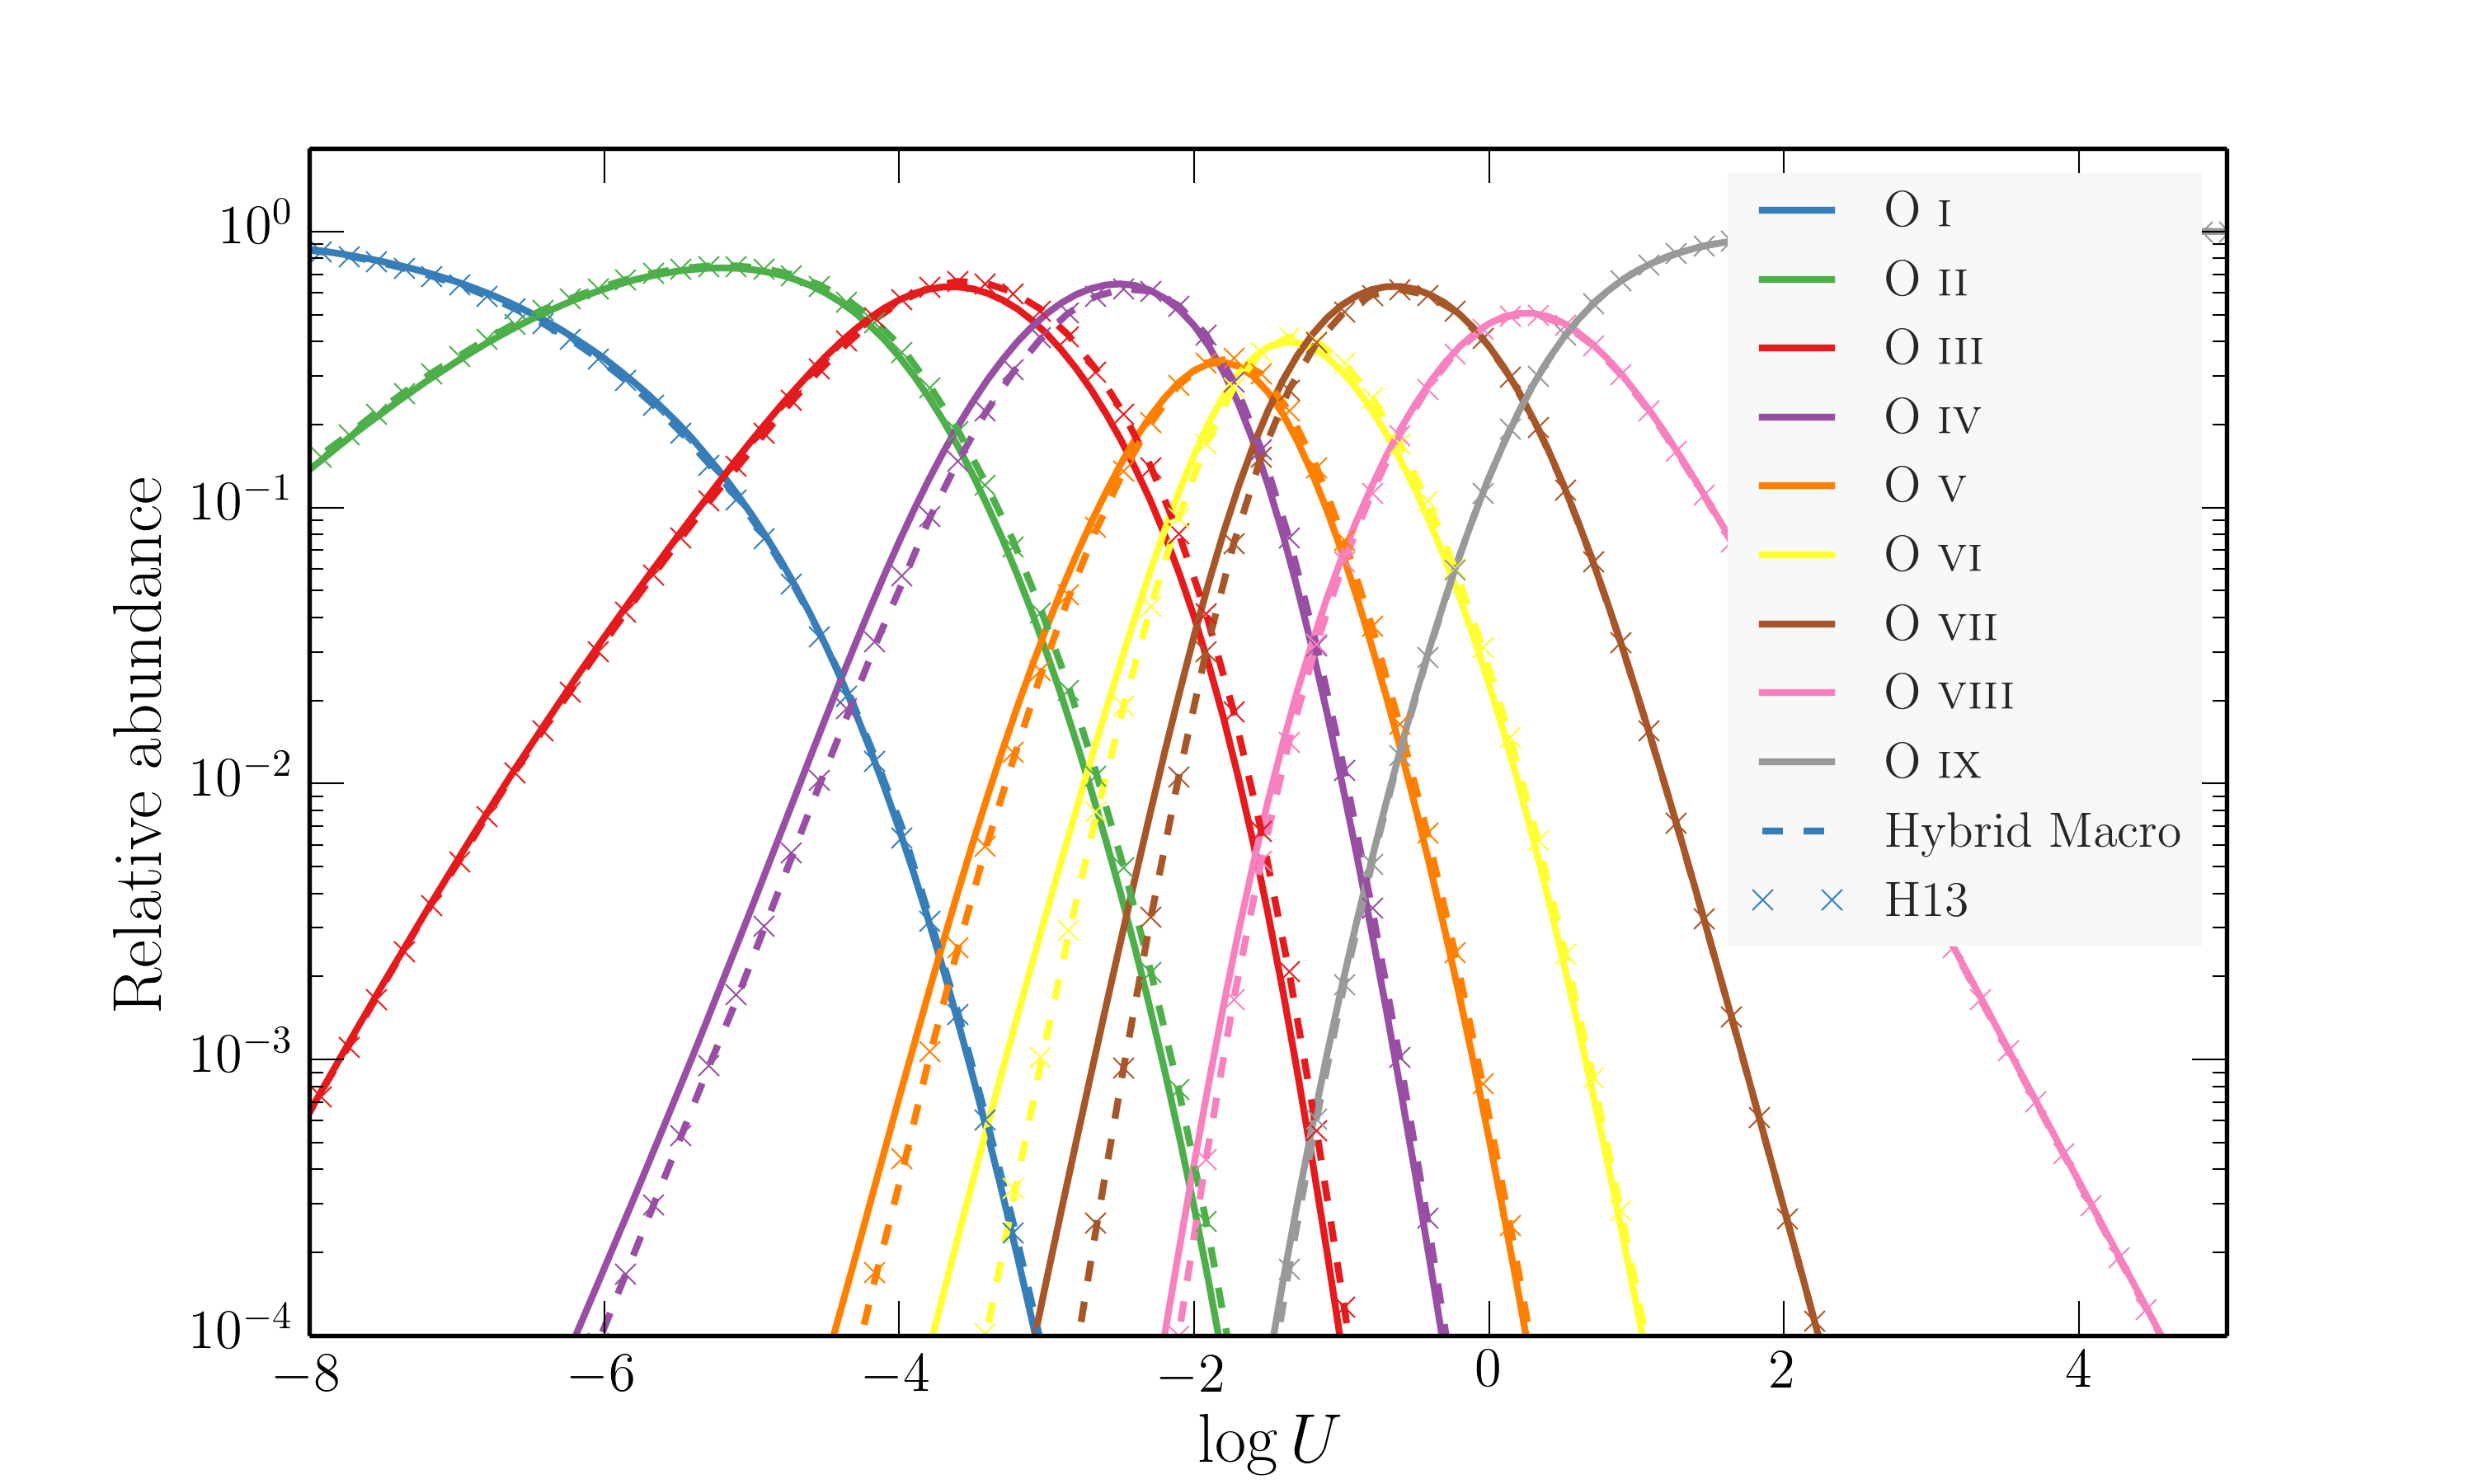
\includegraphics[width=1.0\textwidth]{figures/03-radtrans/ox_comp.png}
\caption
{
As figure~\ref{fig:h_cloudy}, but for Oxygen.
}
\label{fig:ox_cloudy}
\end{figure}

\begin{figure}
\centering
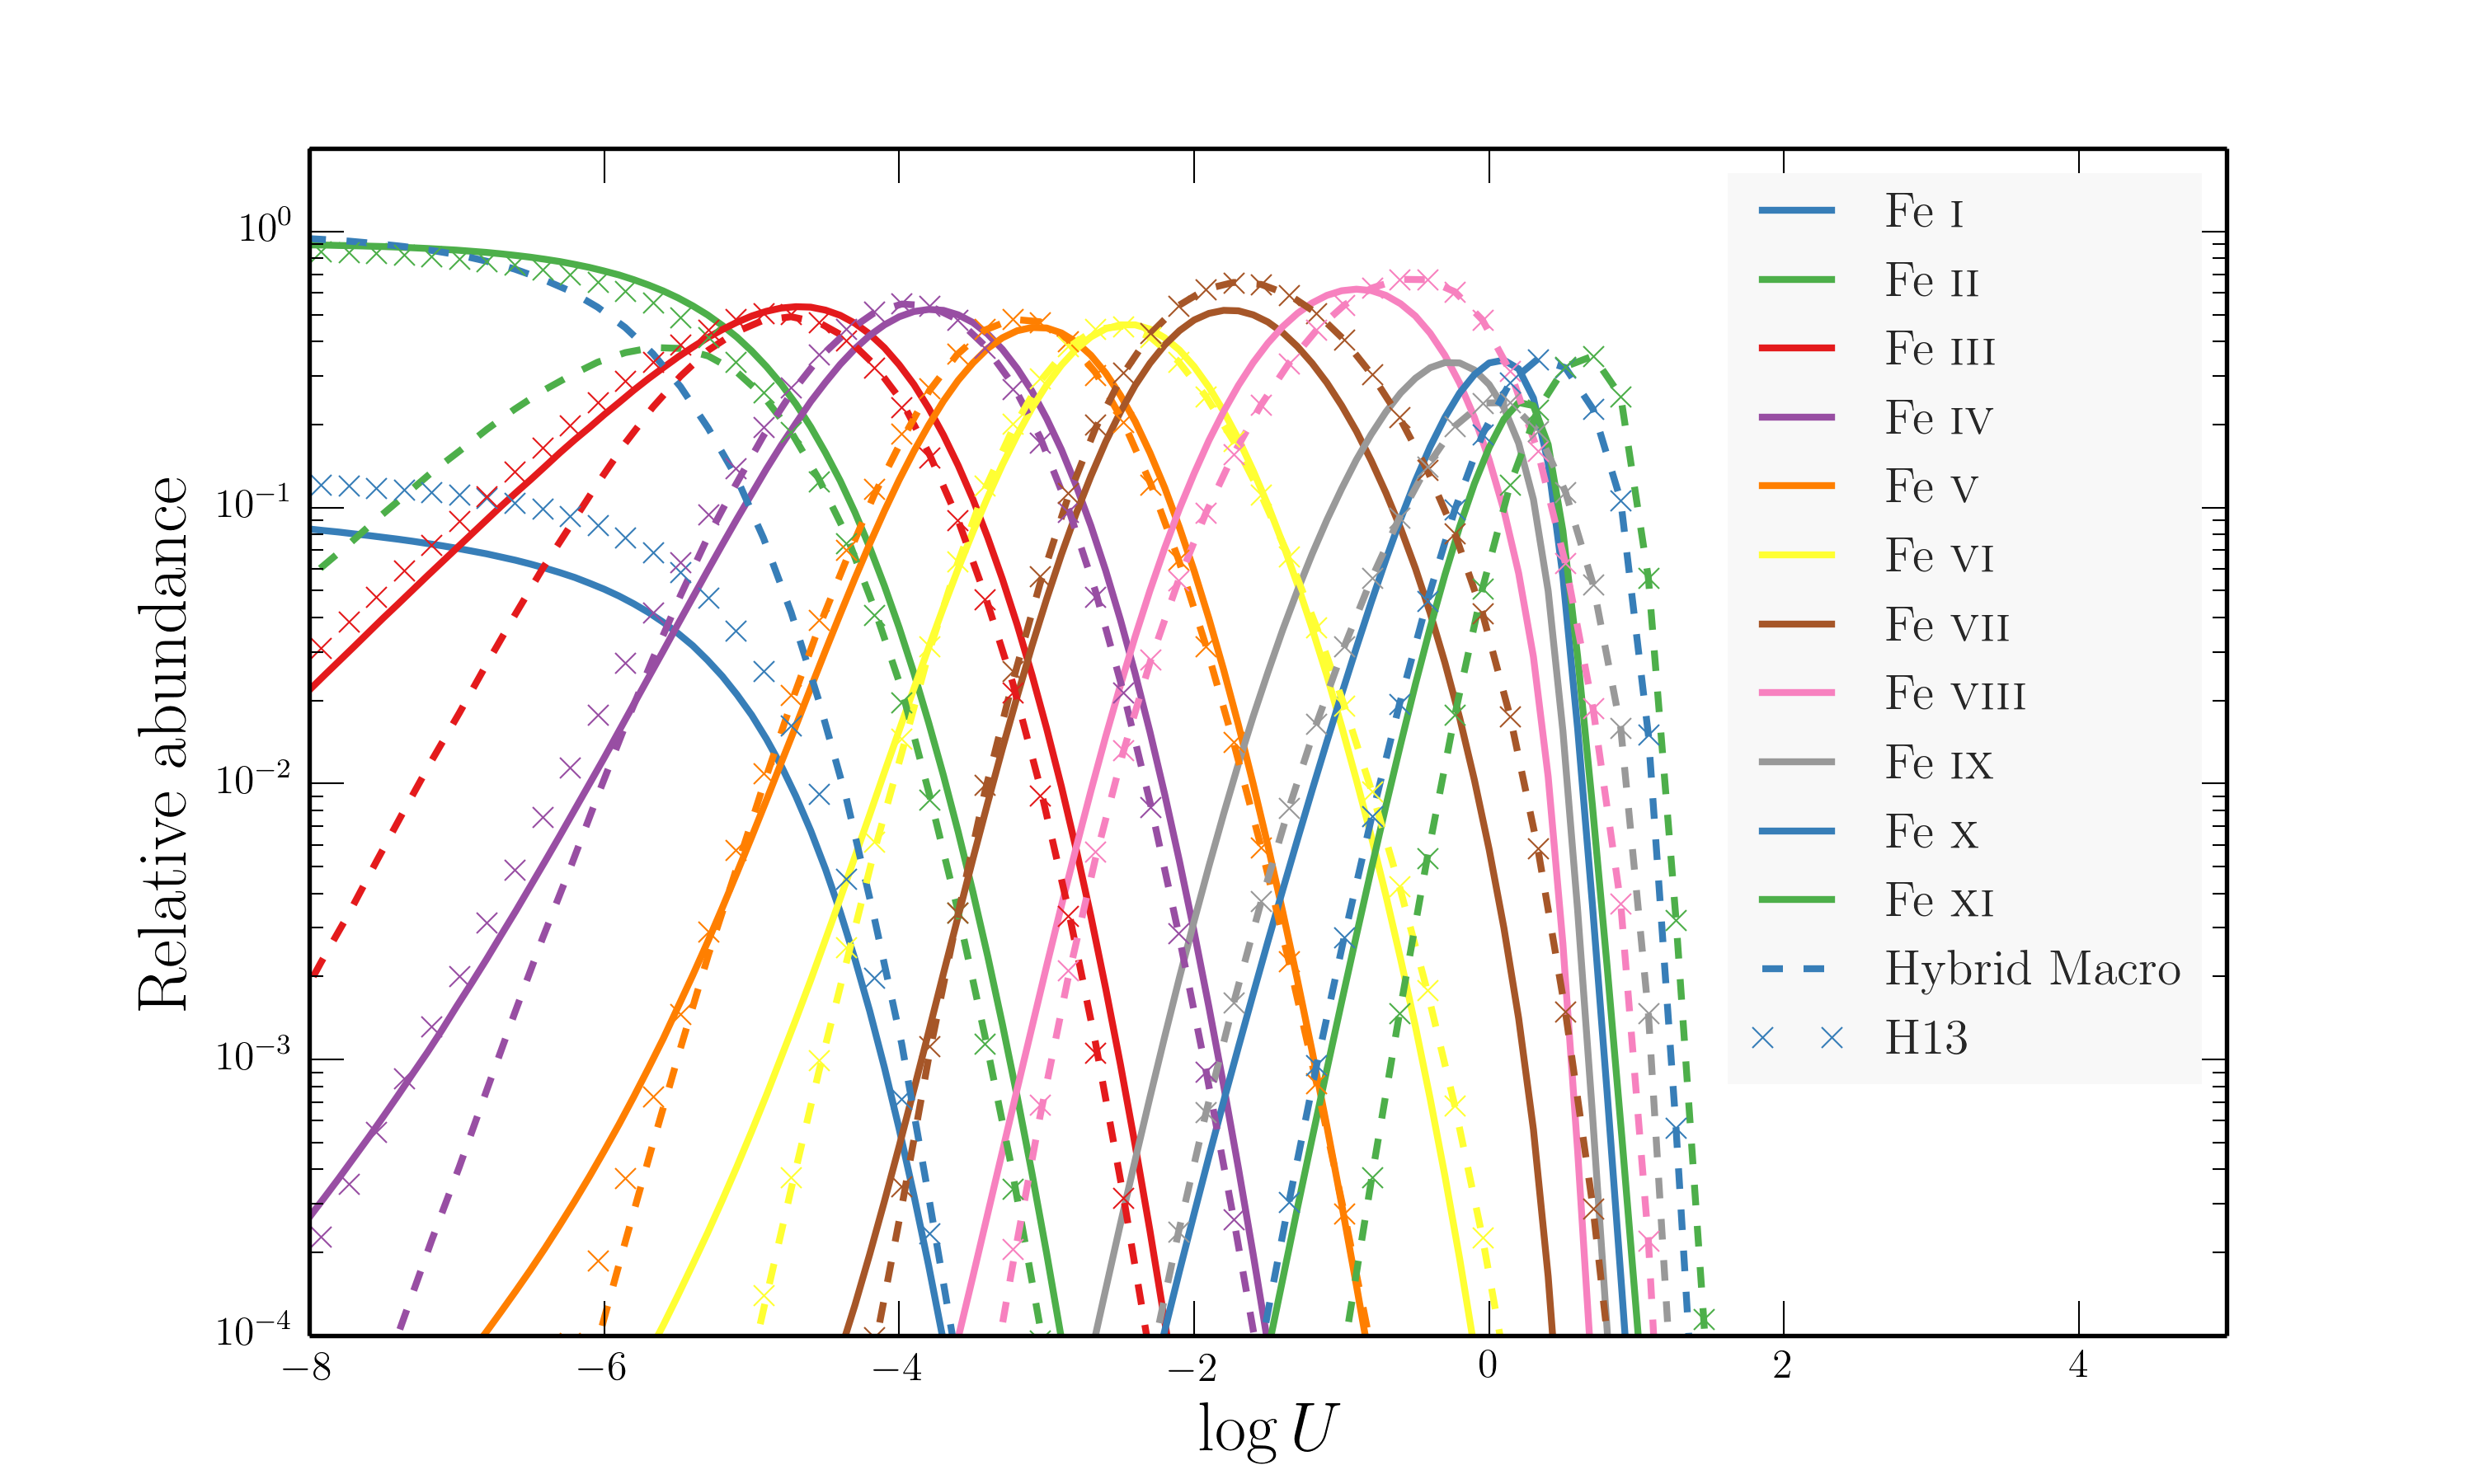
\includegraphics[width=1.0\textwidth]{figures/03-radtrans/ir_comp.png}
\caption
{
As figure~\ref{fig:h_cloudy}, but for the first 11 ionization stages of Iron.
}
\label{fig:ir_cloudy}
\end{figure}

\subsection{Macro-atom Testing Against \tar\ and Theory}

\tar\ is a 1D photoionization and radiative transfer designed to
model SNe in a quick and easy python package, and is described in detail by
\cite{kerzendorfsim}. Although \tar\ is simpler in terms
of geometry, it has many of the same capabilities of \py\ and 
thus makes for an excellent comparison. 

Fig.~\ref{fig:caseb_tests} shows the results of two code tests. 
In the top panel, I show a comparison of the Balmer series 
emissivities as predicted by \py\ in the l-mixed Case~B limit against the
analytical calculations by \cite{seaton1959}. 
Both calculations are calculated at $T_e=10,000$K.
Case B is an approximation commonly used in nebular astrophysics 
\citep[see e.g.][]{osterbrock} in which
one assumes that all line transitions are optically thin, except
for the \la\ transition, which is taken as optically thick.
Thus, this test comparison is carried out using a thin shell
of plasma in which the escape probabilities, $\beta_{uj}$ 
are artificially set to 1 in all transitions except \la, which
has its $\beta_{uj}$ set to 0.

The bottom panel shows a comparison of He I level populations 
(the most complex ion currently 
treated as a macro-atom) between \py\ and \tar\ models.
The calculation is conducted with physical parameters of $n_e=5.96\times10^4$~cm$^{-3}$,
$T_e=30,600$K, $T_R=43,482$K and $W=9.65\times10^{-5}$. 
Considering the two codes use different atomic data and 
\tar, unlike \py, currently has a 
complete treatment of collisions between 
radiatively forbidden transitions, the factor of 
$<2$ agreement is encouraging. 

\begin{figure}
\centering
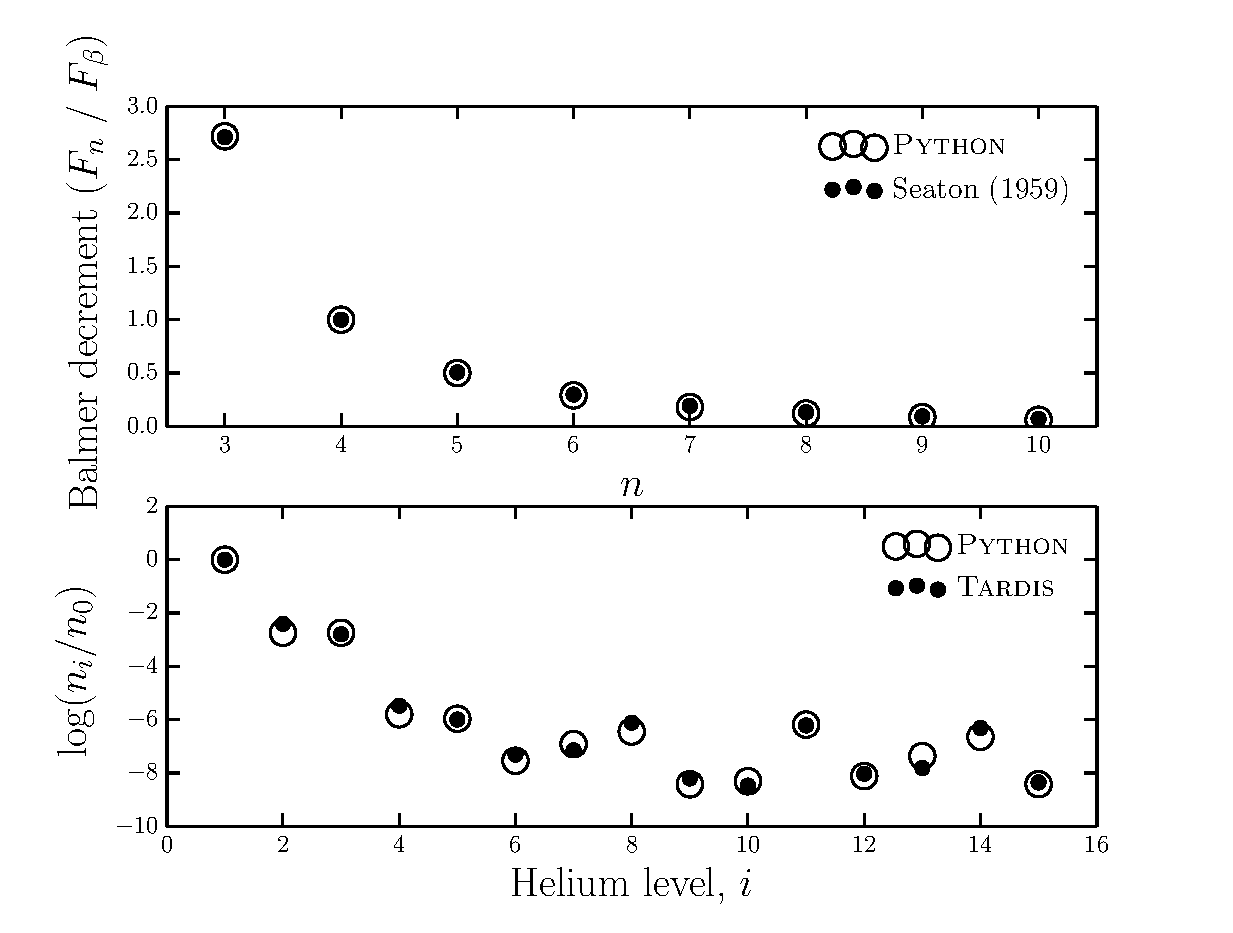
\includegraphics[width=1.0\textwidth]{figures/05-cvpaper/fig_caseb_tardis.eps}
\caption
[Balmer decrements in \py\ compared to Seaton (1959), and He level populations
compared to \tar.]
{
{\sl Top Panel:} `Case B' Balmer decrements computed 
with \py\ compared to analytic calculations
by Seaton (1959). Both calculations are calculated at $T_e=10,000$K.
{\sl Bottom Panel:}  a comparison of He I level populations (the most complex ion we currently 
treat as a macro-atom) between \py\ and \tar\ models. 
The calculation is conducted in thin shell mode
with physical parameters of $n_e=5.96\times10^4$~cm$^{-3}$,
$T_e=30,600$K, $T_R=43,482$K and $W=9.65\times10^{-5}$. 
}
\label{fig:caseb_tests}
\end{figure}

Fig.~\ref{fig:tardis_spec} shows a comparison 
between \tar\ and \py\ synthetic spectra from 
a simple 1D SN model. This comparison was originally presented by
\cite{kerzendorfsim}, but I have since then discovered a bug in the Doppler shifting
routine in \py, introduced around \py\ 76, which was present in this test. 
Fixing this issue leads to slightly better agreement between the two codes. 
The model involves a full computation of the ionization state in the 
ML93 mode, and, although run in 1D, still tests most of the radiative transfer
machinery of the code. The spectra are in good agreement, considering
there are differences in their excitation treatments and atomic data.
This comparison is particular encouraging when we consider
that \cite{kerzendorfsim} also show comparisons with other SN codes such
as \textsc{Artis} \citep{kromersim2009}.

\begin{figure}
\centering
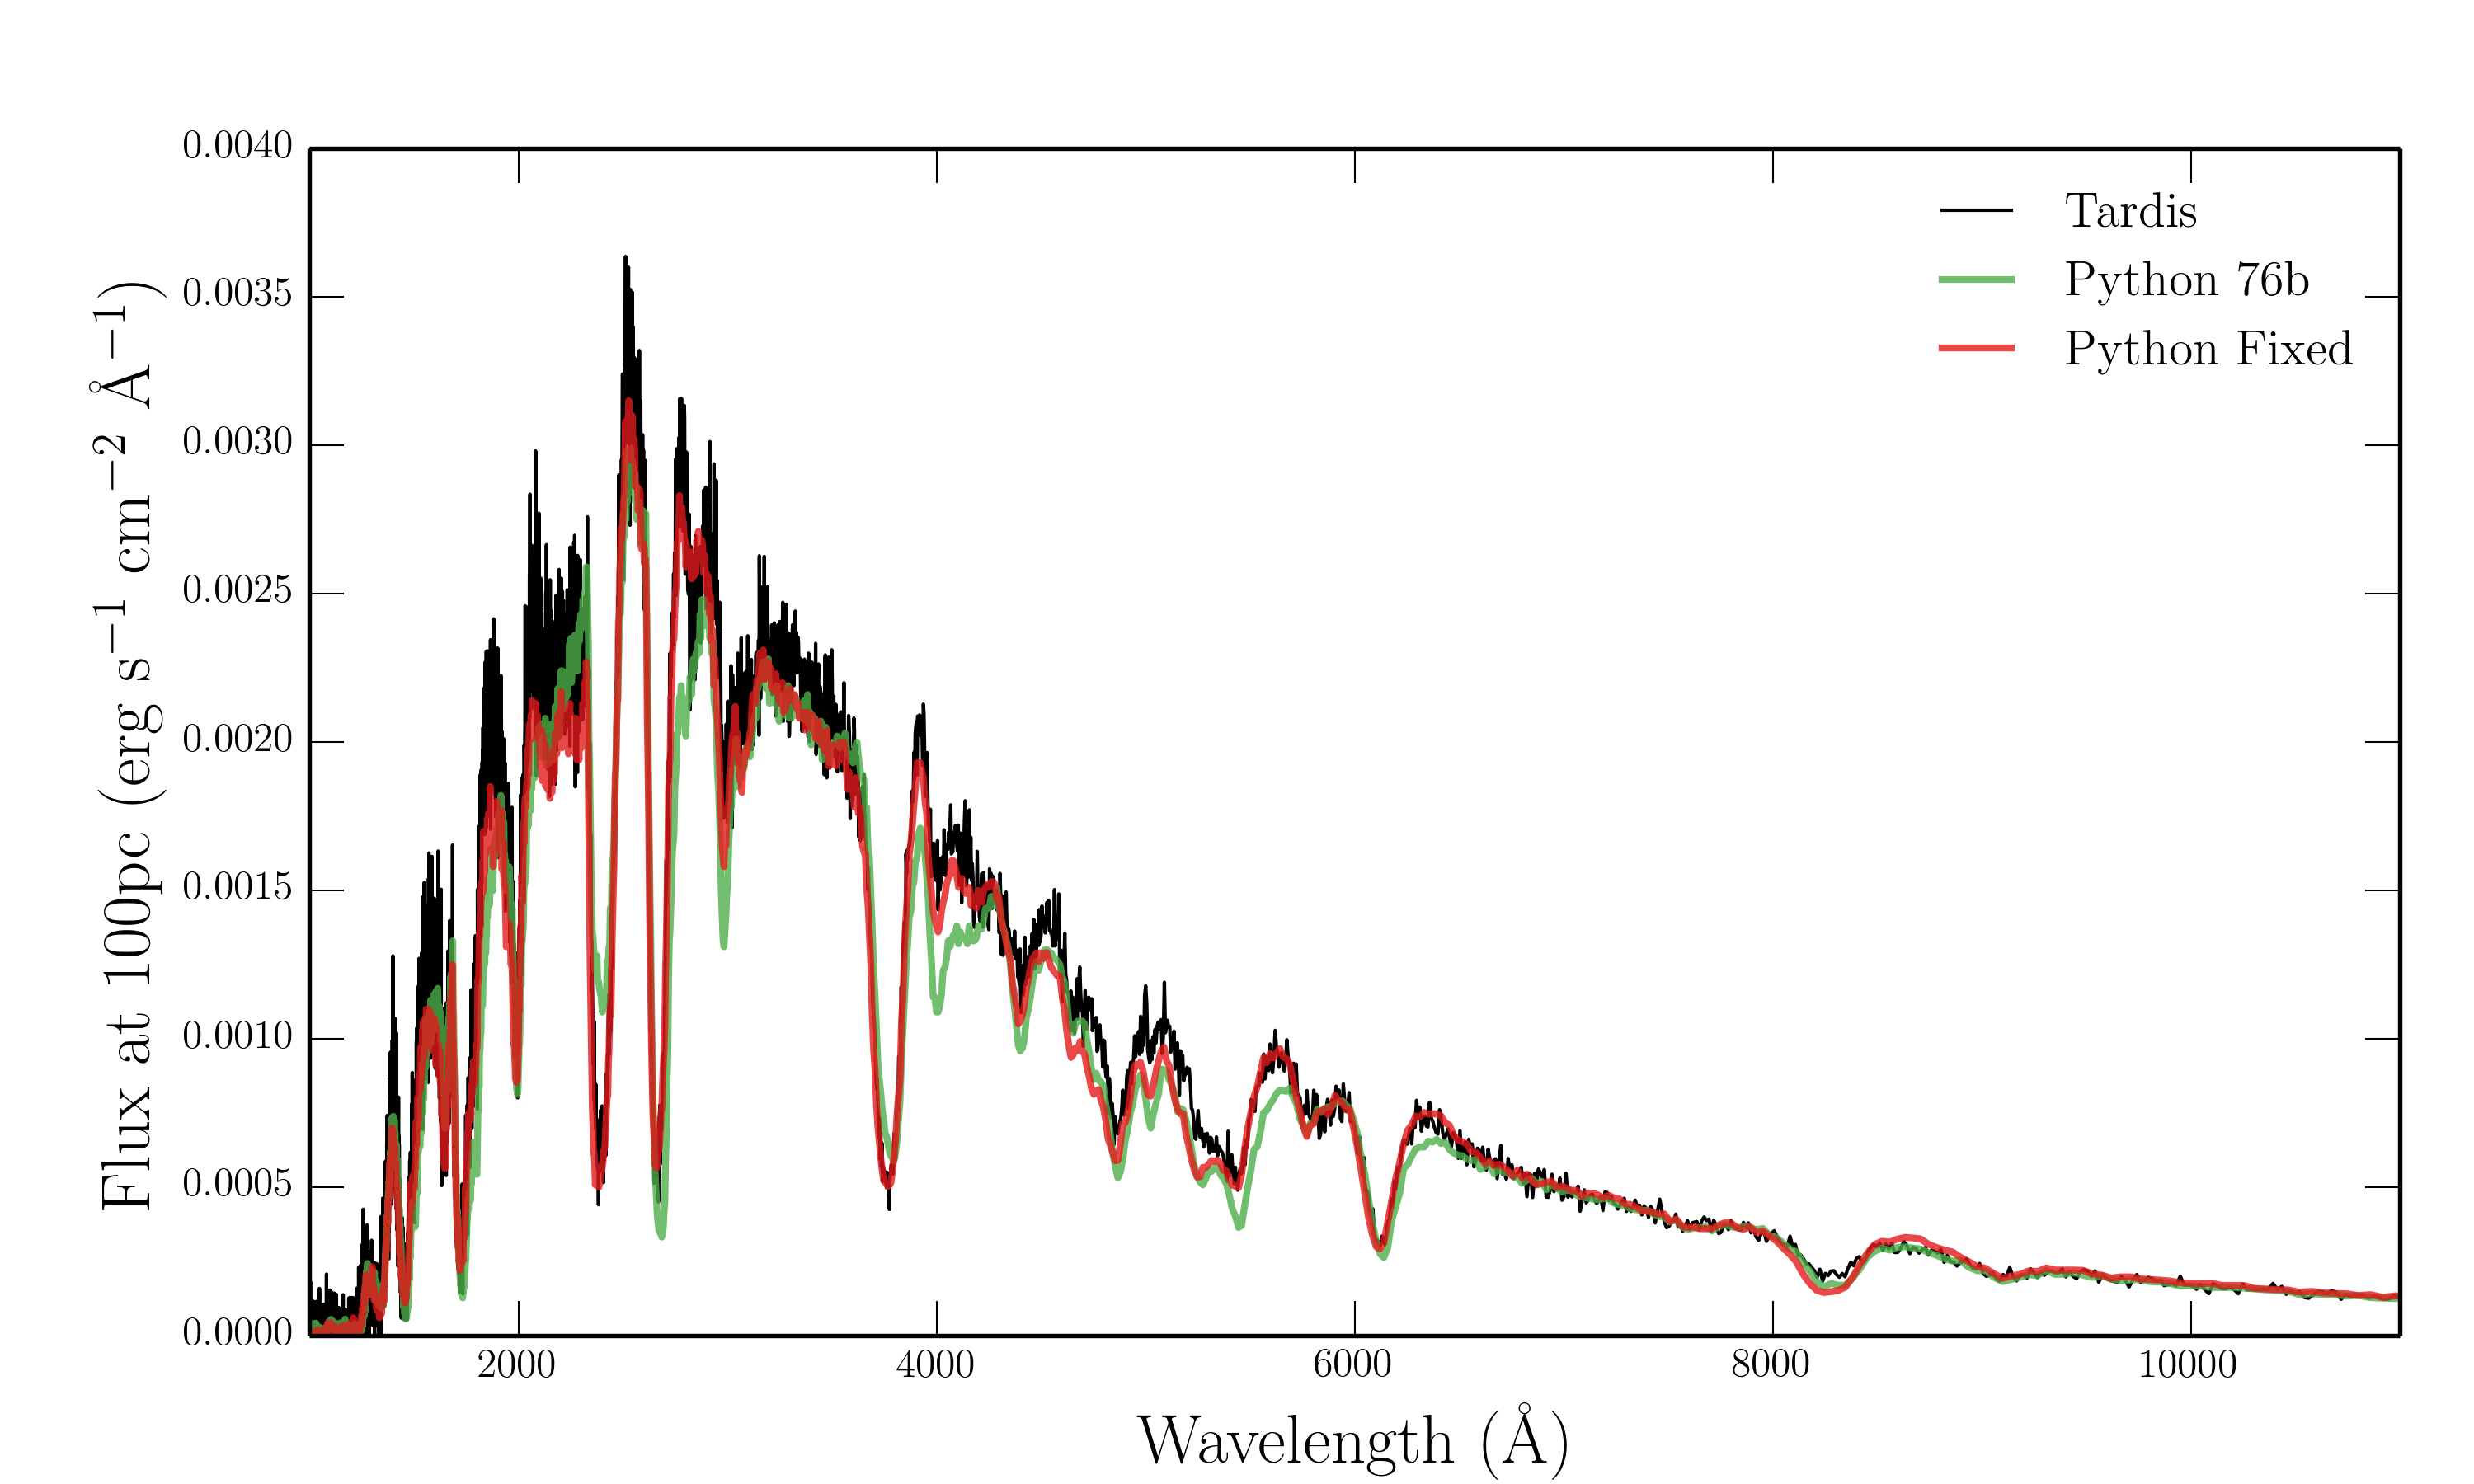
\includegraphics[width=1.0\textwidth]{figures/03-radtrans/tardispython_thesis.png}
\caption[Comparison between \tar\ and \py\ synthetic spectra from 
a simple 1D supernova model.]
{
% {\sl Credit: Kerzendorf \& Sim 2014}.
Comparison between \tar\ and \py\ synthetic spectra from 
a simple 1D supernova model. A bug in Doppler shifting of
photons was discovered around \py\ 76, meaning that the code now gives
even better agreement than presented in Kerzendorf \& Sim 2014.
% $\delta$ is an additional parameter that can be included in the ML93 equation,
% and thus the appropriate comparison here is with the $\delta=1$ case.
}
\label{fig:tardis_spec}
\end{figure}

\subsection{Testing Line Transfer Modes}
\label{sec:line_test}
The simple-atom approach has a few drawbacks. The first is that it cannot
deal well with lines in which the lower level is an excited state, such as the 
Balmer lines. This means that it is important to treat recombination lines using the 
macro-atom approach. The second is that a bound-free continuum activation, 
in normal terms a photoionization, is followed by a radiative deactivation
with the frequency chosen assuming a hydrogenic cross-section. 
This does not well represent reality where recombining
electrons tend to do so to a variety of levels and so there is a gradual
redshifting of the radiation field, and also atoms are in general not hydrogenic. 
This problem has wider implications than
the first, as it could mean that the global ionization and temperature structure of the wind
was affected, if, for example, opacities due to elements such as C, N and O were important
in determining the ionizing radiation field.

To verify that this is a second order effect, 
I have shown a test in Fig.~\ref{fig:line_transfer} in I have tested the indivisible
line transfer mode against weight reduction mode, which does not make this 
approximation. The model shown is the fiducial BAL quasar model from
H13, where modelling the aborption effect on the ionizing radiation field 
properly is important due to the stratified
and self-shielding flow. As long as H and He are treated as macro-atoms, the agreement
between the modes is good and the ionization structure in the flow is very similar.
Many of the differences in the ionization structure in the flow are actually
caused by the improved treatment of the Balmer and Lyman continua.

\begin{figure}
\centering
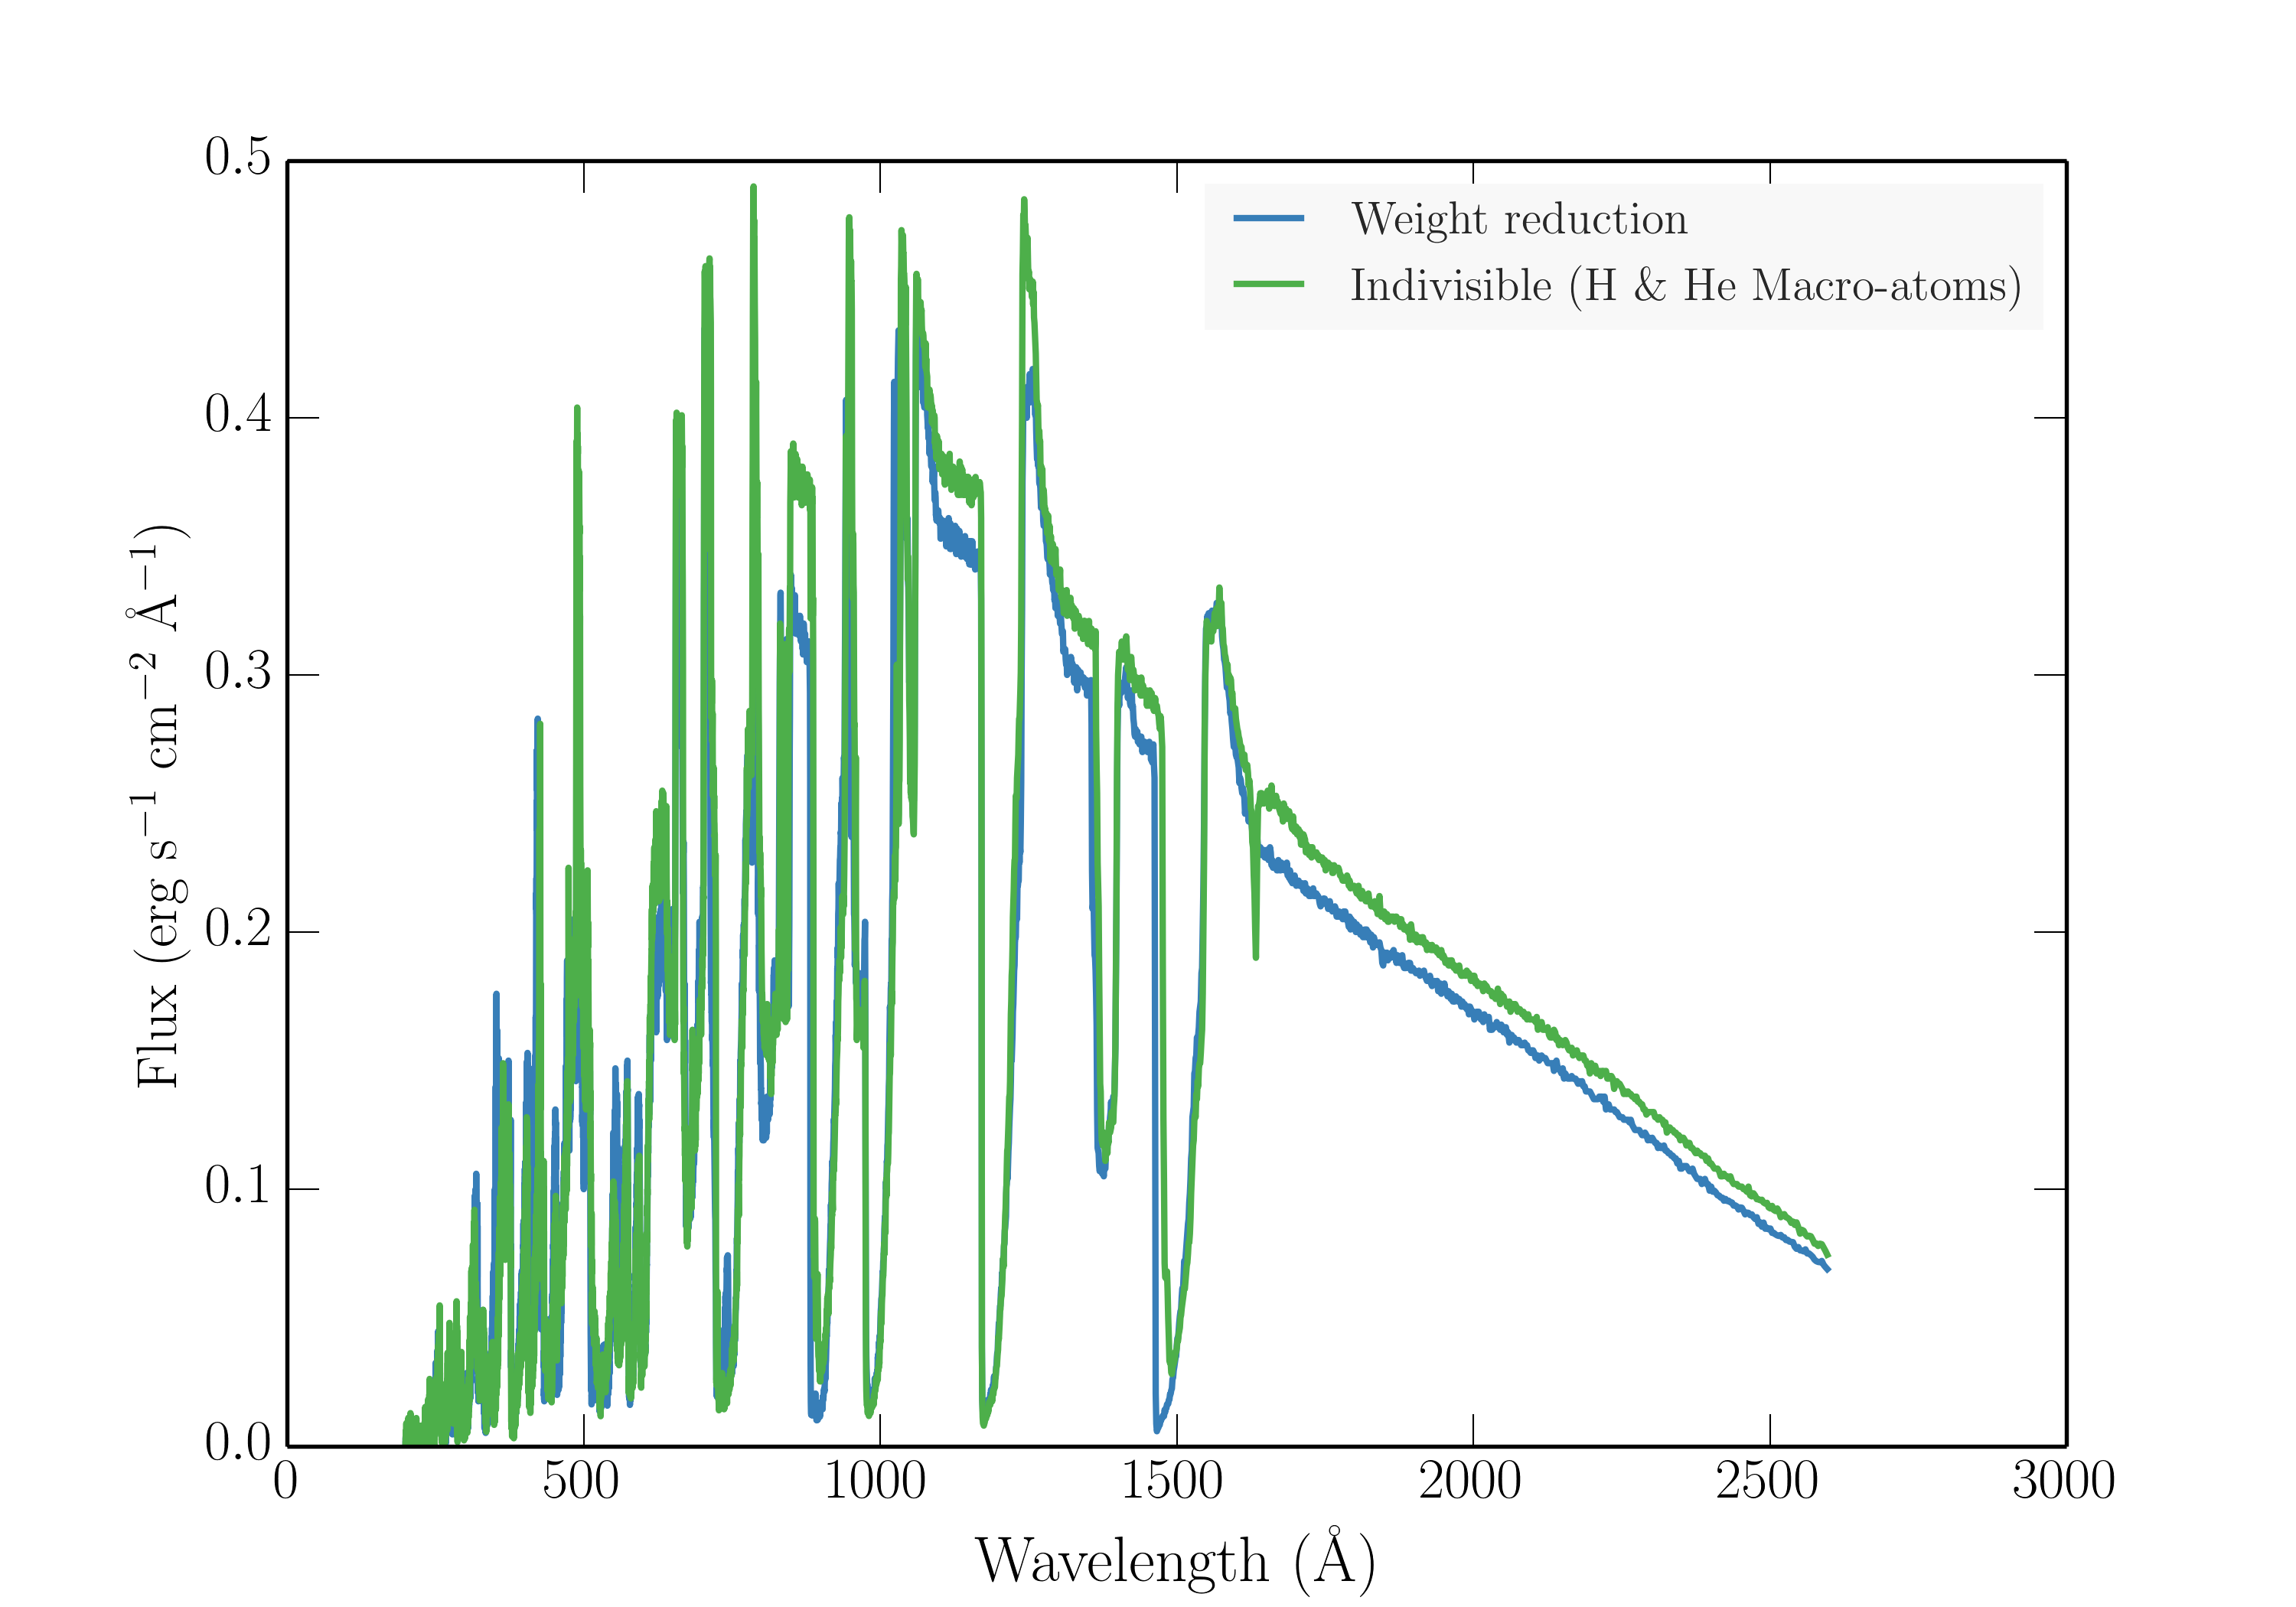
\includegraphics[width=1.0\textwidth]{figures/03-radtrans/line_transfer_comparison.png}
\caption
[A comparison between weight reduction and line transfer mode.]
{
A comparison between weight reduction and line transfer mode. 
The model
} 
\label{fig:line_transfer}
\end{figure}

\section{Code Maintenance and Version Control}
\label{sec:code_maintenance}

As part of the expansion of the team working on \py\, I was responsible
for bringing the code under the auspices of a robust version control system.
Thanks to these efforts, the code is now hosted on GitHub at 
\url{https://github.com/agnwinds/python/}. Our team uses a Pull \& Fork model
for collaborative code development, in which major changes are made in a 
forked repository before the developer submits a `Pull request' to the main 
repository. To test the code, we use a combination of Travis CI build tests 
-- run per commit to the upstream repository -- and our own test suite which is 
run every night on a multi-core server. 

\begin{figure}
\centering
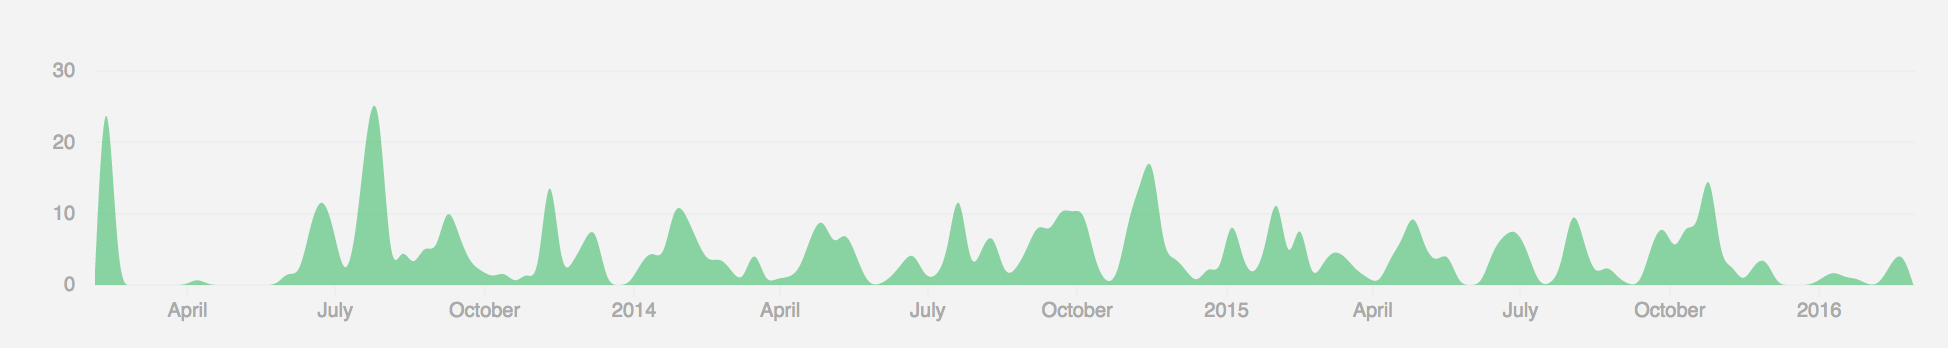
\includegraphics[width=1.0\textwidth]{figures/03-radtrans/github1.png}
\caption
[Github commit history for \py\ from 2013-2016.]
{
Commit history from Feb 3, 2013 to Feb 29, 2016, showing the regular code development
that makes version control such a necessity to a collaborative code project. Produced
using the Github API and plotting capability.
} 
\label{fig:github}
\end{figure}

\subsection{Parallelisation} 
\label{sec:parallel}

Including macro-atoms in a simulation can have a significant impact 
on runtime, especially when simulating dense regions of plasma. 
By way of example, the CV model presented by LK02 takes approximately
118s to run one ionization cycle with $10^6$ photons. One of the macro-atom 
models presented in chapter 4 takes 5651s to complete the same task. 

Fortunately, MCRT codes are intuitively parallelisable, as is the macro-atom
emissivity calculation described above, as operations on cells or photons can
simply be divided up between processors. \py\ is parallelised using an open 
source Message Passing Interface (MPI) implementation known as 
Open MPI \citep{openmpi}. This library provides the core functions needed
in order to share out computing tasks among a series of parallel processors
with distributed memory. The parallelised elements of \py\ include
the photon propagation, updating of wind ionization and temperature structure
and calculation of macro-atom emissivities. As a result, this involves
a reasonable amount of book-keeping in that the radiation field estimators 
must be communicated between threads so as to correctly account for all
the photons that have interacted with a given cell. I have been responsible
for all of the parallelisation implemented that is
specific to the macro-atom routines.

Fig.~\ref{fig:para_times} shows the effect of parallelising a run. Due to the nature of MCRT,
it is possible to achieve significant decrease in overall 
runtime. This improvement was crucial in order to be able to run the simulation
grids used for chapters 4 and 5.


\begin{figure}
\centering
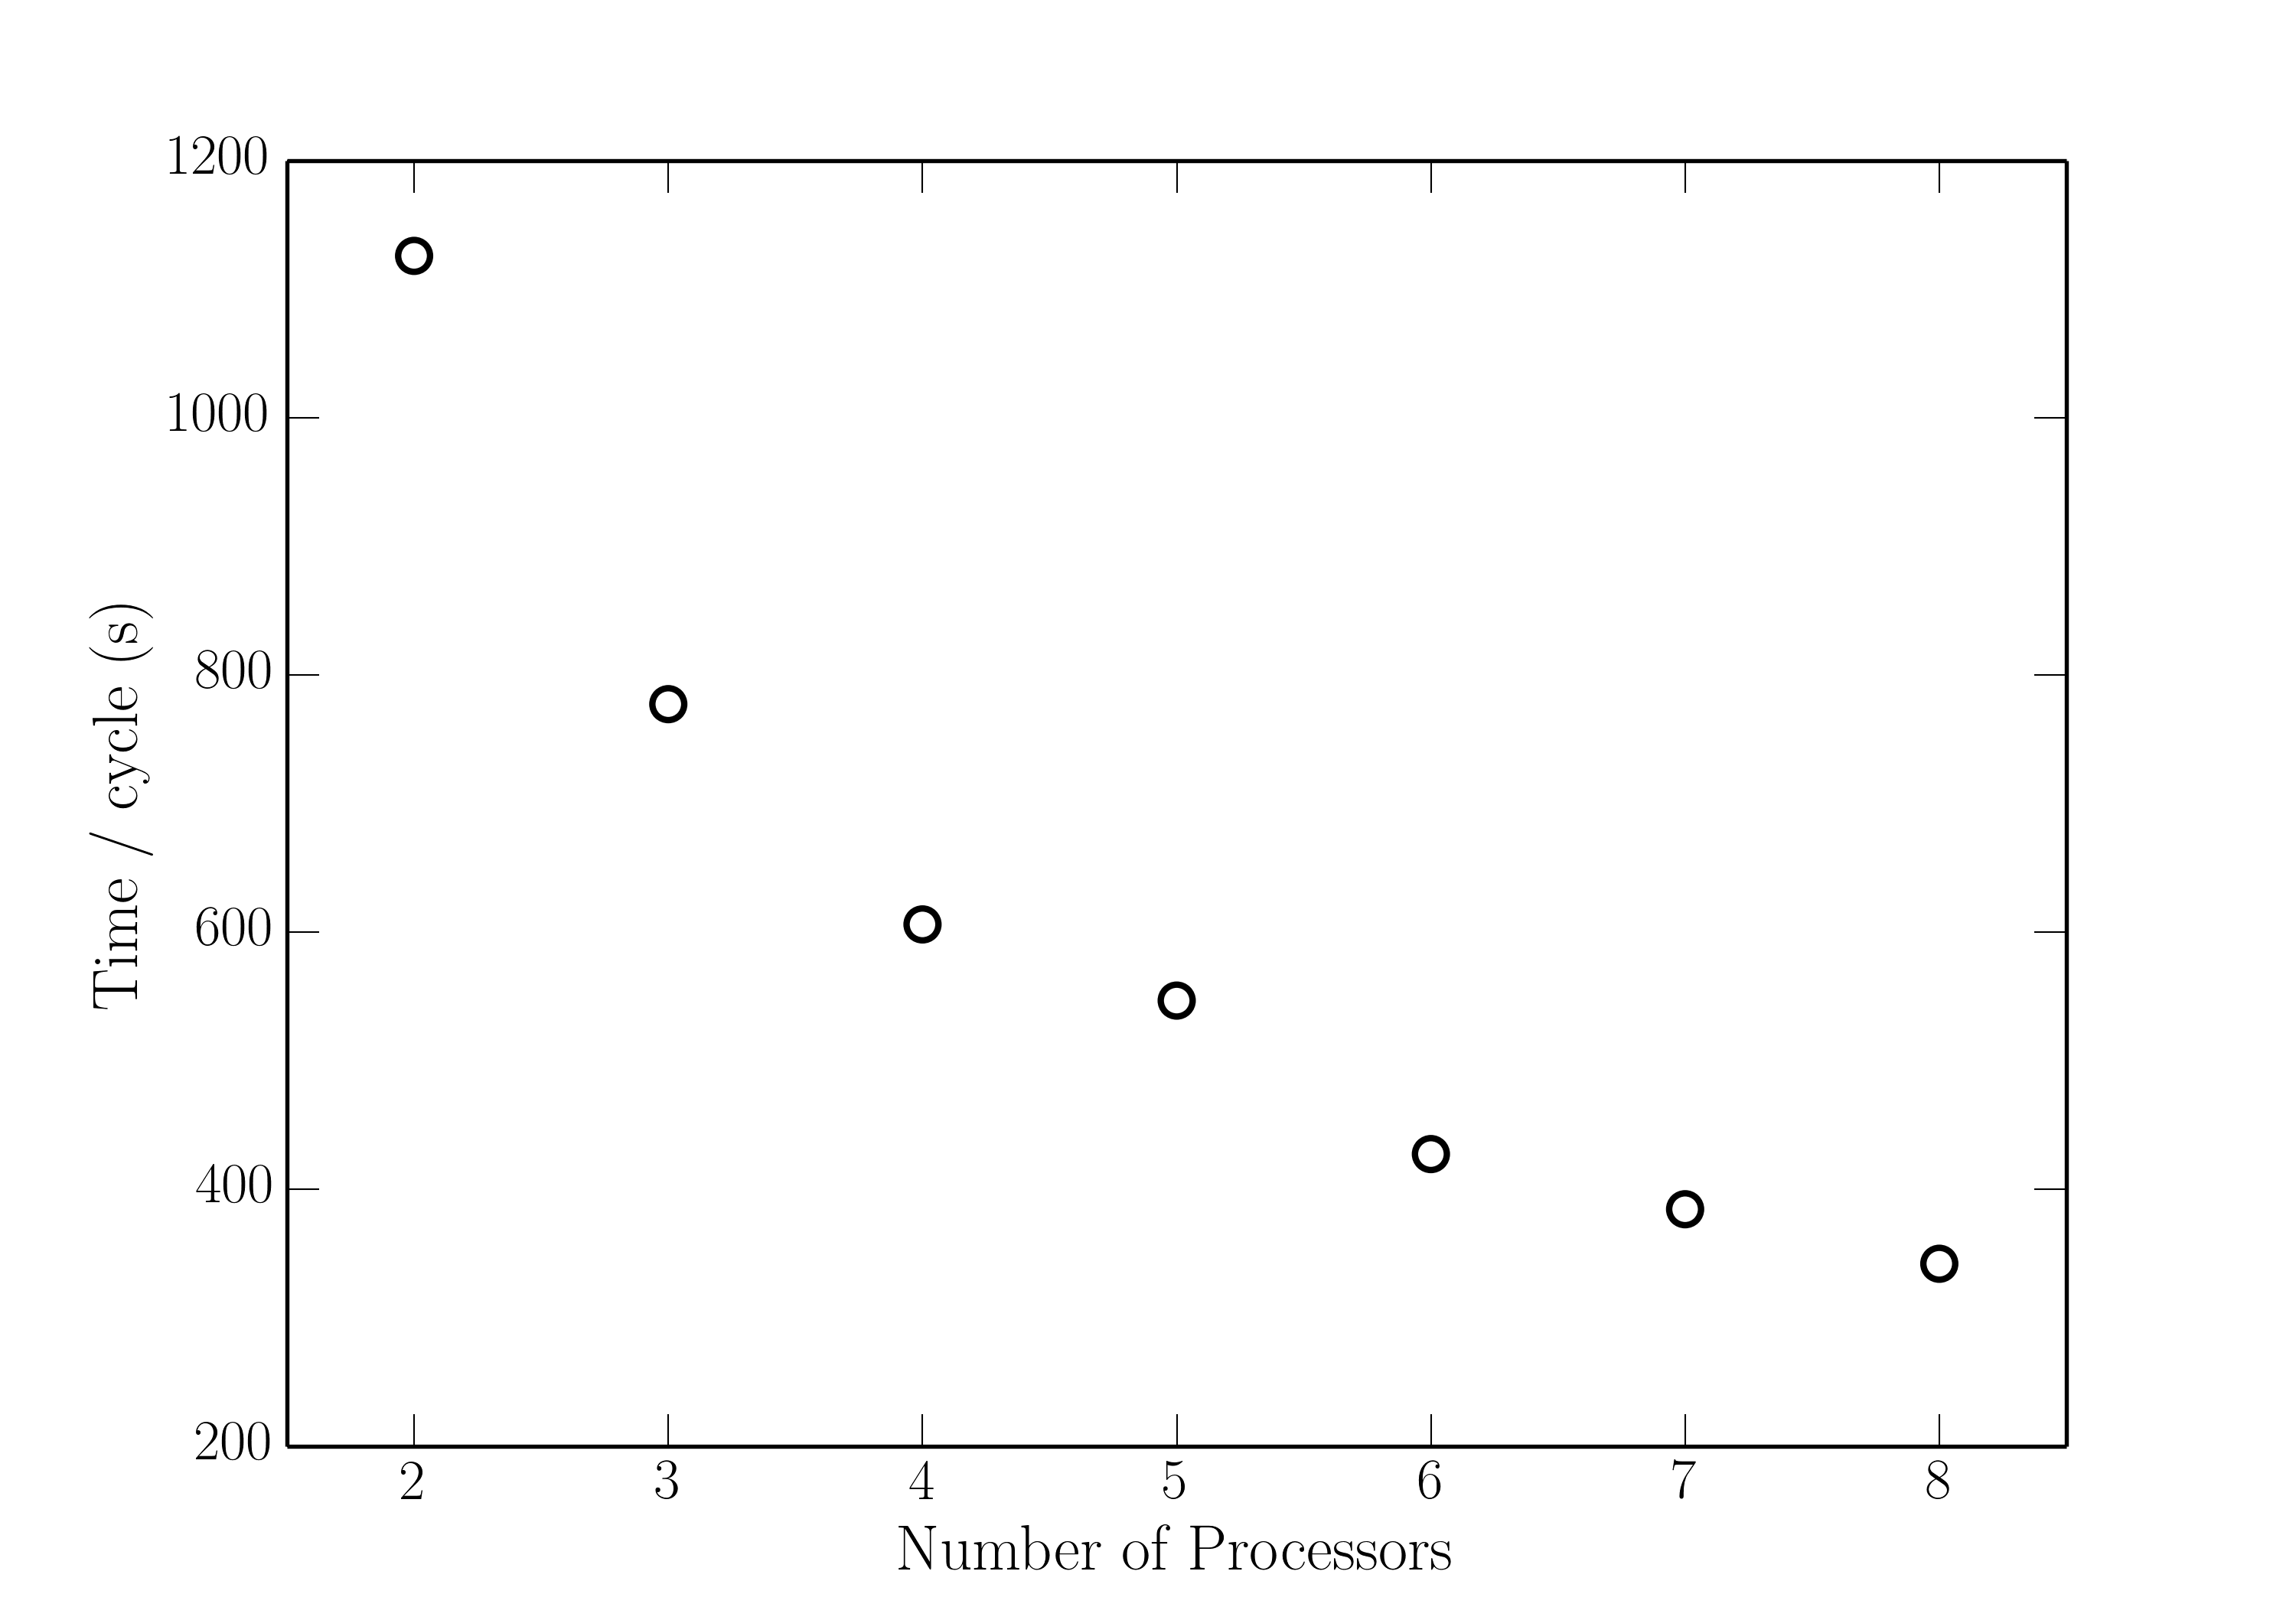
\includegraphics[width=1.0\textwidth]{figures/03-radtrans/para_times.png}
\caption
[Total runtime per cycle for an AGN run as a 
function of the number of processors.]
{
Total runtime per cycle for an AGN run as a 
function of the number of processors.
} 
\label{fig:para_times}
\end{figure}


% \section{My Contribution}

% The code and techniques described represent a large collaborative effort
% by a number of different people. It is therefore important to clearly
% identify my specific contribution to the above work.

% \begin{itemize}
% 	\item Parallelisation of the macro-atom estimators (so they are correctly communicated between threads), and the emissivity calculation described in section~??.
% 	\item Improvement of photoionization cross-sections as described in section~??.
% 	\item Incorporation of Helium macro-atom atomic data.
% 	\item Tabulation of VFKY photoionization cross-sections to avoid on the fly calculations
% 	from the fitting formulae.  
% \end{itemize}







